\documentclass[12pt,a4paper]{report}

% ============================================================
% PRÉAMBULE
% ============================================================
% : Encodage et langue : 
\usepackage[utf8]{inputenc}
\usepackage[T1]{fontenc}
\usepackage{lmodern}
\usepackage[french]{babel}
\usepackage[protrusion=true,expansion=false,spacing=false]{microtype}
\setlength{\emergencystretch}{3em}
\setlength{\hbadness}{10000}

% : Géométrie et mise en page (conforme Instructions : marges 2,5 cm, interligne 1,5) : 
\usepackage[top=2.5cm, bottom=2.5cm, left=2.5cm, right=2.5cm]{geometry}
\usepackage{setspace}
\onehalfspacing
\usepackage{ragged2e}

% : Maths : 
\usepackage{amsmath,amssymb}

% : Couleurs (palette IONIS moderne) : 
\usepackage[dvipsnames,table]{xcolor}
\definecolor{axonbase}{RGB}{30,64,175}      % bleu indigo principal
\definecolor{axonaccent}{RGB}{16,185,129}   % vert accent
\definecolor{axongray}{RGB}{107,114,128}    % gris doux
\definecolor{axonlight}{RGB}{239,246,255}   % bleu très clair
\definecolor{axoncard}{RGB}{248,250,252}    % gris très clair
\definecolor{axonink}{RGB}{31,41,55}        % encre
\definecolor{axonstripe}{RGB}{244,247,252}  % alternance des lignes de tableaux

% : Liens : 
\usepackage[colorlinks=true, linkcolor=axonbase, citecolor=axonaccent, urlcolor=axonbase]{hyperref}
\usepackage{xurl}

% : Images : 
\usepackage{graphicx}
\graphicspath{{image/}{../image/}}

% : Tableaux élégants : 
\usepackage{booktabs}
\usepackage{longtable}
\usepackage{array}
\usepackage{colortbl}
\usepackage{tabularx}
\usepackage{multirow}
\setlength{\tabcolsep}{5pt}

% Colonnes de tableau gérant proprement les retours à la ligne (évite les débordements)
\newcolumntype{L}[1]{>{\RaggedRight\arraybackslash}p{#1}}
\newcolumntype{C}[1]{>{\centering\arraybackslash}p{#1}}

% En-tête de tableau bleu clair (texte en gras)
\newcommand{\tblHeader}[1]{\multicolumn{1}{>{\columncolor[RGB]{219,234,254}}c}{%
    \begingroup\bfseries\color[RGB]{30,41,59}#1\endgroup}}

% : Listes : 
\usepackage{enumitem}
\setlist{itemsep=2pt, parsep=0pt, topsep=4pt}

% : Encadrés modernes (notes, exemples, astuces) : 
\usepackage[most]{tcolorbox}
\newtcolorbox{axonnote}[1][]{%
  colback=axonlight, colframe=axonbase, boxrule=0.6pt,
  arc=3pt, left=6pt, right=6pt, top=5pt, bottom=5pt,
  title={\textbf{\color{axonbase}#1}}, coltitle=axonbase,
  fonttitle=\bfseries, breakable
}
\newtcolorbox{axonexample}[1][]{%
  colback=axoncard, colframe=axonaccent, boxrule=0.6pt,
  arc=3pt, left=6pt, right=6pt, top=5pt, bottom=5pt,
  title={\textbf{\color{axonaccent}#1}}, coltitle=axonaccent,
  fonttitle=\bfseries, breakable
}

% : Code : 
\usepackage{listings}
\lstset{
  basicstyle=\ttfamily\small\color{axonink},
  keywordstyle=\color{axonbase}\bfseries,
  commentstyle=\color{axongray},
  stringstyle=\color{axonaccent},
  breaklines=true,
  frame=single,
  rulecolor=\color{axonlight},
  backgroundcolor=\color{axoncard},
  columns=fullflexible,
  tabsize=2,
  literate=
    {á}{{\'a}}1 {à}{{\`a}}1 {â}{{\^a}}1 {ä}{{\"a}}1
    {é}{{\'e}}1 {è}{{\`e}}1 {ê}{{\^e}}1 {ë}{{\"e}}1
    {í}{{\'i}}1 {ì}{{\`i}}1 {î}{{\^i}}1 {ï}{{\"i}}1
    {ó}{{\'o}}1 {ò}{{\`o}}1 {ô}{{\^o}}1 {ö}{{\"o}}1
    {ú}{{\'u}}1 {ù}{{\`u}}1 {û}{{\^u}}1 {ü}{{\"u}}1
    {ý}{{\'y}}1 {ÿ}{{\"y}}1
    {ç}{{\c c}}1 {ñ}{{\~n}}1
    {É}{{\'E}}1 {È}{{\`E}}1 {Ê}{{\^E}}1 {Ë}{{\"E}}1
    {À}{{\`A}}1 {Â}{{\^A}}1 {Ä}{{\"A}}1
    {Î}{{\^I}}1 {Ï}{{\"I}}1
    {Ô}{{\^O}}1 {Ö}{{\"O}}1
    {Û}{{\^U}}1 {Ü}{{\"U}}1
    {Ç}{{\c C}}1
}

% : Définitions de langages pour listings : 
\lstdefinelanguage{bash}{
  alsoletter={\~/_<>.}, % custom tolerant parsing
  morekeywords={curl,-X,-H,-d,GET,POST,PUT,DELETE,http,https,localhost,Authorization,Bearer,Content-Type},
  sensitive=false,
  morecomment=[l]{\#},
  morestring=[b]",
}
\lstdefinelanguage{json}{
  morekeywords={true,false,null},
  sensitive=true,
}

% : En-têtes et pieds de page : 
\usepackage{fancyhdr}
\pagestyle{fancy}
\setlength{\headheight}{24.6pt}
\addtolength{\topmargin}{-12pt}
\fancyhf{}
\fancyhead[L]{\small\color{axongray}\leftmark}
\fancyhead[R]{\small\color{axongray}\thepage}
\renewcommand{\headrulewidth}{0.4pt}
\renewcommand{\headrule}{\hbox to\headwidth{\color{axonbase}\leaders\hrule height \headrulewidth\hfill}}

% : Style des chapitres et sections : 
\usepackage{titlesec}
\titleformat{\chapter}[display]
  {\normalfont\sffamily\bfseries\color{axonink}}
  {\flushright{\color{axonbase}\fontsize{60}{60}\selectfont\thechapter}\color{axonaccent}\rule[-8pt]{0.2\textwidth}{4pt}\hspace{2pt}\raggedleft}
  {10pt}
  {\fontsize{26}{30}\selectfont}
  [\vspace{2pt}{\color{axonlight}\titlerule[1.2pt]}]
\titlespacing*{\chapter}{0pt}{0pt}{30pt}
\titleformat{\section}
  {\normalfont\sffamily\Large\bfseries\color{axonbase}}
  {\color{axonaccent}\rule{0.5em}{1.2pt}\;\thesection}{0.6em}{}
\titlespacing*{\section}{0pt}{14pt}{6pt}
\titleformat{\subsection}
  {\normalfont\sffamily\large\bfseries\color{axonink}}
  {\thesubsection}{0.7em}{}
\titlespacing*{\subsection}{0pt}{10pt}{4pt}
\titlespacing*{\subsubsection}{0pt}{8pt}{3pt}

% : Légendes : 
\usepackage{caption}
\captionsetup{font=small, labelfont={bf,color=axonbase}, justification=centering, skip=6pt}

% : Prévention des débordements de texte hors de la page : 
\sloppy

% : Metadata : 
\hypersetup{
  pdftitle={Rapport de Stage Pré-MSc 2026 -- Alumni CRM},
  pdfauthor={Rafik Djemadi},
  pdfsubject={Conception et développement d'un Alumni CRM},
  pdfkeywords={alumni, CRM, RGPD, FastAPI, React, PostgreSQL}
}

\begin{document}

% ============================================================
% PAGE DE GARDE (moderne)
% ============================================================
\begin{titlepage}
\thispagestyle{empty}
\begin{tikzpicture}[remember picture,overlay]
  % Bandeau supérieur IONIS (18)
  \fill[axonbase] (current page.north west) rectangle ([yshift=-4.2cm]current page.north east);
  \fill[axonaccent] ([yshift=-4.2cm]current page.north west) rectangle ([yshift=-4.35cm]current page.north east);
  \fill[axonlight] ([yshift=-4.35cm]current page.north west) rectangle ([yshift=-4.5cm]current page.north east);
  % Reliure verticale marine pleine sur le bord droit
  \fill[axonbase] (current page.north east) rectangle ([xshift=-0.9cm]current page.south east);
  \fill[axonaccent] ([xshift=-0.9cm]current page.north east) rectangle ([xshift=-1.05cm]current page.south east);
\end{tikzpicture}

\begin{center}
% En-tête IONIS
{\color{white}\sffamily\bfseries\fontsize{22}{26}\selectfont IONIS Education Group}\\[0.1cm]
{\color{white}\sffamily\large IONIS-STM\quad$\bullet$\quad Programme Pré-MSc}

\vspace{2.4cm}

% 1. Titre centré en haut, bleu et gras (2 lignes)
{\color{axonbase}\sffamily\bfseries\Huge Rapport de Stage}\\[0.25cm]
{\color{axonbase}\sffamily\bfseries\LARGE Pré-MSc 2026}

\vspace{1.4cm}

% 2. Encadré fond bleu clair, texte centré en gras : titre du sujet
\begin{tcolorbox}[
  colback=axonlight, colframe=axonbase,
  width=.84\textwidth, arc=5pt, boxrule=0.8pt, left=12pt, right=12pt, top=10pt, bottom=10pt,
  coltext=axonink
]
\centering\sffamily\Large\bfseries
Conception et développement d'un système de suivi du parcours étudiant et de valorisation du réseau des anciens (Alumni CRM)
\end{tcolorbox}

\vspace{1.8cm}

% 3. Nom de l'auteur en gras, grande taille, centré
{\sffamily\bfseries\Huge Rafik Djemadi}\\[0.25cm]

% 4. Ligne centrée sous le nom
{\sffamily\large Stage de substitution : Pré-MSc 2026}

\vfill

% 5. Bloc d'infos sur deux colonnes avec labels en gras
{\sffamily\large
\begin{tabular}{@{}l@{\hspace{0.5cm}}l@{}}
  \textbf{Auteur :}   & Rafik Djemadi \\
  \textbf{Formation :} & Pré-MSc : IONIS-STM \\[0.5cm]
  \textbf{Tuteur pédagogique :} & Joly Donfack \\
  \textbf{Soutenance :} & 18 septembre 2026 \\
\end{tabular}
}

\vspace{0.9cm}

% 6. Une ligne centrée : période du stage
{\sffamily\large \textbf{Période du stage :} stage de substitution (programme Pré-MSc 2026)}

\vspace{0.5cm}
\end{center}
\end{titlepage}

% ============================================================
% TABLE DES MATIÈRES
% ============================================================
\newpage
\tableofcontents
\newpage

% ============================================================
% RÉSUMÉ (1 page)
% ============================================================
\chapter*{Résumé}
\addcontentsline{toc}{chapter}{Résumé}

\begin{tcolorbox}[
  colback=white, colframe=axonbase, colbacktitle=axonbase,
  coltitle=white, title={Résumé}, fonttitle=\bfseries\sffamily,
  arc=4pt, boxrule=0.8pt, left=14pt, right=14pt, top=10pt, bottom=10pt
]
\sffamily
Ce stage, réalisé au sein d'\hyperlink{abbr-IONIS}{IONIS~(18)}-STM dans le cadre du programme \textbf{Pré-\hyperlink{abbr-MSc}{MSc~(26)} 2026}, porte sur la conception et le développement d'un \textbf{Alumni \hyperlink{abbr-CRM}{CRM~(5)}}~: un système web centralisé destiné au suivi du parcours étudiant et à la valorisation du réseau des anciens diplômés.

\medskip
La problématique identifiée était l'absence d'un outil centralisé permettant à un établissement d'enseignement supérieur de suivre le cycle de vie de ses étudiants (de l'inscription administrative à l'évolution professionnelle post-diplôme) et de disposer d'indicateurs d'insertion fiables pour le pilotage de la formation. Les données d'insertion étaient dispersées, les indicateurs calculés manuellement, le réseau alumni inactif et la conformité \hyperlink{abbr-RGPD}{RGPD~(40)} non formalisée.

\medskip
La démarche a consisté à concevoir et développer une application complète (backend, base de données, frontend et conformité réglementaire), en suivant une approche itérative. Le système repose sur une architecture \textbf{3-tiers} (FastAPI, \hyperlink{abbr-React}{React~(37)}/\hyperlink{abbr-Vite}{Vite~(47)}, \hyperlink{abbr-PostgreSQL}{PostgreSQL~(33)}) avec \textbf{14 tables} de base de données, \textbf{84 endpoints} \hyperlink{abbr-API}{API~(1)}, \textbf{14 routes} frontend et \textbf{8 indicateurs de base} d'insertion professionnelle, complétés d'un indicateur dérivé pour chaque question taguée \hyperlink{abbr-KPI}{KPI~(23)} active.

\medskip
Le projet a abouti à un \textbf{prototype fonctionnel} couvrant l'intégralité du périmètre défini dans le sujet de stage. La conformité \hyperlink{abbr-RGPD}{RGPD~(40)} a été intégrée dès la conception~: consentements traçables, workflow de demandes de suppression et d'anonymisation, journal d'audit et durée de conservation affichée. Un audit de sécurité a permis de corriger des failles d'authentification et de protéger des routes initialement ouvertes. Les livrables documentaires complémentaires (cartographie des données, charte \hyperlink{abbr-RGPD}{RGPD~(40)}, stratégie de mise à jour, analyse des indicateurs d'insertion et guide des processus d'animation du réseau) couvrent les exigences du volet Management du sujet de stage.
\end{tcolorbox}

\begin{tcolorbox}[
  colback=axonlight, colframe=axongray, arc=4pt, boxrule=0.8pt,
  left=12pt, right=12pt, top=8pt, bottom=8pt
]
\noindent\textbf{Mots-clés~:} alumni, \hyperlink{abbr-CRM}{CRM~(5)}, insertion professionnelle, \hyperlink{abbr-RGPD}{RGPD~(40)}, FastAPI, \hyperlink{abbr-React}{React~(37)}, \hyperlink{abbr-PostgreSQL}{PostgreSQL~(33)}, gouvernance des données, indicateurs.
\end{tcolorbox}

\vspace{0.7cm}

\noindent\textbf{Abstract.}

\begin{tcolorbox}[
  colback=white, colframe=axongray, arc=4pt, boxrule=0.8pt,
  left=14pt, right=14pt, top=10pt, bottom=10pt
]
This internship, completed at \hyperlink{abbr-IONIS}{IONIS~(18)}-STM as part of the 2026 Pre-\hyperlink{abbr-MSc}{MSc~(26)} program, focuses on designing and building an \textbf{Alumni \hyperlink{abbr-CRM}{CRM~(5)}}: a centralized web application for tracking student career paths and strengthening the alumni network.

\medskip
The core issue was the lack of a unified tool enabling a higher-education institution to monitor students throughout their entire journey (from initial enrollment to post-graduation professional development) and to produce reliable insertion indicators for program evaluation. Student data was scattered across disconnected channels, insertion rates were computed manually, the alumni network was dormant, and \hyperlink{abbr-GDPR}{GDPR~(14)} compliance had not been formalized.

\medskip
The approach followed an iterative cycle: data modeling, backend development, frontend implementation, security audit, and documentation. The resulting system is built on a 3-tier architecture (FastAPI, \hyperlink{abbr-React}{React~(37)}/\hyperlink{abbr-Vite}{Vite~(47)}, \hyperlink{abbr-PostgreSQL}{PostgreSQL~(33)}) and includes \textbf{14 database tables}, \textbf{84 \hyperlink{abbr-API}{API~(1)} endpoints}, \textbf{14 frontend routes}, and \textbf{8 professional insertion indicators}.

\medskip
The project delivered a functional prototype covering the full scope defined in the internship brief. \hyperlink{abbr-GDPR}{GDPR~(14)} compliance was embedded from the start: traceable consent management, a deletion/anonymization request workflow, an audit log, and visible data retention periods. A security audit led to the correction of authentication flaws and the protection of initially unprotected routes. Supplementary documentation (data mapping, \hyperlink{abbr-GDPR}{GDPR~(14)} charter, update strategy, insertion indicator analysis, and alumni network process guide) fulfills the Management track requirements of the internship specification.
\end{tcolorbox}

\begin{tcolorbox}[
  colback=axonlight, colframe=axongray, arc=4pt, boxrule=0.8pt,
  left=12pt, right=12pt, top=8pt, bottom=8pt
]
\noindent\textbf{Keywords:} alumni, \hyperlink{abbr-CRM}{CRM~(5)}, professional insertion, \hyperlink{abbr-GDPR}{GDPR~(14)}, FastAPI, \hyperlink{abbr-React}{React~(37)}, \hyperlink{abbr-PostgreSQL}{PostgreSQL~(33)}, data governance, indicators.
\end{tcolorbox}


% ============================================================
% PRÉAMBULE : REMERCIEMENTS (1 page)
% ============================================================
\newpage
\chapter*{Préambule : Remerciements}
\addcontentsline{toc}{chapter}{Préambule : Remerciements}

\section*{Remerciements au tuteur pédagogique}

Je tiens à remercier mon tuteur pédagogique, \textbf{M. Joly Donfack}, pour son accompagnement tout au long de ce stage. Sa disponibilité, la pertinence de ses retours et sa capacité à poser les bonnes questions ont orienté les choix d'architecture et les priorités fonctionnelles du projet. Les points de suivi réguliers m'ont permis de conserver une direction claire malgré l'ampleur du périmètre fonctionnel à couvrir.

\section*{Remerciements à l'équipe et au projet}

Ce stage de substitution, proposé directement par \hyperlink{abbr-IONIS}{IONIS~(18)}-STM, m'a offert un cadre de travail encadré et exigeant. L'absence d'une équipe technique dédiée au projet m'a contraint à structurer seul l'ensemble du processus de développement, de la modélisation du \hyperlink{abbr-MCD}{MCD~(24)} à la rédaction des livrables documentaires. Cette expérience a été formatrice sur le plan de l'autonomie et de la prise de décision technique. Je remercie également les interlocuteurs \hyperlink{abbr-IONIS}{IONIS~(18)}-STM impliqués pour les échanges qui ont enrichi la démarche.

\section*{Remerciements à l'école}

Je remercie \hyperlink{abbr-IONIS}{IONIS~(18)}-STM et son équipe pédagogique pour la qualité de la formation dispensée en Pré-\hyperlink{abbr-MSc}{MSc~(26)}, qui m'a doté des fondamentaux techniques nécessaires à la réalisation de ce projet. Les connaissances acquises en développement web, en modélisation de bases de données et en gestion de projets m'ont permis d'aborder ce stage avec les compétences requises.

% ============================================================
% LISTE DES ABRÉVIATIONS ET GLOSSAIRE
% ============================================================
\newpage
\chapter*{Liste des abréviations et glossaire}
\addcontentsline{toc}{chapter}{Liste des abréviations et glossaire}

\begin{longtable}{@{} l l >{\RaggedRight\arraybackslash}p{12.0cm} @{}}
\toprule
\textbf{N°} & \textbf{Abréviation} & \textbf{Signification} \\
\midrule
\endfirsthead
\toprule
\textbf{N°} & \textbf{Abréviation} & \textbf{Signification} \\
\midrule
\endhead
\bottomrule
\endfoot
\hypertarget{abbr-API}{1} & API & Application Programming Interface : interface de programmation permettant la communication entre le frontend et le backend \\
\hypertarget{abbr-CASCADE}{2} & CASCADE & Mécanisme de clé étrangère PostgreSQL assurant la suppression en cascade des enregistrements liés \\
\hypertarget{abbr-CHECK}{3} & CHECK & Contrainte d'intégrité PostgreSQL limitant les valeurs autorisées dans une colonne d'une table \\
\hypertarget{abbr-CNIL}{4} & CNIL & Commission Nationale de l'Informatique et des Libertés : autorité française en charge du contrôle de la protection des données personnelles \\
\hypertarget{abbr-CRM}{5} & CRM & Customer Relationship Management : système de gestion de la relation client (ici~: Alumni CRM, appliqué au réseau des anciens) \\
\hypertarget{abbr-CRUD}{6} & CRUD & Create, Read, Update, Delete : les quatre opérations de base sur les données \\
\hypertarget{abbr-CSS}{7} & CSS & Cascading Style Sheets : langage de mise en forme utilisé pour styliser les pages web \\
\hypertarget{abbr-CSV}{8} & CSV & Comma-Separated Values : format de fichier tabulaire employé pour l'import/export de données \\
\hypertarget{abbr-CTI}{9} & CTI & Commission des Titres d'Ingénieur : organisme d'accréditation des formations d'ingénieurs en France \\
\hypertarget{abbr-DELETE}{10} & DELETE & Méthode HTTP de suppression d'une ressource (utilisée sur les endpoints de l'API) \\
\hypertarget{abbr-DOCX}{11} & DOCX & Format de document Microsoft Word (.docx), supporté pour l'import de données \\
\hypertarget{abbr-DPO}{12} & DPO & Data Protection Officer : Délégué à la Protection des Données, contact réglementaire RGPD \\
\hypertarget{abbr-E2E}{13} & E2E & End-to-End : type de test couvrant l'ensemble du flux applicatif \\
\hypertarget{abbr-GDPR}{14} & GDPR & General Data Protection Regulation : version anglaise du RGPD \\
\hypertarget{abbr-GET}{15} & GET & Méthode HTTP de lecture d'une ressource (récupération de données) \\
\hypertarget{abbr-HCERES}{16} & HCERES & Haute Autorité pour l'Évaluation de la Recherche et l'Enseignement Supérieur : organisme d'évaluation des formations \\
\hypertarget{abbr-HTML}{17} & HTML & HyperText Markup Language : langage de balisage structurant le contenu des pages web \\
\hypertarget{abbr-IONIS}{18} & IONIS & Groupe IONIS Education : groupe d'enseignement supérieur privé \\
\hypertarget{abbr-IDOR}{19} & IDOR & Insecure Direct Object Reference : faille d'accès permettant de manipuler une ressource via un identifiant \\
\hypertarget{abbr-JSON}{20} & JSON & JavaScript Object Notation : format d'échange de données structurées, utilisé ici pour les réponses API et les réponses de questionnaire \\
\hypertarget{abbr-JSONB}{21} & JSONB & Type de colonne PostgreSQL stockant du JSON de façon binaire optimisée, avec indexation \\
\hypertarget{abbr-JWT}{22} & JWT & JSON Web Token : standard de jeton d'authentification utilisé pour les sessions utilisateur \\
\hypertarget{abbr-KPI}{23} & KPI & Key Performance Indicator : Indicateur Clé de Performance utilisé dans le tableau de bord administrateur \\
\hypertarget{abbr-MCD}{24} & MCD & Modèle Conceptuel de Données : représentation abstraite des entités et relations du système \\
\hypertarget{abbr-MLD}{25} & MLD & Modèle Logique de Données : traduction du MCD en schéma de tables relationnelles \\
\hypertarget{abbr-MSc}{26} & MSc & Master of Science : grade de master délivré par les programmes MSc et Pré-MSc de l'IONIS-STM \\
\hypertarget{abbr-NM}{27} & N:M & Relation many-to-many (cardinalité plusieurs-à-plusieurs), via une table de jonction \\
\hypertarget{abbr-OTP}{28} & OTP & One-Time Password : mot de passe à usage unique, ici code à 6 chiffres envoyé par email \\
\hypertarget{abbr-PATCH}{29} & PATCH & Méthode HTTP de modification partielle d'une ressource \\
\hypertarget{abbr-PDF}{30} & PDF & Portable Document Format : format de document utilisé pour l'export des fiches et rapports \\
\hypertarget{abbr-pg8000}{31} & pg8000 & Pilote PostgreSQL pur Python, utilisé pour la connexion à la base de données \\
\hypertarget{abbr-POST}{32} & POST & Méthode HTTP de création d'une ressource (envoi de données au serveur) \\
\hypertarget{abbr-PostgreSQL}{33} & PostgreSQL & Système de gestion de base de données relationnelle open source \\
\hypertarget{abbr-PUT}{34} & PUT & Méthode HTTP de remplacement complet d'une ressource \\
\hypertarget{abbr-PWA}{35} & PWA & Progressive Web App : application web offrant une expérience proche d'une application native \\
\hypertarget{abbr-Pydantic}{36} & Pydantic & Bibliothèque Python de validation de données basée sur les annotations de type \\
\hypertarget{abbr-React}{37} & React & Bibliothèque JavaScript pour la construction d'interfaces utilisateur \\
\hypertarget{abbr-README}{38} & README & Fichier de documentation d'un dépôt logiciel décrivant l'installation et l'utilisation du projet \\
\hypertarget{abbr-REST}{39} & REST & Representational State Transfer : style d'architecture pour les API web \\
\hypertarget{abbr-RGPD}{40} & RGPD & Règlement Général sur la Protection des Données (Règlement UE 2016/679) : cadre réglementaire européen \\
\hypertarget{abbr-SPA}{41} & SPA & Single Page Application : application web mono-page (architecture React) \\
\hypertarget{abbr-SQL}{42} & SQL & Structured Query Language : langage de requête des bases de données relationnelles (PostgreSQL) \\
\hypertarget{abbr-SVG}{43} & SVG & Scalable Vector Graphics : format d'image vectorielle utilisé pour les graphiques du dashboard \\
\hypertarget{abbr-Swagger}{44} & Swagger & Interface de documentation et d'essai des API, auto-générée par FastAPI \\
\hypertarget{abbr-TOCTOU}{45} & TOCTOU & Time-of-check to time-of-use : type de course (race condition) sur la vérification d'accès \\
\hypertarget{abbr-UE}{46} & UE & Union Européenne : espace juridique au sein duquel s'applique le règlement RGPD \\
\hypertarget{abbr-Vite}{47} & Vite & Outil de build et serveur de développement frontend rapide \\
\hypertarget{abbr-XLSX}{48} & XLSX & Format de classeur Microsoft Excel (.xlsx), supporté pour l'import/export des données alumni \\
\end{longtable}

% ============================================================
% LISTE DES FIGURES ET TABLEAUX
% ============================================================
\newpage
\listoffigures
\addcontentsline{toc}{chapter}{Liste des figures}
\newpage
\listoftables
\addcontentsline{toc}{chapter}{Liste des tableaux}

% ============================================================
% CHAPITRE 1 : CONTEXTE
% ============================================================
% ============================================================
% CHAPITRE 1 : CONTEXTE
% ============================================================
\chapter{Contexte de la structure d'accueil}

\section{Présentation d'IONIS-STM}

\hyperlink{abbr-IONIS}{IONIS~(18)}-STM est une école du groupe \hyperlink{abbr-IONIS}{IONIS~(18)} Education Group, acteur privé de l'enseignement supérieur en France. Le groupe regroupe plusieurs écoles d'ingénieurs et de management (EPITECH, ESGI, ESM, ISA, IIM, ISEN, ICS, entre autres), couvrant les domaines du numérique, de l'ingénierie et du management.

\hyperlink{abbr-IONIS}{IONIS~(18)}-STM dispense des programmes de niveau Pré-\hyperlink{abbr-MSc}{MSc~(26)}, MSc1 et MSc2, ciblant des étudiants en reconversion ou en poursuite d'études après un diplôme initial. Les formations sont organisées en filières spécialisées et débouchent sur des métiers du développement, de la cybersécurité, de la data, du management et du marketing digital.

L'établissement forme chaque année plusieurs centaines de diplômés. Suivre l'insertion professionnelle de ces anciens élèves est un enjeu stratégique pour piloter la formation, respecter les exigences des organismes de tutelle (\hyperlink{abbr-CTI}{CTI~(9)}, \hyperlink{abbr-HCERES}{HCERES~(16)}) et animer le réseau alumni.

\section{Secteur d'activité et acteurs clés}

Le secteur de l'enseignement supérieur privé en France se caractérise par une concurrence croissante entre établissements pour attirer les candidats, garantir l'employabilité des diplômés et maintenir des relations durables avec les entreprises partenaires. Les acteurs clés dans ce contexte sont~:

\begin{itemize}
  \item \textbf{Les étudiants et alumni}~: bénéficiaires des formations, dont la trajectoire professionnelle est le principal indicateur de qualité.
  \item \textbf{Le service des relations entreprises}~: responsable du placement, des partenariats et du suivi de l'insertion.
  \item \textbf{La direction pédagogique}~: pilote l'offre de formation au regard des besoins du marché.
  \item \textbf{Les organismes de certification} (\hyperlink{abbr-CTI}{CTI~(9)}, \hyperlink{abbr-HCERES}{HCERES~(16)})~: exigent des rapports d'insertion réguliers comme condition d'accréditation.
\end{itemize}

\section{Context économique et positionnement}

Le secteur privé de l'enseignement supérieur est porté par la demande croissante en compétences numériques. Le positionnement du groupe \hyperlink{abbr-IONIS}{IONIS~(18)} repose sur un portefeuille d'écoles spécialisées, chacune adressant un domaine (développement, informatique de gestion, marketing digital, agronomie, etc.) tout en partageant une même exigence de placement professionnel et de suivi des diplômés.

Cette organisation en écosystème multi-écoles crée un enjeu commun~: disposer d'un dispositif de suivi alumni scalable, capable de fonctionner à l'échelle de plusieurs centaines de diplômés par promotion sur l'ensemble du groupe.

\section{Problématique spécifique du projet}

L'absence d'un outil centralisé de suivi alumni posait plusieurs problèmes concrets au sein d'\hyperlink{abbr-IONIS}{IONIS~(18)}-STM~:

\begin{enumerate}
  \item \textbf{Données dispersées}~: les informations d'insertion étaient collectées ponctuellement (par email, formulaire papier, appels téléphoniques) sans stockage structuré ni traçabilité.
  \item \textbf{Indicateurs non fiables}~: le calcul des taux d'insertion (à 6 mois, à 12 mois) nécessitait des croisements manuels fastidieux, propices aux erreurs.
  \item \textbf{Réseau inanimé}~: aucun canal structuré ne permettait aux anciens diplômés de maintenir leur profil à jour ni de rester en contact avec l'école.
  \item \textbf{Conformité \hyperlink{abbr-RGPD}{RGPD~(40)} non formalisée}~: la collecte et le traitement des données personnelles des alumni n'obéissaient à aucun workflow traçable.
\end{enumerate}

La problématique du stage était donc de concevoir et développer un système capable de répondre simultanément à ces quatre problèmes, tout en étant conforme aux exigences réglementaires et en fournissant des indicateurs exploitables pour le pilotage.

\section{Enjeux du suivi alumni dans le contexte IONIS}

Le suivi de l'insertion professionnelle des anciens élèves constitue un enjeu à plusieurs niveaux~:

\textbf{Enjeu réglementaire.} Les organismes de tutelle et de certification (la \hyperlink{abbr-CTI}{CTI~(9)} pour les formations d'ingénieurs, le \hyperlink{abbr-HCERES}{HCERES~(16)} pour l'enseignement supérieur) exigent des établissements la communication de rapports d'insertion professionnelle réguliers. Ces rapports contiennent des indicateurs standardisés~: taux d'emploi à 6 mois et à 12 mois après la diplomation, adéquation formation-emploi, répartition par secteur d'activité et par type de contrat. L'absence de données fiables et centralisées rend la production de ces rapports fastidieuse et sujette à erreurs.

\textbf{Enjeu pédagogique.} Le taux d'insertion et la nature des postes occupés par les diplômés constituent des indicateurs de pertinence de l'offre de formation. Si les diplômés d'une filière se dirigent majoritairement vers des secteurs éloignés de la formation reçue, cela signale un décalage entre le programme et les besoins du marché. Le suivi alumni permet d'alimenter cette boucle de rétroaction entre la formation et l'emploi.

\textbf{Enjeu managérial.} Le service des relations entreprises d'un établissement comme \hyperlink{abbr-IONIS}{IONIS~(18)}-STM a besoin de données structurées pour piloter les partenariats avec les entreprises, identifier les secteurs recrutant le plus de diplômés et préparer les événements de networking. Un réseau alumni vivant constitue aussi un levier de fidélisation et de recommandation auprès de futurs candidats.

\textbf{Enjeu technique.} La collecte et le traitement des données personnelles des alumni sont soumis au \hyperlink{abbr-RGPD}{RGPD~(40)}. La conformité réglementaire impose des contraintes fortes sur le consentement, la durée de conservation, le droit d'accès et le droit à l'effacement. Un outil centralisé doit intégrer ces exigences dès la conception.

\section{Positionnement du projet dans la stratégie de l'établissement}

Le projet Alumni \hyperlink{abbr-CRM}{CRM~(5)} s'inscrit dans une démarche de professionnalisation du suivi des anciens élèves au sein d'\hyperlink{abbr-IONIS}{IONIS~(18)}-STM. Il vise à remplacer les processus manuels de collecte de données (emails ponctuels, formulaires papier, appels téléphoniques) par un système structuré et traçable, capable de produire automatiquement les indicateurs requis par les autorités de tutelle.

Le système devait répondre à quatre objectifs fonctionnels définis dans le sujet de stage~:

\begin{itemize}
  \item Créer une solution centralisée permettant de suivre le cycle de vie de l'étudiant, de son inscription administrative jusqu'à son évolution professionnelle post-diplôme.
  \item Fournir des indicateurs d'insertion professionnelle exploitables par le service des relations entreprises.
  \item Assurer la conformité \hyperlink{abbr-RGPD}{RGPD~(40)} de toutes les opérations de collecte et de traitement des données personnelles.
  \item Produire un guide des processus d'animation du réseau alumni.
\end{itemize}

% ============================================================
% CHAPITRE 2 : PRÉSENTATION DU STAGE
% ============================================================
\chapter{Présentation du stage et déroulement des missions}

\section{Contexte précis et objectifs du stage}

Ce stage est un \textbf{stage de substitution}, proposé directement par \hyperlink{abbr-IONIS}{IONIS~(18)}-STM aux étudiants du programme Pré-\hyperlink{abbr-MSc}{MSc~(26)} n'ayant pas trouvé de placement en entreprise. Il s'agit d'un cas de figure explicitement prévu par le programme. La structure d'accueil est \hyperlink{abbr-IONIS}{IONIS~(18)}-STM elle-même, et l'encadrement est assuré par un tuteur pédagogique interne.

Le sujet officiel du stage est~: \textit{\og{}Conception et développement d'un système de suivi du parcours étudiant et de valorisation du réseau des anciens (Alumni \hyperlink{abbr-CRM}{CRM~(5)})\fg{}}.

L'objectif général définissait la création d'une solution centralisée permettant de suivre le \og{}cycle de vie\fg{} de l'étudiant, de son inscription administrative jusqu'à son évolution professionnelle post-diplôme, afin de faciliter le pilotage de l'insertion et l'animation du réseau. Le projet couvrait deux volets complémentaires~: un volet \textbf{Management} (gouvernance des données, conformité \hyperlink{abbr-RGPD}{RGPD~(40)}, indicateurs d'insertion) et un volet \textbf{Informatique} (modélisation de la base, développement de l'application, automatisation).

Les objectifs fonctionnels du projet, définis dans le sujet officiel, étaient~:

\begin{itemize}
  \item Créer une solution centralisée permettant de suivre le cycle de vie de l'étudiant, de son inscription administrative jusqu'à son évolution professionnelle post-diplôme.
  \item Fournir des indicateurs d'insertion professionnelle exploitables par le service des relations entreprises.
  \item Assurer la conformité \hyperlink{abbr-RGPD}{RGPD~(40)} de toutes les opérations de collecte et de traitement des données personnelles.
  \item Produire un guide des processus d'animation du réseau alumni.
\end{itemize}

Les livrables attendus étaient~: le rapport de stage, le schéma conceptuel \hyperlink{abbr-MCD}{MCD~(24)}/\hyperlink{abbr-MLD}{MLD~(25)}, un prototype fonctionnel, et le guide des processus d'animation du réseau.

\section{Missions confiées et responsabilités}

Le stage s'est articulé autour de \textbf{cinq domaines de mission}~:

\subsection{Mission 1 : Modélisation et conception de la base de données}

J'ai conçu un modèle de données relationnel couvrant cinq domaines fonctionnels~: données étudiantes, parcours professionnel, conformité \hyperlink{abbr-RGPD}{RGPD~(40)}, questionnaires et infrastructure technique. Le résultat est une base \hyperlink{abbr-PostgreSQL}{PostgreSQL~(33)} de \textbf{14 tables} organisées en 5 groupes~:

\begin{itemize}
  \item \textit{Données étudiantes}~: ETUDIANT, PROMOTION
  \item \textit{Parcours professionnel}~: ENTREPRISE, EXPERIENCE\_PRO, CERTIFICATION, OBTIENT (association \hyperlink{abbr-NM}{N:M~(27)})
  \item \textit{\hyperlink{abbr-RGPD}{RGPD~(40)}}~: CONSENTEMENT\_RGPD, DEMANDE\_RGPD, AUDIT\_LOG
  \item \textit{Questionnaires}~: QUESTIONNAIRE, QUESTION, REPONSE\_QUESTIONNAIRE
  \item \textit{Infrastructure}~: otp\_codes, schema\_migrations
\end{itemize}

Le passage du \hyperlink{abbr-MCD}{MCD~(24)} au \hyperlink{abbr-MLD}{MLD~(25)} a respecté les règles de transformation standard (entité forte $\rightarrow$ table, association \hyperlink{abbr-NM}{N:M~(27)} $\rightarrow$ table de jonction). J'ai versionné 17 migrations \hyperlink{abbr-SQL}{SQL~(42)} (16 à la date de l'audit de conformité, plus la migration corrective 016 du 10/09/2026), appliquées via un script maison (\texttt{run\_migrations.py}) qui ne rejoue que les migrations non encore exécutées.

\subsection{Mission 2 : Développement du backend API}

J'ai développé une \hyperlink{abbr-API}{API~(1)} \hyperlink{abbr-REST}{REST~(39)} complète avec FastAPI (Python). L'\hyperlink{abbr-API}{API~(1)} comprend \textbf{16 routeurs} et \textbf{84 endpoints} couvrant~:

\begin{itemize}
  \item Authentification (\hyperlink{abbr-OTP}{OTP~(28)} email + code à 6 chiffres, clé d'accès \hyperlink{abbr-API}{API~(1)} admin, sessions \hyperlink{abbr-JWT}{JWT~(22)})
  \item Gestion des promotions et des étudiants/alumni (\hyperlink{abbr-CRUD}{CRUD~(6)} complet)
  \item Entreprises et expériences professionnelles (\hyperlink{abbr-CRUD}{CRUD~(6)} avec création automatique de l'entreprise si inexistante)
  \item Certifications (catalogue + association \hyperlink{abbr-NM}{N:M~(27)})
  \item \hyperlink{abbr-RGPD}{RGPD~(40)} (consentement, demandes de suppression/anonymisation, journal d'audit)
  \item Questionnaires (\hyperlink{abbr-CRUD}{CRUD~(6)} admin + soumission alumni avec validation des clés)
  \item Dashboard administrateur (indicateurs, statistiques, filtrage, évolution temporelle)
  \item Import/export (template Excel, import alumni \hyperlink{abbr-CSV}{CSV~(8)}/Excel avec détection automatique du séparateur, export complet)
  \item Nettoyage (détection d'orphelins, fusion de doublons, archivage, purge différée)
\end{itemize}

\subsection{Mission 3 : Développement du frontend React}

J'ai développé une interface utilisateur complète avec \hyperlink{abbr-React}{React~(37)} + \hyperlink{abbr-Vite}{Vite~(47)}, structurée en deux espaces~:

\begin{itemize}
  \item \textit{Espace administrateur}~: tableau de bord avec \hyperlink{abbr-KPI}{KPI~(23)} et graphiques, annuaire filtrable, gestion des promotions, import/export Excel, gestion des questionnaires, traitement des demandes \hyperlink{abbr-RGPD}{RGPD~(40)}.
  \item \textit{Espace alumni}~: inscription multi-étapes, vérification \hyperlink{abbr-OTP}{OTP~(28)}, édition de profil, parcours professionnel (expériences et certifications en ajout/suppression, la modification d'une expérience existante étant désormais supportée via \texttt{\hyperlink{abbr-PUT}{PUT~(34)} /experiences/\{id\_experience\}} en une seule transaction atomique), consentement \hyperlink{abbr-RGPD}{RGPD~(40)}, questionnaire annuel.
\end{itemize}

Le frontend comprend \textbf{14 routes principales} et des composants partagés (thème clair/sombre, indicateurs, protection de routes par rôle). La validation des composants repose sur des tests manuels et la vérification du build de production (\texttt{vite build}) ainsi que du lint (\texttt{oxlint})~; aucune suite de tests automatisés n'est conservée dans le dépôt à l'issue du stage.

\subsection{Mission 4 : Conformité RGPD et audit de sécurité}

J'ai intégré la conformité \hyperlink{abbr-RGPD}{RGPD~(40)} à toutes les étapes du système~:

\begin{itemize}
  \item 4 types de consentement gérés indépendamment via des toggles~: prise de contact, partage de données, enquêtes, newsletter.
  \item Workflow de traitement des demandes \hyperlink{abbr-RGPD}{RGPD~(40)}~: statut \texttt{envoyée} $\rightarrow$ \texttt{en cours de traitement} $\rightarrow$ \texttt{traitée/rejetée}, avec verrou anti-double-traitement.
  \item Exports de données (droit d'accès et portabilité) téléchargeables aux formats \hyperlink{abbr-JSON}{JSON~(20)}, Excel (\hyperlink{abbr-XLSX}{XLSX~(48)}) ou \hyperlink{abbr-CSV}{CSV~(8)}~: auto-service côté alumni (\texttt{\hyperlink{abbr-GET}{GET~(15)} /rgpd/export}), unitaire et groupé côté admin, avec une section \og{}Erreurs\fg{} dans l'export groupé pour les comptes introuvables ou anonymisés.
  \item Distinction entre anonymisation (\hyperlink{abbr-RGPD}{RGPD~(40)}, réversible) et suppression définitive (hard delete, réservée aux doublons).
  \item Purge différée configurable (\texttt{PURGE\_DELAY\_MONTHS}, défaut 6 mois).
  \item Information de l'alumni dans l'interface de consentement~: durée de conservation des données (suppression 6 mois après anonymisation) et contact \hyperlink{abbr-DPO}{DPO~(12)} (\texttt{dpo@ionis-stm.com}).
\end{itemize}

Un audit de sécurité m'a permis de corriger des failles critiques~:

\begin{itemize}
  \item Ajout de \texttt{require\_admin\_api\_key} sur les routes \hyperlink{abbr-POST}{POST~(32)}/\hyperlink{abbr-DELETE}{DELETE~(10)} de promotions et entreprises initialement non protégées.
  \item Suppression de la route morte \texttt{/upload-etudiants/} (router \texttt{automatisation.py}, resté sans appelant front, sans test ni générateur de fichier)~: l'import alumni passe désormais exclusivement par l'import Excel, protégé par la dépendance \texttt{require\_admin\_api\_key} posée au niveau du router.
  \item Correction d'une faille d'ownership~: un alumni pouvait lire/modifier les réponses d'un autre alumni en modifiant un ID dans la requête $\rightarrow$ corrigé via \texttt{require\_owner\_or\_admin}.
  \item Protection des routes permettant la modification de comptes déjà anonymisés via le garde \texttt{refuser\_compte\_anonymise} (12 points d'appel~: \hyperlink{abbr-PUT}{PUT~(34)}/\hyperlink{abbr-PATCH}{PATCH~(29)} étudiant, expériences, certifications, consentements, réponses questionnaire).
  \item \texttt{\hyperlink{abbr-DELETE}{DELETE~(10)} /promotions/\{id\}} renvoie désormais 409 si des étudiants sont rattachés (sauf \texttt{?force=true}).
\end{itemize}

\subsection{Mission 5 : Indicateurs d'insertion et documentation}

J'ai défini et implémenté \textbf{8 indicateurs d'insertion professionnelle de base}, chacun avec une formule et une source précise. S'y ajoutent des indicateurs dérivés, générés automatiquement une fois par question taguée \hyperlink{abbr-KPI}{KPI~(23)} des questionnaires actifs (le nombre varie donc selon les questionnaires, indépendamment du périmètre de base)~:

\begin{table}[htbp]
\centering
\caption{Indicateurs d'insertion professionnelle : formule, source et exemple.}
\label{tab:indicateurs}
\rowcolors{2}{gray!8}{white}
\begin{tabularx}{\textwidth}{@{} l *{2}{>{\raggedright\arraybackslash}X} @{}}
\toprule
\textbf{Indicateur} & \textbf{Formule / Source} & \textbf{Exemple} \\
\midrule
Taux d'emploi à 6 mois & Expériences actives à la date de référence $\div$ total alumni & Promo 2025~: 9/12 en poste = 75\,\% \\
Taux d'emploi global brut & (Alumni avec expérience $\div$ total alumni) $\times$ 100 & 30 en poste / 40 = 75\,\% \\
Répartition par type de contrat & \texttt{COUNT(*)} des expériences en cours & CDI 8, CDD 3, Freelance 2 \\
Salaire moyen & Calculé sur \texttt{salary\_annuel} (NUMERIC), repli sur le champ texte historique & (38\,000+42\,000+50\,000)/3 = 43\,333\\
Alumni actifs & Alumni avec $\geq$ 1 expérience enregistrée & 45 alumni actifs sur 60 \\
Taux de complétion & Alumni avec $\geq$ 1 expérience enregistrée dans \texttt{EXPERIENCE\_PRO} & 45 alumni avec expérience / 60 = 75\,\% \\
Alumni par promotion & Comptage par \texttt{id\_promotion} & 2025~: 12 / 75\,\% \\
Répartition par secteur & Agrégation du champ \texttt{secteur\_activite} & Info 3, Finance 2, Santé 1 \\
\bottomrule
\end{tabularx}
\end{table}

Le calcul du taux d'emploi à 6 mois a nécessité une \textbf{fiabilisation}~: l'ancien calcul comptait des expériences déjà terminées (surestimation), le nouveau ne retient que les expériences actives à la date de référence et exclut les cohortes trop récentes (valeur \texttt{null} plutôt que trompeuse). La méthode détaillée des indicateurs est fournie en annexe~\ref{app:indicateurs}.

\section{Résultats obtenus et impact des actions menées}

Le prototype résultant de ce stage couvre l'intégralité du périmètre fonctionnel défini dans le sujet officiel~:

\begin{itemize}
  \item \textbf{14 tables} de base de données, validées par introspection et rejeu complet des migrations sur une base vide (0 différence structurelle constatée).
  \item \textbf{84 endpoints} \hyperlink{abbr-API}{API~(1)} avec authentification \hyperlink{abbr-OTP}{OTP~(28)} + \hyperlink{abbr-JWT}{JWT~(22)} et protection admin, dont les ajouts de fin de stage~:
  \begin{itemize}
    \item \texttt{\hyperlink{abbr-POST}{POST~(32)} /newsletter/envoyer}---newsletter avec filtres de ciblage~;
    \item \texttt{\hyperlink{abbr-POST}{POST~(32)} /admin/questionnaires/notififier}---relance questionnaire avec filtres de ciblage et exclusion \hyperlink{abbr-RGPD}{RGPD~(40)}~;
    \item \texttt{\hyperlink{abbr-GET}{GET~(15)} /admin/indicateurs/partenaires}---indicateurs agrégés anonymisés~;
    \item \texttt{\hyperlink{abbr-GET}{GET~(15)} /admin/demandes-rgpd/bulk/export}---export groupé compatible avec les téléchargements natifs mobiles~;
    \item \texttt{\hyperlink{abbr-PUT}{PUT~(34)} /experiences/\{id\_experience\}}---mise à jour atomique d'une expérience (alumni ou admin).
  \end{itemize}
  \item \textbf{14 routes} frontend couvrant les espaces admin et alumni.
  \item \textbf{8 indicateurs de base} d'insertion professionnelle, exposés via des endpoints dédiés, complétés d'un endpoint agrégé partenaire et d'un indicateur dérivé par question taguée active (variable)~:
  \begin{itemize}
    \item \texttt{/admin/indicateurs}
    \item \texttt{/admin/indicateurs/secteurs}
    \item \texttt{/admin/indicateurs/types-contrat}
  \end{itemize}
  \item \textbf{5 documents} de livraison complémentaires couvrant les exigences \og{}Management\fg{} du sujet~: cartographie des données (M1), charte \hyperlink{abbr-RGPD}{RGPD~(40)} (M2), stratégie de mise à jour des données (M3), analyse des indicateurs d'insertion (M4) et guide des processus d'animation du réseau (livrable attendu).
\end{itemize}

Un élément que je souligne est le \textbf{système de tags \hyperlink{abbr-KPI}{KPI~(23)}}~: chaque question de questionnaire peut être étiquetée (ex. \texttt{adequation\_formation}) pour alimenter automatiquement un indicateur de pilotage. Ce mécanisme est extensible : ajouter un tag à une question fait apparaître l'indicateur correspondant dans le tableau de bord administrateur sans modification du code backend.

\section{Réponse à la problématique initiale}

Le système répond aux quatre problèmes identifiés dans la section~1.4~:

\begin{table}[htbp]
\centering
\caption{Problèmes identifiés et solutions apportées par le système.}
\label{tab:problemes-solutions}
\rowcolors{2}{gray!8}{white}
\begin{tabularx}{\textwidth}{@{} l >{\raggedright\arraybackslash}X @{}}
\toprule
\textbf{Problème} & \textbf{Solution apportée} \\
\midrule
Données dispersées & Base centralisée de 14 tables avec import Excel/\hyperlink{abbr-CSV}{CSV~(8)} \\
Indicateurs non fiables & 8 indicateurs de base automatisés, fiabilisés par filtrage temporel, plus 1 indicateur dérivé par question taguée \\
Réseau inanimé & Espace alumni avec inscription, profil, parcours, questionnaire annuel, newsletter \\
Conformité \hyperlink{abbr-RGPD}{RGPD~(40)} non formalisée & Consentements traçables, workflow de demandes, journal d'audit, durée de conservation, contact \hyperlink{abbr-DPO}{DPO~(12)} \\
\bottomrule
\end{tabularx}
\end{table}

\section{Organisation du travail en équipe et ressources à disposition}

\textbf{Cadre du stage.} Ce stage de substitution a été proposé directement par \hyperlink{abbr-IONIS}{IONIS~(18)}-STM aux étudiants du programme Pré-\hyperlink{abbr-MSc}{MSc~(26)} n'ayant pas trouvé de placement en entreprise. Il s'agit d'un cas de figure explicitement prévu par le programme.

\textbf{Travail en solo.} Le projet a été réalisé en solo~: aucune équipe technique n'était dédiée au développement de l'Alumni \hyperlink{abbr-CRM}{CRM~(5)}. L'ensemble des responsabilités (modélisation du \hyperlink{abbr-MCD}{MCD~(24)}/\hyperlink{abbr-MLD}{MLD~(25)}, développement du backend FastAPI, développement du frontend \hyperlink{abbr-React}{React~(37)}, intégration de la conformité \hyperlink{abbr-RGPD}{RGPD~(40)}, audit de sécurité, rédaction des livrables documentaires) reposait sur un seul développeur. Cette organisation a rendu le projet formateur sur le plan de l'autonomie et de la prise de décision technique, mais elle a aussi exposé à des risques spécifiques liés à l'absence de revue par les pairs et de partage de connaissance.

\textbf{Encadrement pédagogique.} Le suivi régulier avec le tuteur pédagogique a fourni un cadre de validation des choix d'architecture et des priorités fonctionnelles. Les points de suivi ont permis de poser un regard extérieur sur les choix techniques et d'aligner le développement avec les attendus du sujet de stage.

\textbf{Migration OneDrive $\rightarrow$ Git.} Le projet était initialement stocké en local sous OneDrive avec synchronisation active, \textbf{sans dépôt Git}. Cette organisation a provoqué un incident~: un conflit de synchronisation concurrente a entraîné le retour à une version antérieure de plusieurs fichiers frontend en cours de développement, et j'ai dû reprendre le travail concerné. Faute d'historique, il n'est pas possible de déterminer précisément quand le script de test \hyperlink{abbr-E2E}{E2E~(13)} documenté dans le \hyperlink{abbr-README}{README~(38)} a disparu du dépôt. Cet incident a conduit à l'initialisation d'un dépôt Git avec un \texttt{.gitignore} racine consolidé (couvrant \texttt{.env}, \texttt{node\_modules/}, \texttt{venv/}). La leçon retenue est que le versionnement doit précéder la première ligne de code, pas suivre le premier incident.

\textbf{Ressources techniques à disposition.} Les ressources techniques comprenaient un poste de développement local, l'accès aux APIs tierces (en particulier Resend pour l'envoi d'emails \hyperlink{abbr-OTP}{OTP~(28)} en mode production, mode console en développement) et les polices système pour la mise en forme des documents. La base de données \hyperlink{abbr-PostgreSQL}{PostgreSQL~(33)} fonctionnait en local. Aucun environnement de staging cloud n'était prévu pour ce stage.

\section{Méthodes et stratégies mises en œuvre}

\textbf{Approche de développement.} J'ai suivi une démarche itérative~: modélisation $\rightarrow$ backend $\rightarrow$ frontend $\rightarrow$ audit $\rightarrow$ documentation. Chaque fonctionnalité était développée, testée manuellement, puis consolidée avant de passer à la suivante. Cette approche m'a permis de détecter tôt des incohérences de modélisation (par exemple le drift de migration sur \texttt{reponse\_questionnaire.id\_etudiant} qui avait \texttt{ON \hyperlink{abbr-DELETE}{DELETE~(10)} \hyperlink{abbr-CASCADE}{CASCADE~(2)}} en base réelle mais pas dans le fichier de migration d'origine).

\textbf{Choix d'outils.} Le choix de \textbf{FastAPI} (Python) repose sur la génération automatique de la documentation \hyperlink{abbr-Swagger}{Swagger~(44)} et la validation de données via \hyperlink{abbr-Pydantic}{Pydantic~(36)}~; \textbf{\hyperlink{abbr-React}{React~(37)}/\hyperlink{abbr-Vite}{Vite~(47)}} pour une interface \hyperlink{abbr-SPA}{SPA~(41)} fluide et réactive~; \textbf{\hyperlink{abbr-PostgreSQL}{PostgreSQL~(33)}} pour un modèle relationnel robuste garantissant l'intégrité référentielle. Ces choix sont cohérents avec l'écosystème Python/JavaScript largement répandu dans le développement web moderne.

\textbf{Audit de fiabilité base/\hyperlink{abbr-API}{API~(1)}.} J'ai réalisé un audit complet de la table ETUDIANT et des 9 autres tables~: des champs acceptés en écriture mais jamais persistés, un endpoint \texttt{\hyperlink{abbr-DELETE}{DELETE~(10)} /entreprises/\{id\}} cassé (UPDATE sur colonne NOT NULL au lieu d'un \hyperlink{abbr-DELETE}{DELETE~(10)} avec \hyperlink{abbr-CASCADE}{CASCADE~(2)}), et le drift de migration mentionné ci-dessus. J'ai utilisé le rejeu complet des migrations sur une base vide (16 fichiers à la date de l'audit) comme test de validation. Cet audit a aussi relevé des points secondaires, depuis résolus le 10/09/2026~: statut des consentements contraint (\texttt{Literal} côté \hyperlink{abbr-API}{API~(1)} et \hyperlink{abbr-CHECK}{CHECK~(3)} en base via la migration 016), date d'obtention des certifications validée (pas de date future), réponses de questionnaire contrôlées contre le type de la question, mise à jour atomique d'une expérience (\hyperlink{abbr-PUT}{PUT~(34)} /experiences/\{id\_experience\}), ordre 0 respecté, et réponses réelles du \texttt{actif} et du \texttt{nb\_etudiants}. Restent deux points de maintenance en P3~: la purge des tables \texttt{otp\_codes} et \texttt{AUDIT\_LOG} et l'échec silencieux de \texttt{\_write\_audit\_log}. L'ensemble est consigné dans \texttt{AUDIT\_COHERENCE.md} (synthèse et détail), également disponible en \hyperlink{abbr-PDF}{PDF~(30)} (\texttt{AUDIT\_COHERENCE.pdf}).

\textbf{Modélisation par introspection.} J'ai régénéré le schéma \hyperlink{abbr-MCD}{MCD~(24)}/\hyperlink{abbr-MLD}{MLD~(25)} par introspection réelle de la base (14 tables) plutôt qu'à partir du fichier de conception initial. Cette approche m'a permis de détecter un ancien fichier \texttt{mcd\_corrige.md} dans le frontend qui s'est révélé obsolète (11 tables au lieu de 14, tables manquantes~: DEMANDE\_RGPD, \hyperlink{abbr-OTP}{OTP~(28)}\_CODES, SCHEMA\_MIGRATIONS)~; il a été supprimé depuis.

\textbf{Dashboard refondu.} J'ai repensé le tableau de bord administrateur (bento grid, ombres à deux couches, micro-interactions, tooltips \hyperlink{abbr-CSS}{CSS~(7)}) avec de nouveaux indicateurs visuels (jauge salaire, donut de couverture, barres de types de contrat, timeline de maturité des cohortes), le tout en \hyperlink{abbr-CSS}{CSS~(7)}/\hyperlink{abbr-SVG}{SVG~(43)} pur, sans nouvelle dépendance.

% ============================================================
% CHAPITRE 3 : BILAN
% ============================================================
\chapter{Bilan de l'expérience professionnelle}

\section{Compétences acquises lors du stage}

\subsection{Compétences techniques}

\begin{itemize}
  \item \textit{Développement web full-stack}~: conception et implémentation d'une application complète avec FastAPI (Python) côté backend et \hyperlink{abbr-React}{React~(37)}/\hyperlink{abbr-Vite}{Vite~(47)} côté frontend, communication via \hyperlink{abbr-API}{API~(1)} \hyperlink{abbr-REST}{REST~(39)} \hyperlink{abbr-JSON}{JSON~(20)}. Patterns \hyperlink{abbr-CRUD}{CRUD~(6)}, pagination, validation \hyperlink{abbr-Pydantic}{Pydantic~(36)} et gestion d'état côté client appliqués sur l'ensemble des modules métier.

  \item \textit{Migrations de base de données}~: mise en place d'un système maison de migrations versionnées (\texttt{run\_migrations.py}, table \texttt{schema\_migrations}). La principale leçon tient en une règle~: une migration déjà appliquée ne se modifie jamais, on corrige par une nouvelle migration. C'est ainsi qu'a été traité le drift de la migration 003, par une migration corrective idempotente (011) qui interroge \texttt{pg\_constraint} avant d'agir.

  \item \textit{Sécurité applicative}~: correction de failles d'ownership (\hyperlink{abbr-IDOR}{IDOR~(19)}), remplacement des vérifications \og{}SELECT puis INSERT\fg{} par la gestion des \texttt{IntegrityError} (fin des race conditions \hyperlink{abbr-TOCTOU}{TOCTOU~(45)}), sanitisation des messages d'erreur renvoyés aux clients, protection des routes admin par clé \hyperlink{abbr-API}{API~(1)}. Mise en place d'un garde centralisé (\texttt{refuser\_compte\_anonymise}) branché sur les 12 points d'écriture capables de réécrire un compte anonymisé, avec une doctrine explicite des routes où il ne doit pas s'appliquer.

  \item \textit{Gestion des sessions et des rôles}~: séparation stricte des sessions admin et alumni côté navigateur (clés distinctes \texttt{admin\_role} / \texttt{alumni\_id}), vérification du rôle contenu dans le \hyperlink{abbr-JWT}{JWT~(22)} avant chaque appel sensible, purge d'un token orphelin à la réception d'un 401. Ce dispositif fait suite à un bug concret (section~3.2) et est couvert par les tests.

  \item \textit{Conception de workflows concurrents}~: statut intermédiaire \texttt{en\_traitement} et verrou \texttt{prise\_en\_charge\_par} dans le traitement des demandes \hyperlink{abbr-RGPD}{RGPD~(40)}, pour empêcher deux administrateurs de travailler en même temps sur la même demande.

  \item \textit{Indicateurs statistiques honnêtes}~: exposition des hypothèses de calcul dans l'\hyperlink{abbr-API}{API~(1)} elle-même (champ \texttt{hypothese}) et refus d'afficher un chiffre trompeur : les cohortes dont la fenêtre de six mois n'est pas écoulée renvoient \texttt{null} avec un statut \texttt{en\_attente}.

  \item \textit{Tests automatisés}~: une démarche de validation par tests a été explorée (Vitest/Testing Library côté frontend, pytest côté backend) mais, pour des raisons de cadrage (absence de suite conservée et maintenue dans le dépôt à l'issue du stage), la validation finale du livrable repose sur des scripts ad hoc, le rejeu complet des migrations sur base vide et des tests manuels des parcours utilisateur. Le script de test \hyperlink{abbr-E2E}{E2E~(13)} documenté dans le \hyperlink{abbr-README}{README~(38)} n'est plus présent dans le dépôt ; le reconstituer fait partie des suites à donner au projet.
\end{itemize}

\subsection{Compétences transversales}

\begin{itemize}
  \item \textit{Autonomie et prise de décision}~: travail en solo sans équipe technique, choix d'architecture assumés et documentés.

  \item \textit{Documentation traitée comme du code}~: livrables \hyperlink{abbr-PDF}{PDF~(30)} et \hyperlink{abbr-DOCX}{DOCX~(11)} générés par des scripts (fpdf2, python-docx), donc régénérables et maintenables au même titre que l'application.

  \item \textit{Rigueur méthodologique}~: audit de cohérence entre le modèle et l'implémentation réelle mené par introspection \hyperlink{abbr-SQL}{SQL~(42)} (\texttt{information\_schema}, \texttt{pg\_constraint}), écrit et daté avant tout correctif (\texttt{AUDIT\_COHERENCE.md}).
\end{itemize}

\section{Difficultés rencontrées et solutions apportées}

\subsection{Bug d'authentification croisée entre les espaces admin et alumni}

Le token admin et le token alumni partageaient la même clé de stockage dans le navigateur~: un \hyperlink{abbr-JWT}{JWT~(22)} administrateur pouvait partir sur les routes \texttt{/rgpd/*} réservées aux alumni, avec des erreurs 403 difficilement explicables.

\textit{Solution}~: clés de stockage distinctes (\texttt{admin\_role} / \texttt{alumni\_id}) avec nettoyage mutuel, vérification du rôle dans le \hyperlink{abbr-JWT}{JWT~(22)} avant chaque appel sensible, et purge automatique du token en cas de session orpheline.

\subsection{Le modèle de données et la base réelle avaient divergé}

Un audit d'introspection a révélé des écarts entre les fichiers de migration et l'état réel de la base~: clé étrangère en \texttt{ON \hyperlink{abbr-DELETE}{DELETE~(10)} \hyperlink{abbr-CASCADE}{CASCADE~(2)}} sans contrepartie dans la migration, route \texttt{\hyperlink{abbr-DELETE}{DELETE~(10)} /entreprises/\{id\}} cassée, et doublons de consentements faute de contrainte d'unicité.

\textit{Solution}~: migrations correctives dédiées au drift, et mise en place d'un rejeu complet des migrations sur base vide comme test de validation. Pratique retenue~: rejouer les migrations à chaque évolution du schéma pour détecter les écarts rapidement.

\subsection{Deux administrateurs pouvaient traiter la même demande RGPD}

Le cycle initial (\texttt{en\_attente} $\rightarrow$ \texttt{traitée/rejetée}) ne laissait aucune trace d'une prise en charge~: deux admins pouvaient intervenir simultanément sur la même demande.

\textit{Solution}~: ajout d'un statut intermédiaire \texttt{en traitement} (migration 009, contrainte \hyperlink{abbr-CHECK}{CHECK~(3)}) et verrou applicatif \texttt{prise\_en\_charge\_par}~: toute décision sur une demande déjà prise en charge est refusée.

\subsection{Un indicateur d'insertion trompeur}

Le calcul initial du taux d'emploi à 6 mois comptait des expériences déjà terminées, produisant des chiffres surestimés pour les promotions récentes.

\textit{Solution}~: filtrage sur les expériences actives à la date de référence et exclusion des cohortes dont la fenêtre de six mois n'est pas écoulée (valeur \texttt{null} plutôt qu'un chiffre trompeur).

\subsection{Absence de versionning Git et incident de synchronisation}

Le projet était stocké sous OneDrive sans dépôt Git. Un conflit de synchronisation a entraîné la perte de fichiers frontend en cours de développement, sans possibilité de récupération via un historique.

\textit{Solution}~: récupération manuelle puis initialisation d'un dépôt Git avec \texttt{.gitignore} consolidé. La leçon~: le versionnement doit précéder la première ligne de code, pas suivre le premier incident.

% ============================================================
% CHAPITRE 4 : AXES D'AMÉLIORATION
% ============================================================
\chapter{Axes d'amélioration}

Cette section recense les axes d'amélioration identifiés au cours du stage, hiérarchisés par horizon de réalisation. Certains relèvent de correctifs nécessaires avant toute mise en production, d'autres constituent des évolutions fonctionnelles à moyen terme, et d'autres encore relèvent de perspectives plus lointaines.

\section{Axes à traiter en priorité (court terme)}

Ces améliorations concernent des manques fonctionnels ou des risques techniques identifiés au cours du stage et à traiter avant toute mise en production.

\textbf{Tests automatisés.} Le principal chantier technique restant avant la mise en production est l'introduction durable d'une suite de tests automatisés (pytest côté backend, Vitest/Testing Library côté frontend), actuellement absente du dépôt~: à l'issue du stage, la validation repose sur des scripts ad hoc, le rejeu complet des migrations sur base vide et des tests manuels des parcours. Quelques tests d'intégration auraient intercepté la route \texttt{\hyperlink{abbr-DELETE}{DELETE~(10)} /entreprises/\{id\}} cassée et les endpoints renvoyant 200 OK avec un corps d'erreur. Le script de test \hyperlink{abbr-E2E}{E2E~(13)} documenté dans le \hyperlink{abbr-README}{README~(38)} n'est plus présent dans le dépôt et doit être reconstitué. La mise en place de tests automatisés sur les routes critiques (authentification, opérations \hyperlink{abbr-CRUD}{CRUD~(6)}, workflow \hyperlink{abbr-RGPD}{RGPD~(40)}) est un prérequis à tout déploiement.

\textbf{Automatisation de l'envoi du questionnaire annuel (cron job).} L'activation des questionnaires reste manuelle dans l'interface admin. Un mécanisme de planification automatique (cron job) permettrait d'envoyer les relances email aux alumni n'ayant pas répondu au questionnaire actif, selon un calendrier défini par le service des relations entreprises. L'endpoint backend \texttt{\hyperlink{abbr-POST}{POST~(32)} /admin/questionnaires/notififier} est déjà implémenté (filtres de ciblage par promotion, envoi aux non-répondants, exclusion des alumni ayant refusé les consentements \og{}enquetes\fg{} ou \og{}prise\_de\_contact\fg{})~; il manque le déclenchement automatique périodique et une interface dédiée côté frontend.

\textbf{Composant frontend d'envoi de newsletter.} L'endpoint backend \texttt{\hyperlink{abbr-POST}{POST~(32)} /newsletter/envoyer} est opérationnel avec filtres de ciblage (promotion, secteur, consentement \og{}newsletter\fg{} actif et \og{}prise\_de\_contact\fg{} non refusé), mais le composant frontend permettant à l'administrateur de rédiger et d'envoyer la newsletter depuis l'interface n'est pas encore développé. Le mécanisme de désinscription automatique (lien dans le gabarit \hyperlink{abbr-HTML}{HTML~(17)} mettant le consentement à \og{}refusé\fg{}) n'est pas non plus implémenté : des liens placeholder existent dans le gabarit \hyperlink{abbr-HTML}{HTML~(17)}.

\textbf{Standardisation des contraintes de validation.} Ce point a été traité au 10/09/2026~: le statut des consentements est désormais contraint (\texttt{Literal} côté \hyperlink{abbr-API}{API~(1)} et \hyperlink{abbr-CHECK}{CHECK~(3)} en base, migration 016), la date d'obtention des certifications ne peut plus être future, les réponses de questionnaire sont contrôlées contre le type de la question, et des contraintes \hyperlink{abbr-CHECK}{CHECK~(3)} garantissent la cohérence des dates, du salaire et du poste actuel des expériences ainsi que le type des questions. La généralisation de ces contraintes aux longueurs minimales et à l'unicité des libellés reste une bonne pratique à poursuivre.

\section{Évolutions fonctionnelles à moyen terme}

Ces améliorations ne sont pas critiques pour la mise en production, mais enrichiraient significativement le système.

\textbf{Module de mentorat.} Un module de mise en relation entre alumni seniors et étudiants actuels permettrait d'exploiter le réseau alumni à des fins pédagogiques. Ce module n'existe pas à ce jour~; les mises en relation s'appuient actuellement sur l'annuaire filtrable. Il pourrait prendre la forme d'un système de candidatures et de parrainage, avec matching par secteur d'activité ou par compétences.

\textbf{Chiffrement applicatif des données sensibles.} Les données de consentement et les données personnelles ne font l'objet d'aucun chiffrement spécifique au niveau applicatif. Leur protection repose actuellement sur les mécanismes standard de l'infrastructure \hyperlink{abbr-PostgreSQL}{PostgreSQL~(33)}. L'ajout d'un chiffrement au repos au niveau applicatif renforcerait la protection des données, notamment en cas d'accès non autorisé à la base de données.

\textbf{Formulaire d'édition d'une expérience professionnelle.} La route \hyperlink{abbr-PUT}{PUT~(34)} /experiences/\{id\_experience\} et la sauvegarde différenciée du parcours (alumni et admin) permettent désormais la mise à jour directe d'une expérience, en une seule transaction (plus de suppression-recerecréation). Une évolution restante~: un formulaire de modification dédié et une route \hyperlink{abbr-PATCH}{PATCH~(29)} pour la mise à jour partielle amélioreraient encore l'expérience utilisateur.

\section{Perspectives à plus long terme}

Ces améliorations nécessitent des ressources ou des compétences spécifiques qui n'étaient pas mobilisables durant ce stage.

\textbf{Application mobile.} Une application mobile dédiée permettrait aux alumni de mettre à jour leur profil et leur parcours professionnel depuis un smartphone, améliorant ainsi la fraîcheur des données collectées. Cette évolution suppose des compétences en développement mobile (\hyperlink{abbr-React}{React~(37)} Native, Flutter ou équivalent) et un choix stratégique entre une application native et une progressive web app (\hyperlink{abbr-PWA}{PWA~(35)}).

\textbf{Tests end-to-end complets.} Le script de test \hyperlink{abbr-E2E}{E2E~(13)} documenté dans le \hyperlink{abbr-README}{README~(38)} (parcours alumni + parcours admin contre le vrai backend) a disparu du dépôt. Sa reconstitution et son exécution automatisée dans un pipeline d'intégration continue constitueraient un filet de sécurité essentiel avant la mise en production.

\textbf{Notification de violation de données.} La notification de violation de données (article 33 du \hyperlink{abbr-RGPD}{RGPD~(40)}) n'est pas couverte par une fonctionnalité dédiée du système. En cas de violation, cette notification doit être effectuée manuellement par le \hyperlink{abbr-DPO}{DPO~(12)}. L'ajout d'un mécanisme d'alerte automatisé et de documentation de l'incident pourrait être envisagé.

% ============================================================
% RÉFÉRENCES BIBLIOGRAPHIQUES
% ============================================================
\chapter*{Références bibliographiques}
\addcontentsline{toc}{chapter}{Références bibliographiques}

\section*{Cadre réglementaire}

\begin{enumerate}
  \item Règlement (\hyperlink{abbr-UE}{UE~(46)}) 2016/679 du Parlement européen et du Conseil du 27 avril 2016 relatif à la protection des personnes physiques à l'égard du traitement des données à caractère personnel et à la libre circulation de ces données (\hyperlink{abbr-RGPD}{RGPD~(40)}).
  \item Commission Nationale de l'Informatique et des Libertés (\hyperlink{abbr-CNIL}{CNIL~(4)}). \textit{Le \hyperlink{abbr-RGPD}{RGPD~(40)} et les établissements d'enseignement supérieur et de recherche}. Disponible~: \url{https://www.cnil.fr/fr/le-rgpd-et-les-etablissements-denseignement-superieur-et-de-recherche}
\end{enumerate}

\section*{Documentation technique : Backend}

\begin{enumerate}[resume]
  \item FastAPI. \textit{Documentation officielle}. Disponible~: \url{https://fastapi.tiangolo.com/}
  \item \hyperlink{abbr-Pydantic}{Pydantic~(36)}. \textit{Documentation officielle}. Disponible~: \url{https://docs.pydantic.dev/}
  \item \hyperlink{abbr-pg8000}{pg8000~(31)}. \textit{Documentation}. Disponible~: \url{https://pypi.org/project/pg8000/}
  \item Python. \textit{Documentation officielle}. Disponible~: \url{https://docs.python.org/3/}
\end{enumerate}

\section*{Documentation technique : Frontend}

\begin{enumerate}[resume]
  \item \hyperlink{abbr-React}{React~(37)}. \textit{Documentation officielle}. Disponible~: \url{https://react.dev/}
  \item \hyperlink{abbr-Vite}{Vite~(47)}. \textit{Documentation officielle}. Disponible~: \url{https://vitejs.dev/}
  \item Vitest. \textit{Documentation}. Disponible~: \url{https://vitest.dev/}
\end{enumerate}

\section*{Documentation technique : Base de données}

\begin{enumerate}[resume]
  \item \hyperlink{abbr-PostgreSQL}{PostgreSQL~(33)}. \textit{Documentation}. Disponible~: \url{https://www.postgresql.org/docs/}
\end{enumerate}

\section*{Référentiels et organismes de certification}

\begin{enumerate}[resume]
  \item Commission des Titres d'Ingénieur (\hyperlink{abbr-CTI}{CTI~(9)}). \textit{Référentiel de formation}. Disponible~: \url{https://www.cti-commission.fr/referentiel-de-formation}
  \item Haute Autorité pour l'Évaluation de la Recherche et de l'Enseignement Supérieur (\hyperlink{abbr-HCERES}{HCERES~(16)}). \textit{Référentiel d'évaluation}. Disponible~: \url{https://www.hceres.fr/}
\end{enumerate}

\section*{Services tiers}

\begin{enumerate}[resume]
  \item Resend. \textit{\hyperlink{abbr-API}{API~(1)} email}. Disponible~: \url{https://resend.com/}
\end{enumerate}

\section*{Référence au groupe}

\begin{enumerate}[resume]
  \item \hyperlink{abbr-IONIS}{IONIS~(18)} Education Group. \textit{Site officiel}. Disponible~: \url{https://www.ionis-group.com/}
\end{enumerate}

\section*{Sources internes}

\begin{enumerate}[resume]
  \item Cahier des charges du sujet de stage : \og{}Conception et développement d'un système de suivi du parcours étudiant et de valorisation du réseau des anciens (Alumni \hyperlink{abbr-CRM}{CRM~(5)})\fg{} : \hyperlink{abbr-IONIS}{IONIS~(18)}-STM, 2026.
  \item Instructions Livrables \& Soutenance 2026 v4 : \hyperlink{abbr-IONIS}{IONIS~(18)}-STM.
\end{enumerate}

% ============================================================
% ANNEXES
% ============================================================
\appendix

\chapter{Schéma MCD/MLD complet}

Le schéma ci-dessous a été \textbf{régénéré par introspection directe de la base \hyperlink{abbr-PostgreSQL}{PostgreSQL~(33)}} (14 tables), et non à partir des fichiers de conception initiaux. Le \textbf{\hyperlink{abbr-MCD}{MCD~(24)}} (\autoref{fig:mcd}) décrit les entités, associations et cardinalités~; le \textbf{\hyperlink{abbr-MLD}{MLD~(25)}} (\autoref{fig:mld}) en donne la traduction en 14 tables relationnelles. Les fichiers sources figurent dans le dépôt~:

\begin{itemize}
  \item \texttt{alumni\_crm\_api/docs/erd\_alumni\_crm.mmd} : définition Mermaid du schéma relationnel (\hyperlink{abbr-MLD}{MLD~(25)})~;
  \item \texttt{\hyperlink{abbr-MCD}{MCD~(24)}\_MLD V3.loo} (racine du dépôt) : modèle Looping (\hyperlink{abbr-MCD}{MCD~(24)} + \hyperlink{abbr-MLD}{MLD~(25)}) issu de la phase de conception.
\end{itemize}

\begin{figure}[htbp]
  \centering
  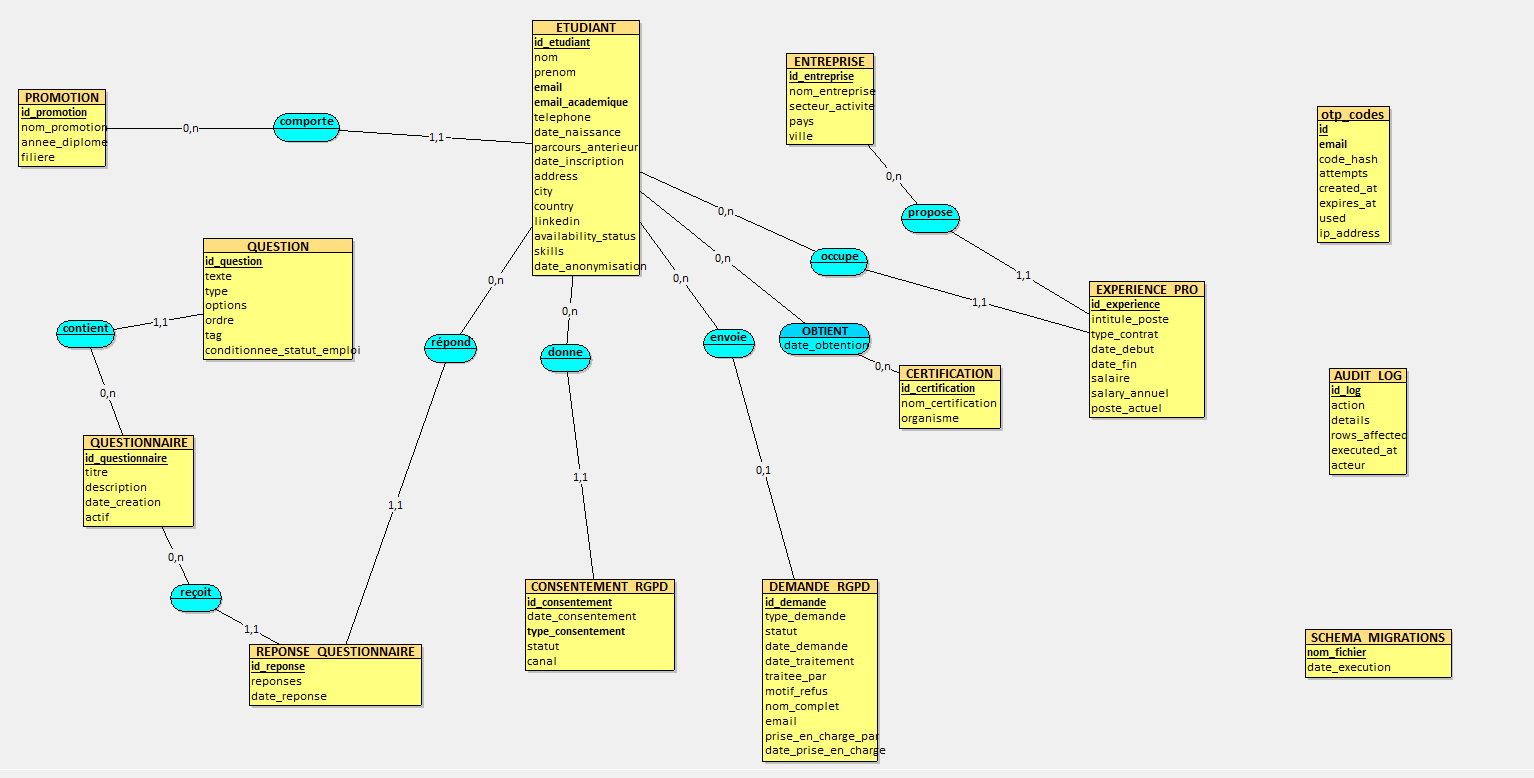
\includegraphics[width=\textwidth,keepaspectratio]{MCD.png}
  \caption{Modèle Conceptuel de Données (MCD) : entités, associations et cardinalités du système Alumni CRM.}
  \label{fig:mcd}
\end{figure}

\begin{figure}[htbp]
  \centering
  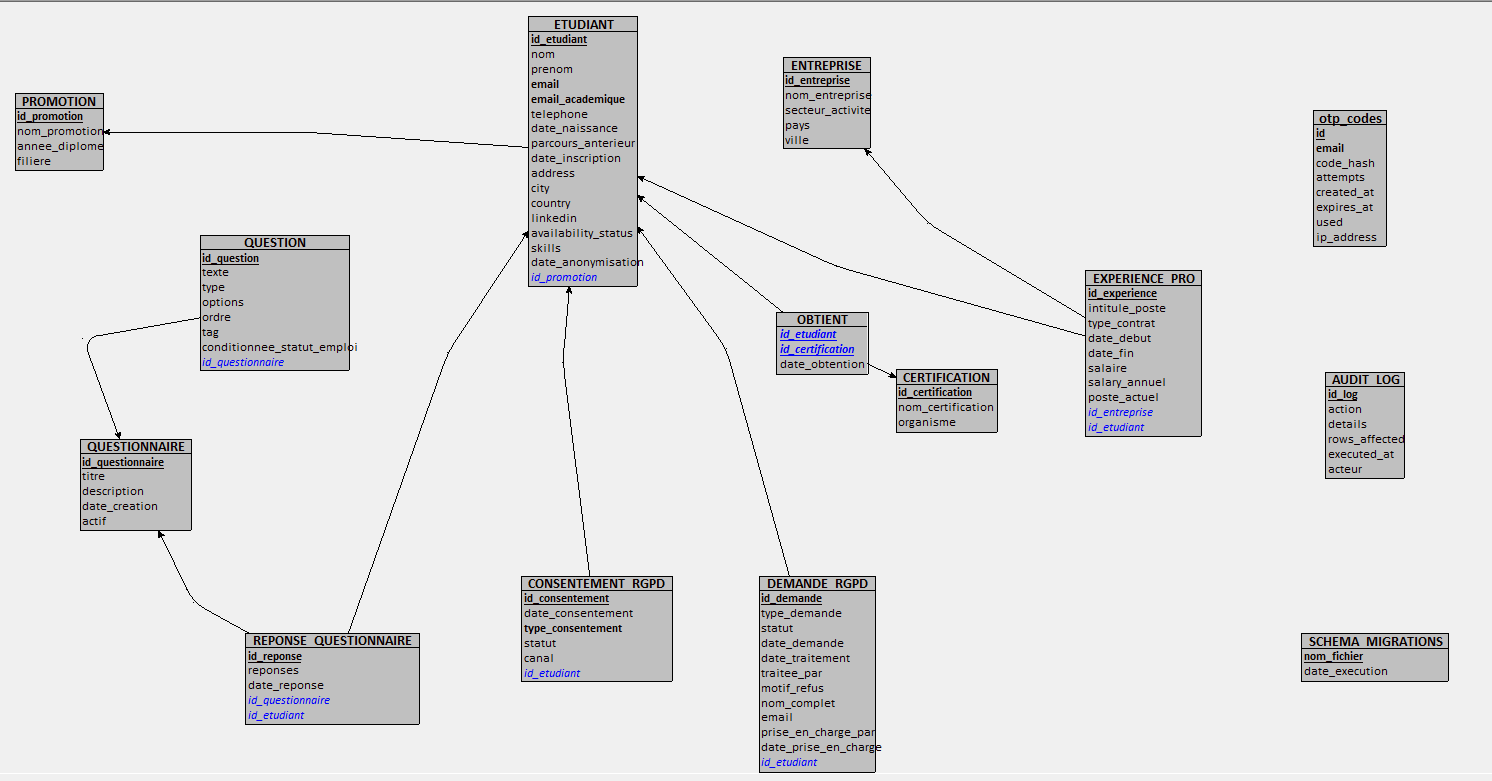
\includegraphics[width=\textwidth,keepaspectratio]{MLD.png}
  \caption{Modèle Logique de Données (MLD) : 14 tables relationnelles et leurs clés étrangères.}
  \label{fig:mld}
\end{figure}

\textbf{Vue d'ensemble des 14 tables et de leurs relations~:}

\begin{table}[htbp]
\centering
\caption{Vue d'ensemble des 14 tables par domaine fonctionnel.}
\label{tab:domaines-tables}
\rowcolors{2}{gray!8}{white}
\begin{tabularx}{\textwidth}{@{} l *{2}{>{\raggedright\arraybackslash}X} @{}}
\toprule
\textbf{Domaine} & \textbf{Tables} & \textbf{Relations principales} \\
\midrule
Données étudiantes & ETUDIANT, PROMOTION & ETUDIANT.id\_promotion $\rightarrow$ PROMOTION (N:1) \\
Parcours professionnel & ENTREPRISE, EXPERIENCE\_PRO, CERTIFICATION, OBTIENT & EXPERIENCE\_PRO $\rightarrow$ ETUDIANT et ENTREPRISE (N:1, avec \texttt{salary\_annuel NUMERIC})~; OBTIENT = association \hyperlink{abbr-NM}{N:M~(27)} ETUDIANT $\leftrightarrow$ CERTIFICATION \\
\hyperlink{abbr-RGPD}{RGPD~(40)} & CONSENTEMENT\_RGPD, DEMANDE\_RGPD, AUDIT\_LOG & CONSENTEMENT\_RGPD $\rightarrow$ ETUDIANT~; DEMANDE\_RGPD $\rightarrow$ ETUDIANT en SET NULL pour préserver l'historique après anonymisation~; AUDIT\_LOG journalise anonymisations, purges et nettoyages \\
Questionnaires & QUESTIONNAIRE, QUESTION, REPONSE\_QUESTIONNAIRE & QUESTION $\rightarrow$ QUESTIONNAIRE (N:1, avec tags \hyperlink{abbr-KPI}{KPI~(23)})~; REPONSE\_QUESTIONNAIRE $\rightarrow$ ETUDIANT + QUESTIONNAIRE (réponses stockées en \hyperlink{abbr-JSON}{JSON~(20)}) \\
Infrastructure & otp\_codes, schema\_migrations & otp\_codes~: codes \hyperlink{abbr-OTP}{OTP~(28)} hachés identifiés par l'email~; schema\_migrations~: suivi des migrations versionnées (17 fichiers) \\
\bottomrule
\end{tabularx}
\end{table}

\textbf{Règles d'intégrité}~: clés étrangères avec \hyperlink{abbr-CASCADE}{CASCADE~(2)} sur les données dépendant d'un étudiant (expériences, certifications obtenues, consentements, réponses), SET NULL sur les demandes \hyperlink{abbr-RGPD}{RGPD~(40)}, contraintes d'unicité (ex. email étudiant), contraintes \hyperlink{abbr-CHECK}{CHECK~(3)} sur les énumérations (statuts de demande \hyperlink{abbr-RGPD}{RGPD~(40)}, types de consentement).

\chapter{Interface de connexion}

L'alumni \hyperlink{abbr-CRM}{CRM~(5)} propose deux modes d'authentification~: un accès administrateur par code et une connexion alumni par \hyperlink{abbr-OTP}{OTP~(28)} (code à 6 chiffres envoyé par email). L'interface supporte le thème clair et le thème sombre (dark mode), activé par le bouton en haut à droite de la page de connexion.

\begin{figure}[htbp]
  \centering
  \begin{minipage}{0.48\textwidth}
    \centering
    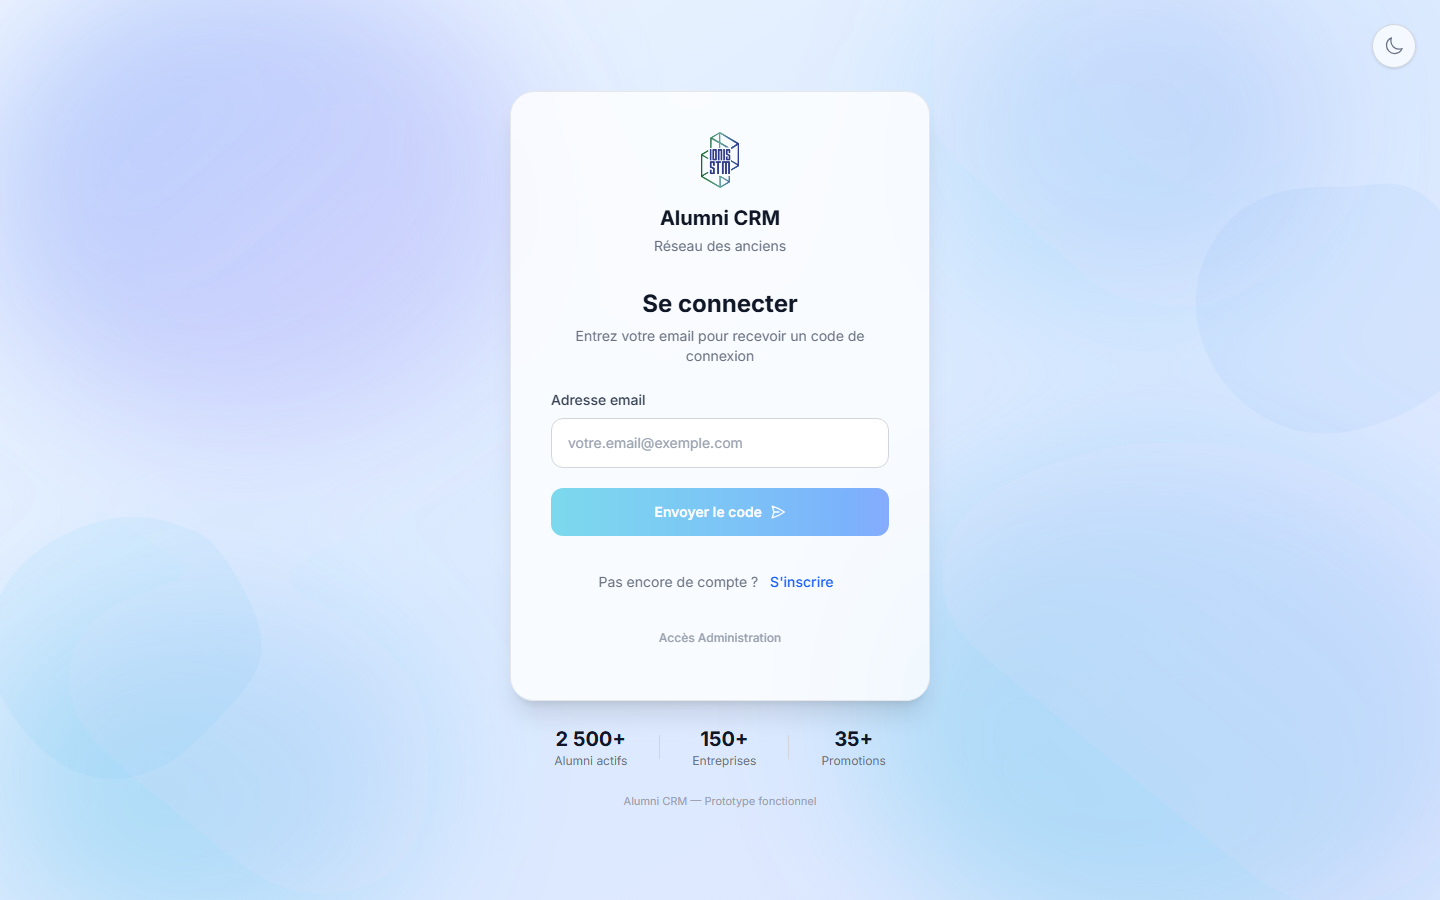
\includegraphics[width=\textwidth]{login_light.png}
    \caption{Mode clair.}
  \end{minipage}\hfill
  \begin{minipage}{0.48\textwidth}
    \centering
    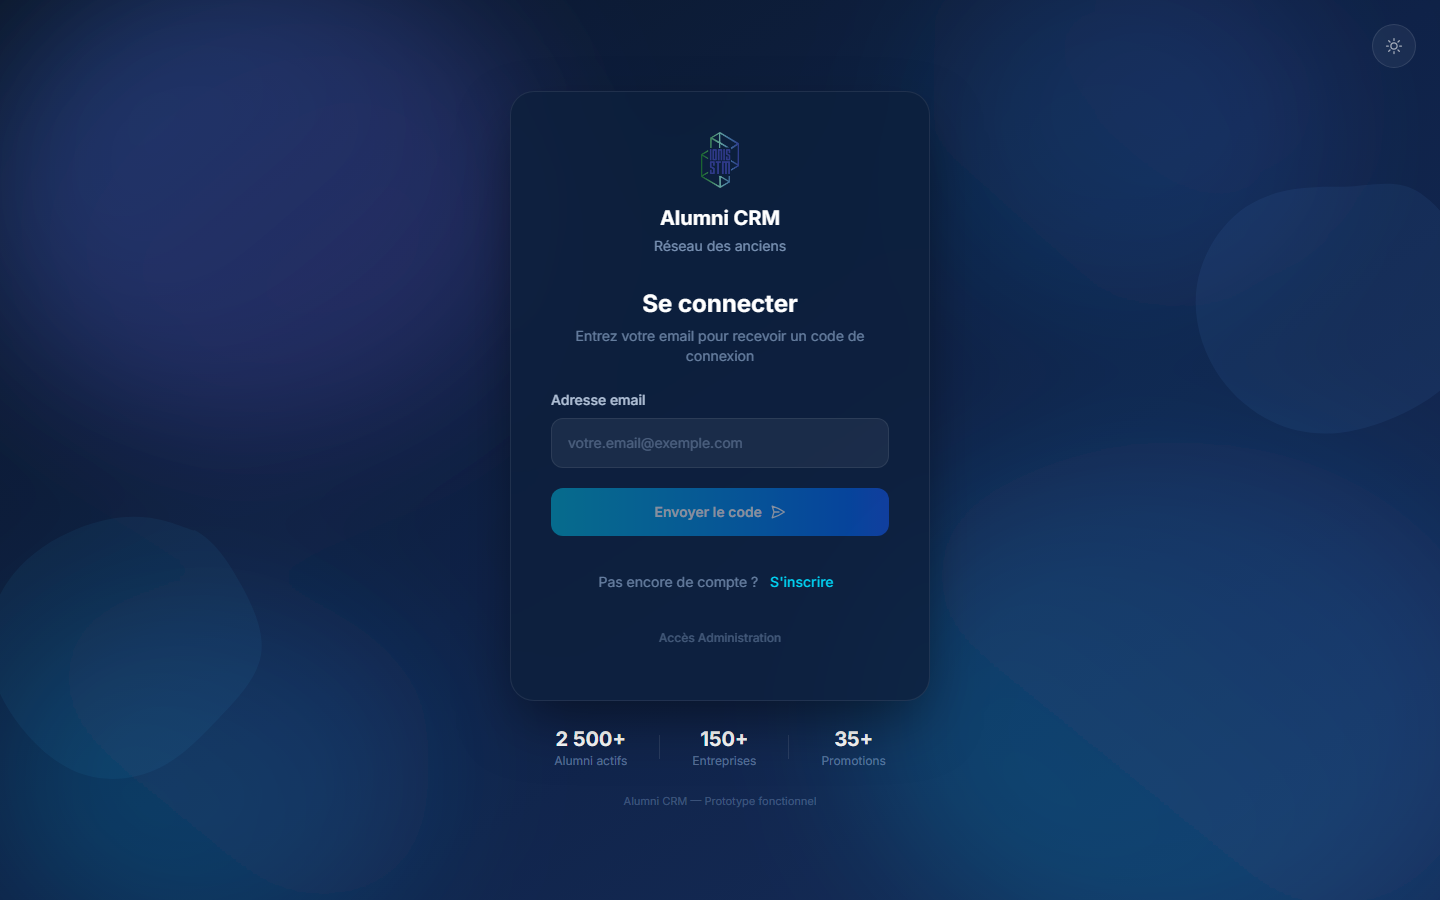
\includegraphics[width=\textwidth]{login_dark.png}
    \caption{Mode sombre.}
  \end{minipage}
  \caption{Page de connexion -- thème clair vs thème sombre.}
\end{figure}

\textbf{Connexion administrateur.} L'accès à l'espace administration se fait via un écran dédié de connexion par code d'accès, décliné en mode clair et sombre.

\begin{figure}[htbp]
  \centering
  \begin{minipage}{0.48\textwidth}
    \centering
    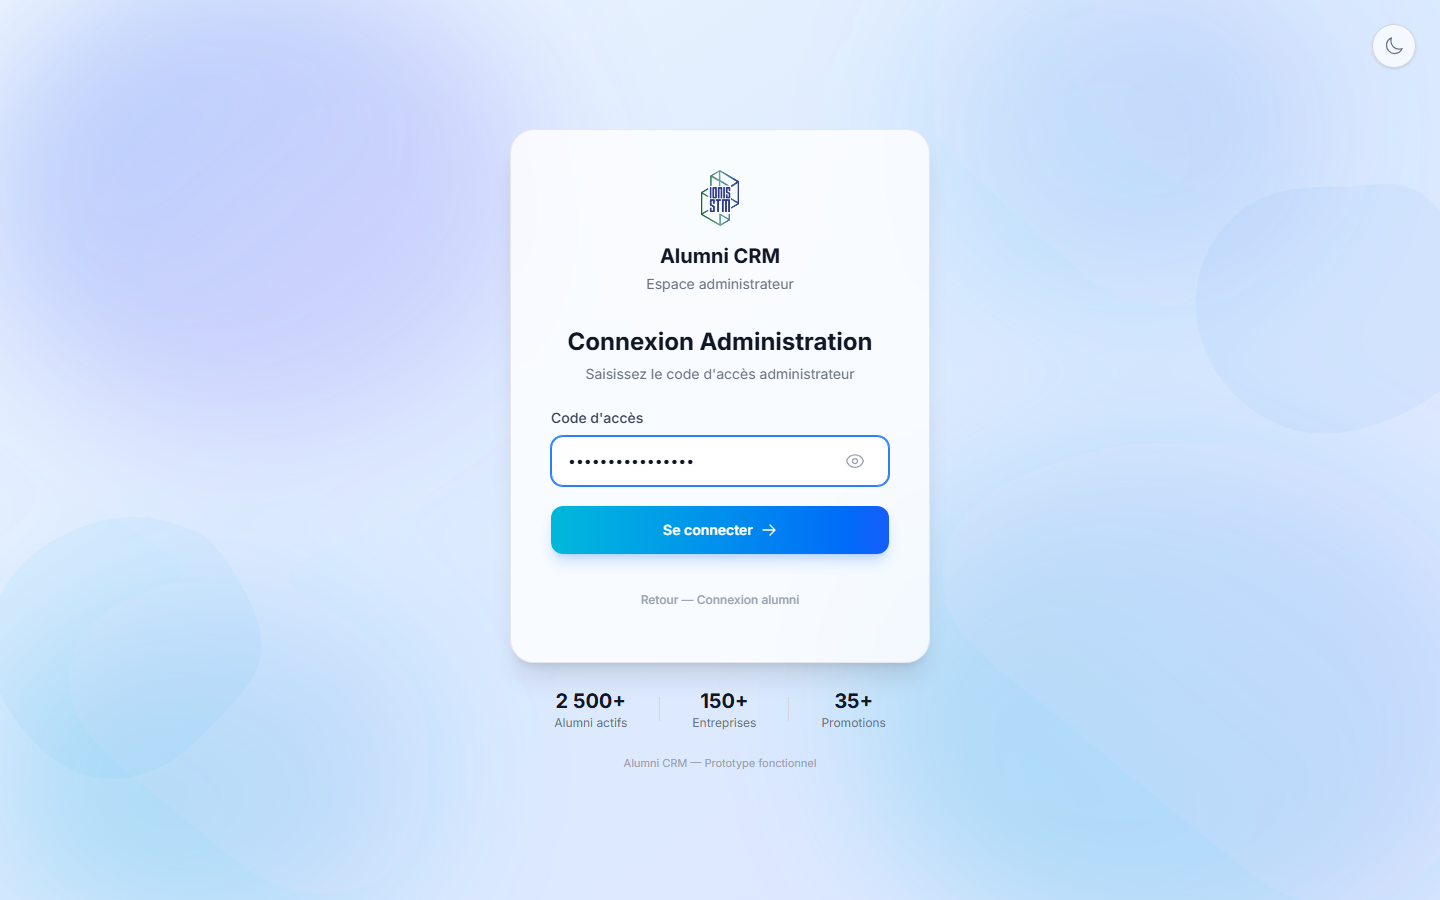
\includegraphics[width=\textwidth]{login_admin_light.png}
    \caption{Mode clair.}
  \end{minipage}\hfill
  \begin{minipage}{0.48\textwidth}
    \centering
    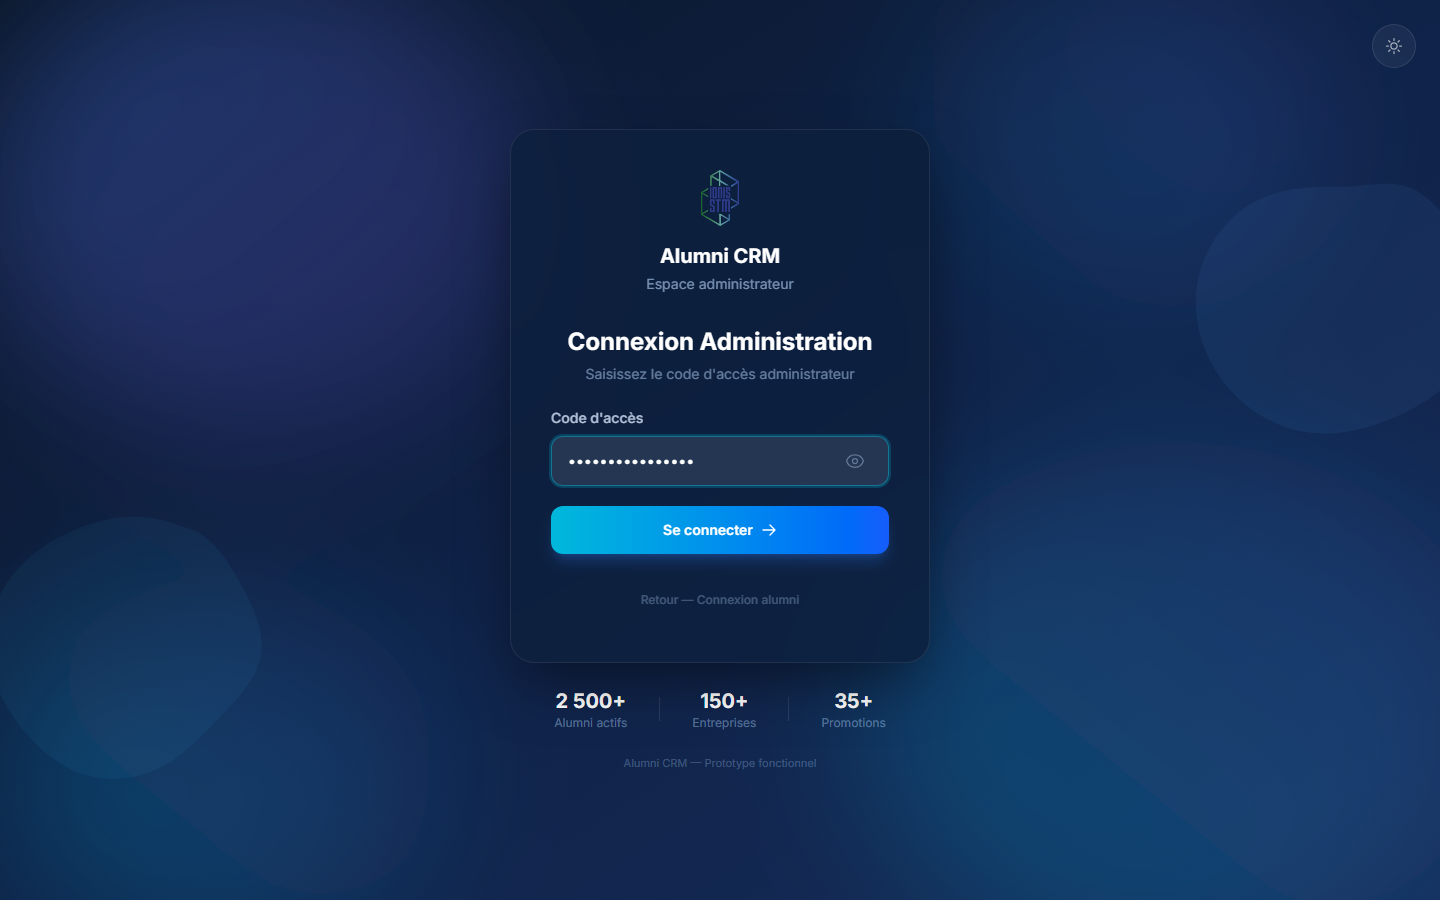
\includegraphics[width=\textwidth]{login_admin_dark.png}
    \caption{Mode sombre.}
  \end{minipage}
  \caption{Page de connexion administrateur (code d'accès) -- thème clair vs thème sombre.}
\end{figure}

\textbf{Vérification \hyperlink{abbr-OTP}{OTP~(28)}.} Après saisie de l'adresse email, un code à 6 chiffres est envoyé. La page de vérification présente une saisie animée du code~; en cas de code incorrect, un message d'erreur s'affiche avec le nombre de tentatives restantes.

\begin{figure}[htbp]
  \centering
  \begin{minipage}{0.48\textwidth}
    \centering
    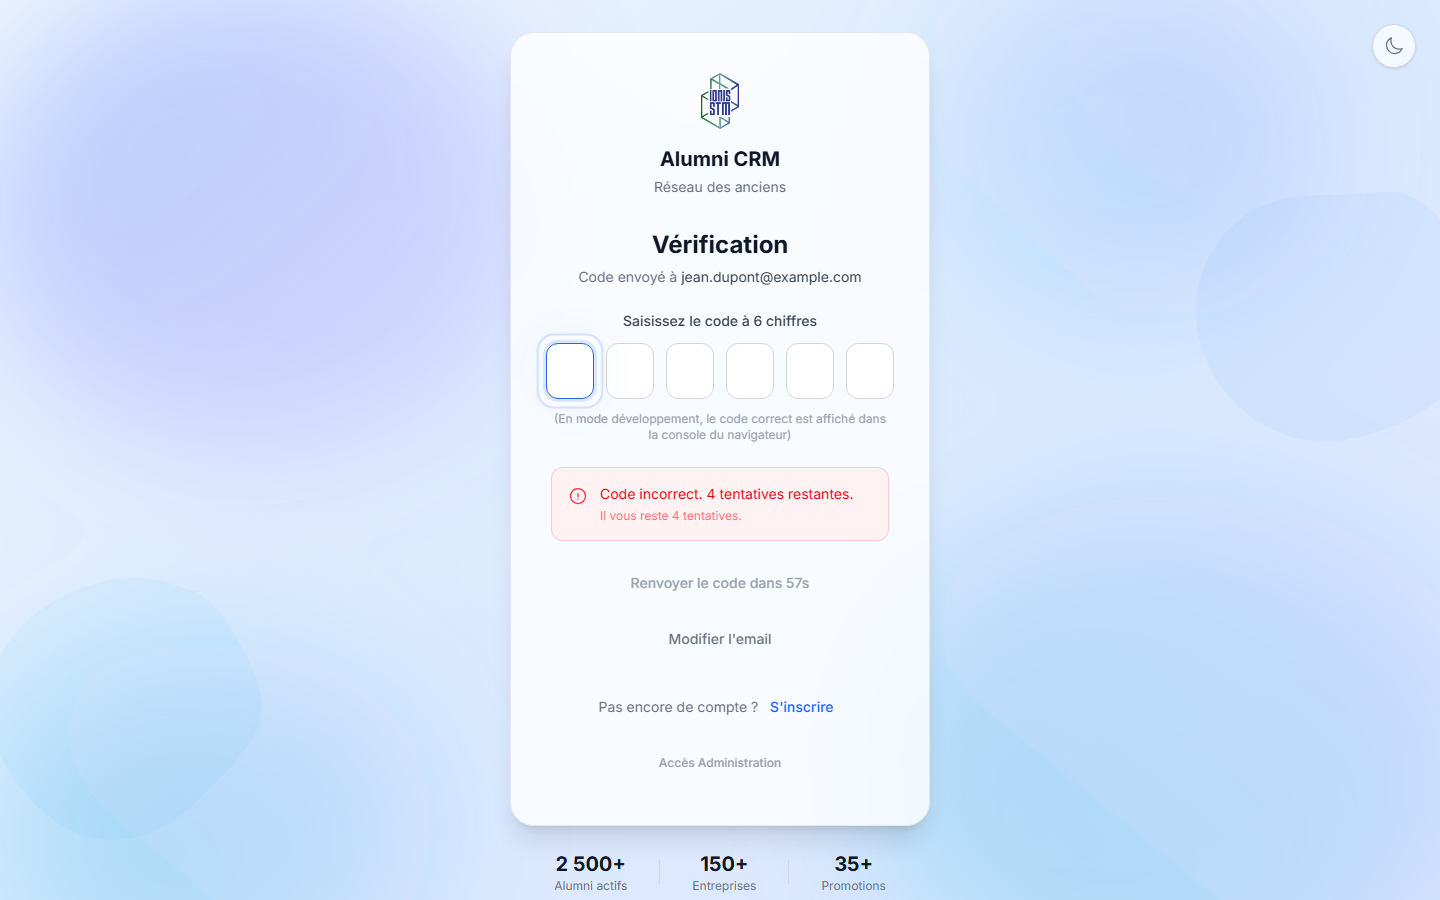
\includegraphics[width=\textwidth]{otp_error_light.png}
    \caption{Mode clair.}
  \end{minipage}\hfill
  \begin{minipage}{0.48\textwidth}
    \centering
    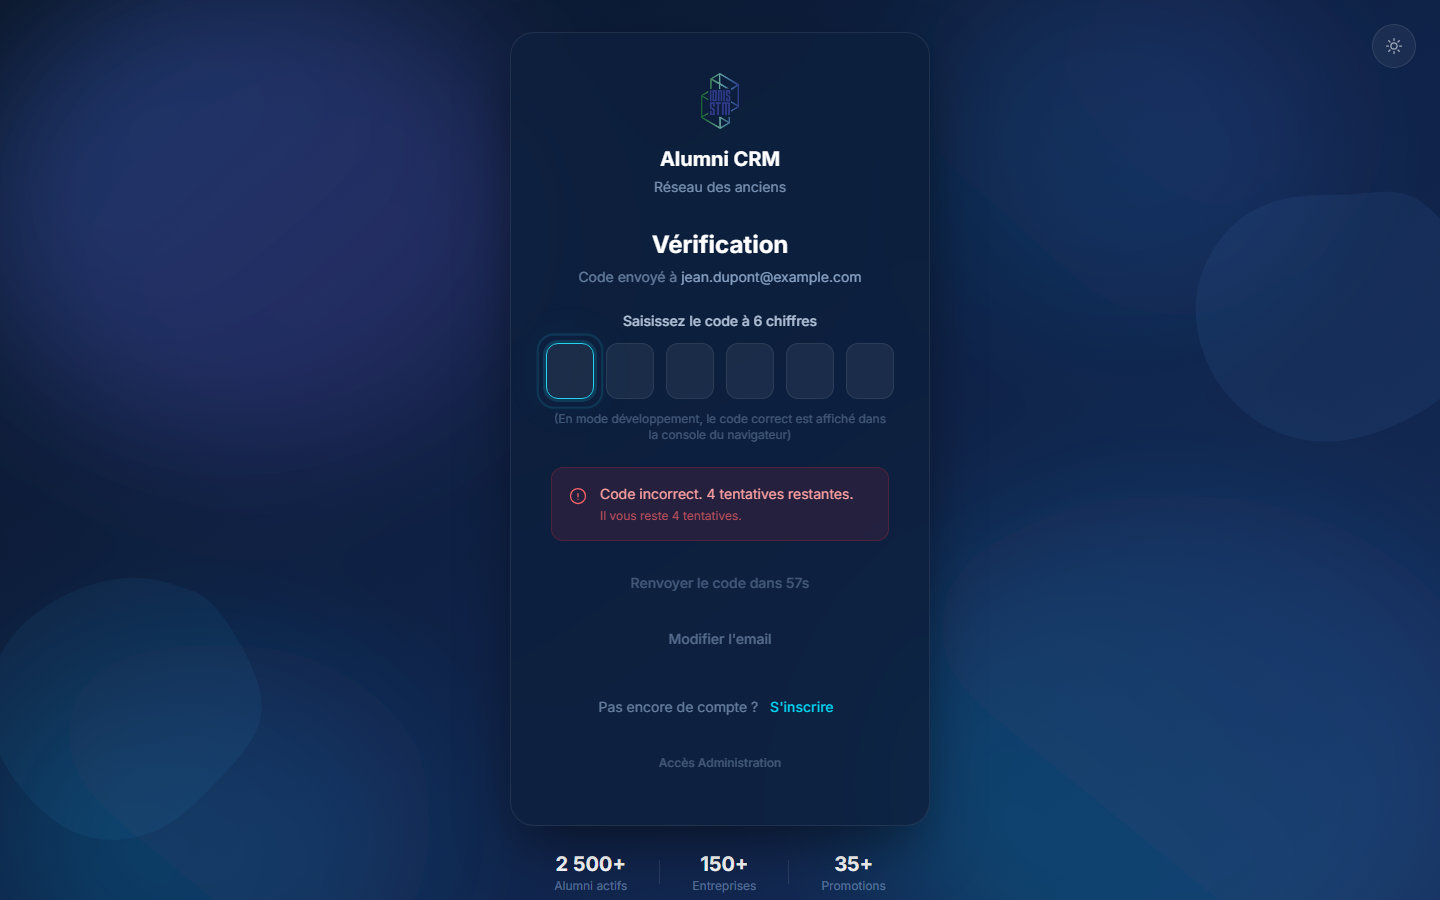
\includegraphics[width=\textwidth]{otp_error_dark.png}
    \caption{Mode sombre.}
  \end{minipage}
  \caption{Vérification OTP en erreur (code incorrect) -- thème clair vs thème sombre.}
\end{figure}

En cas de code valide, l'interface confirme le succès de la vérification avant la redirection vers l'espace alumni.

\begin{figure}[htbp]
  \centering
  \begin{minipage}{0.48\textwidth}
    \centering
    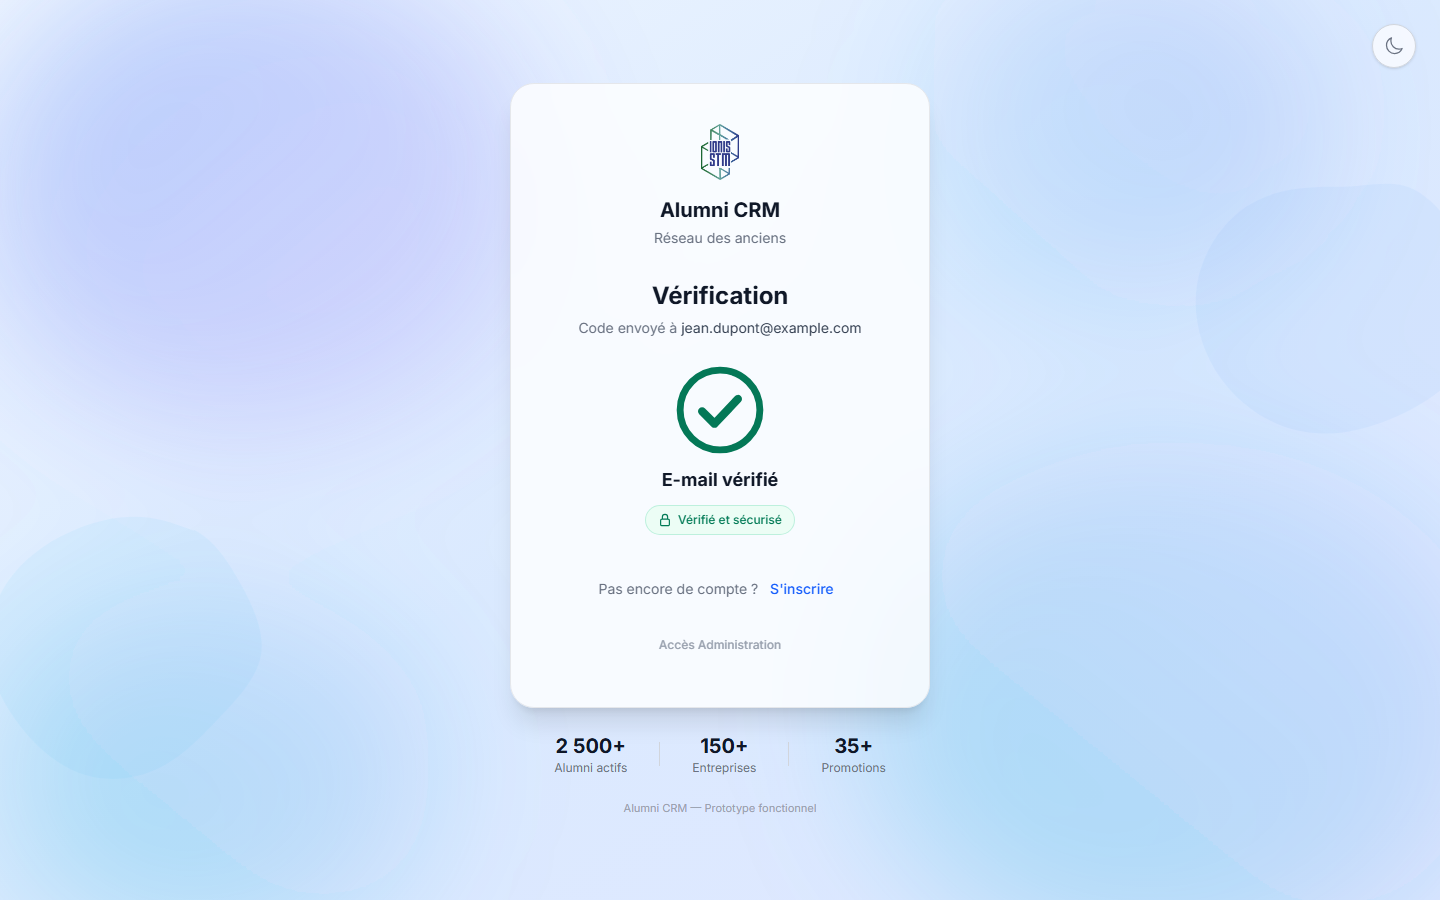
\includegraphics[width=\textwidth]{otp_success_light.png}
    \caption{Mode clair.}
  \end{minipage}\hfill
  \begin{minipage}{0.48\textwidth}
    \centering
    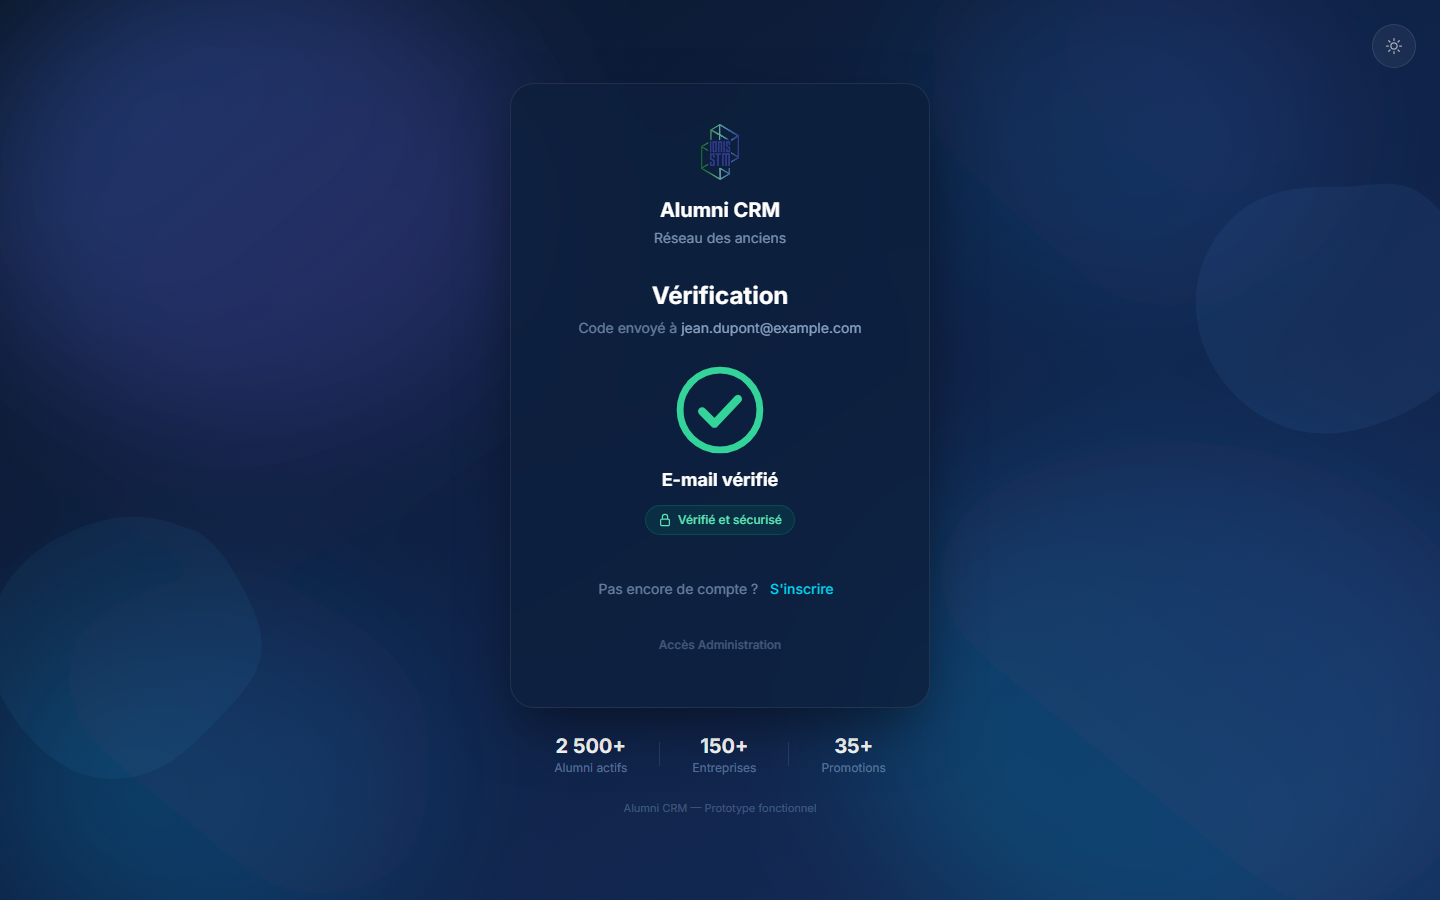
\includegraphics[width=\textwidth]{otp_success_dark.png}
    \caption{Mode sombre.}
  \end{minipage}
  \caption{Vérification OTP réussie (E-mail vérifié) -- thème clair vs thème sombre.}
\end{figure}

\chapter{Dashboard administrateur (captures d'écran)}

Les captures d'écran présentent le tableau de bord administrateur~: bento grid de \hyperlink{abbr-KPI}{KPI~(23)}, indicateurs, annuaire filtrable, traitement des demandes \hyperlink{abbr-RGPD}{RGPD~(40)}, gestion des promotions, gestion des questionnaires et import Excel. Chaque écran est présenté en mode clair et mode sombre.

\begin{figure}[htbp]
  \centering
  \begin{minipage}{0.48\textwidth}
    \centering
    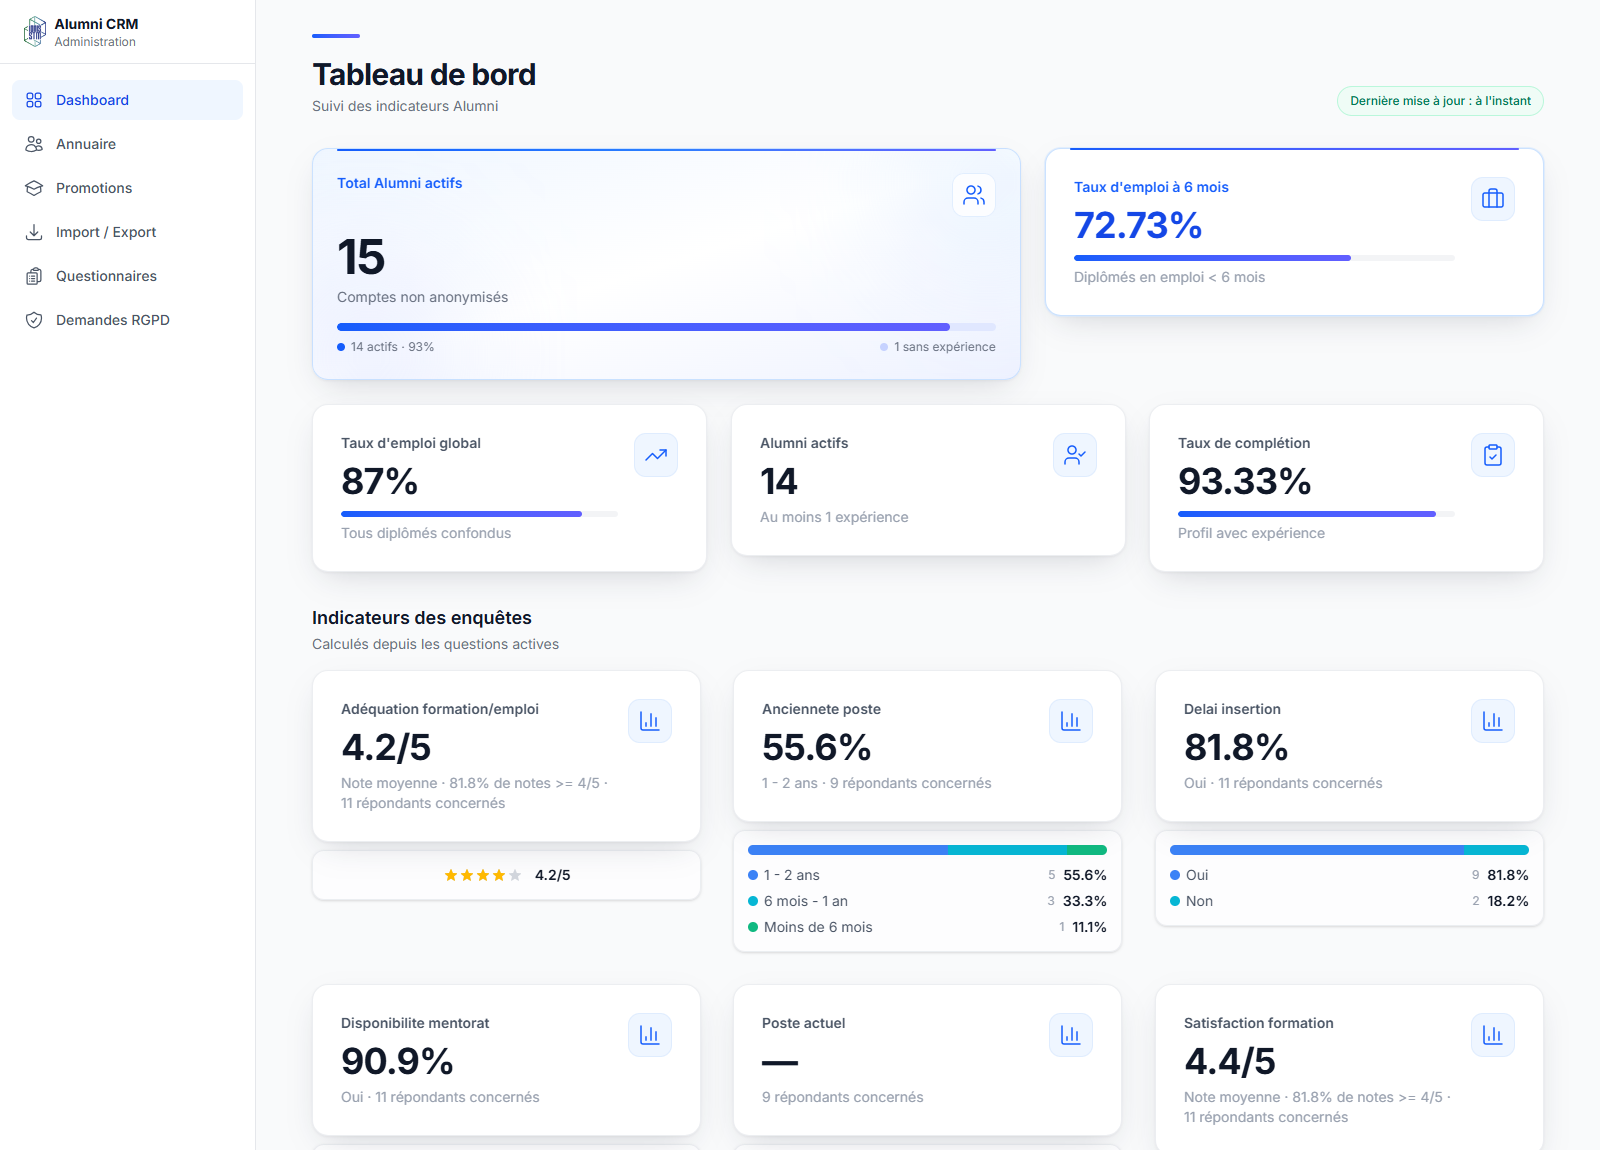
\includegraphics[width=\textwidth]{anB_dashboard_light_1.png}
    \caption{Mode clair -- partie 1/3.}
  \end{minipage}\hfill
  \begin{minipage}{0.48\textwidth}
    \centering
    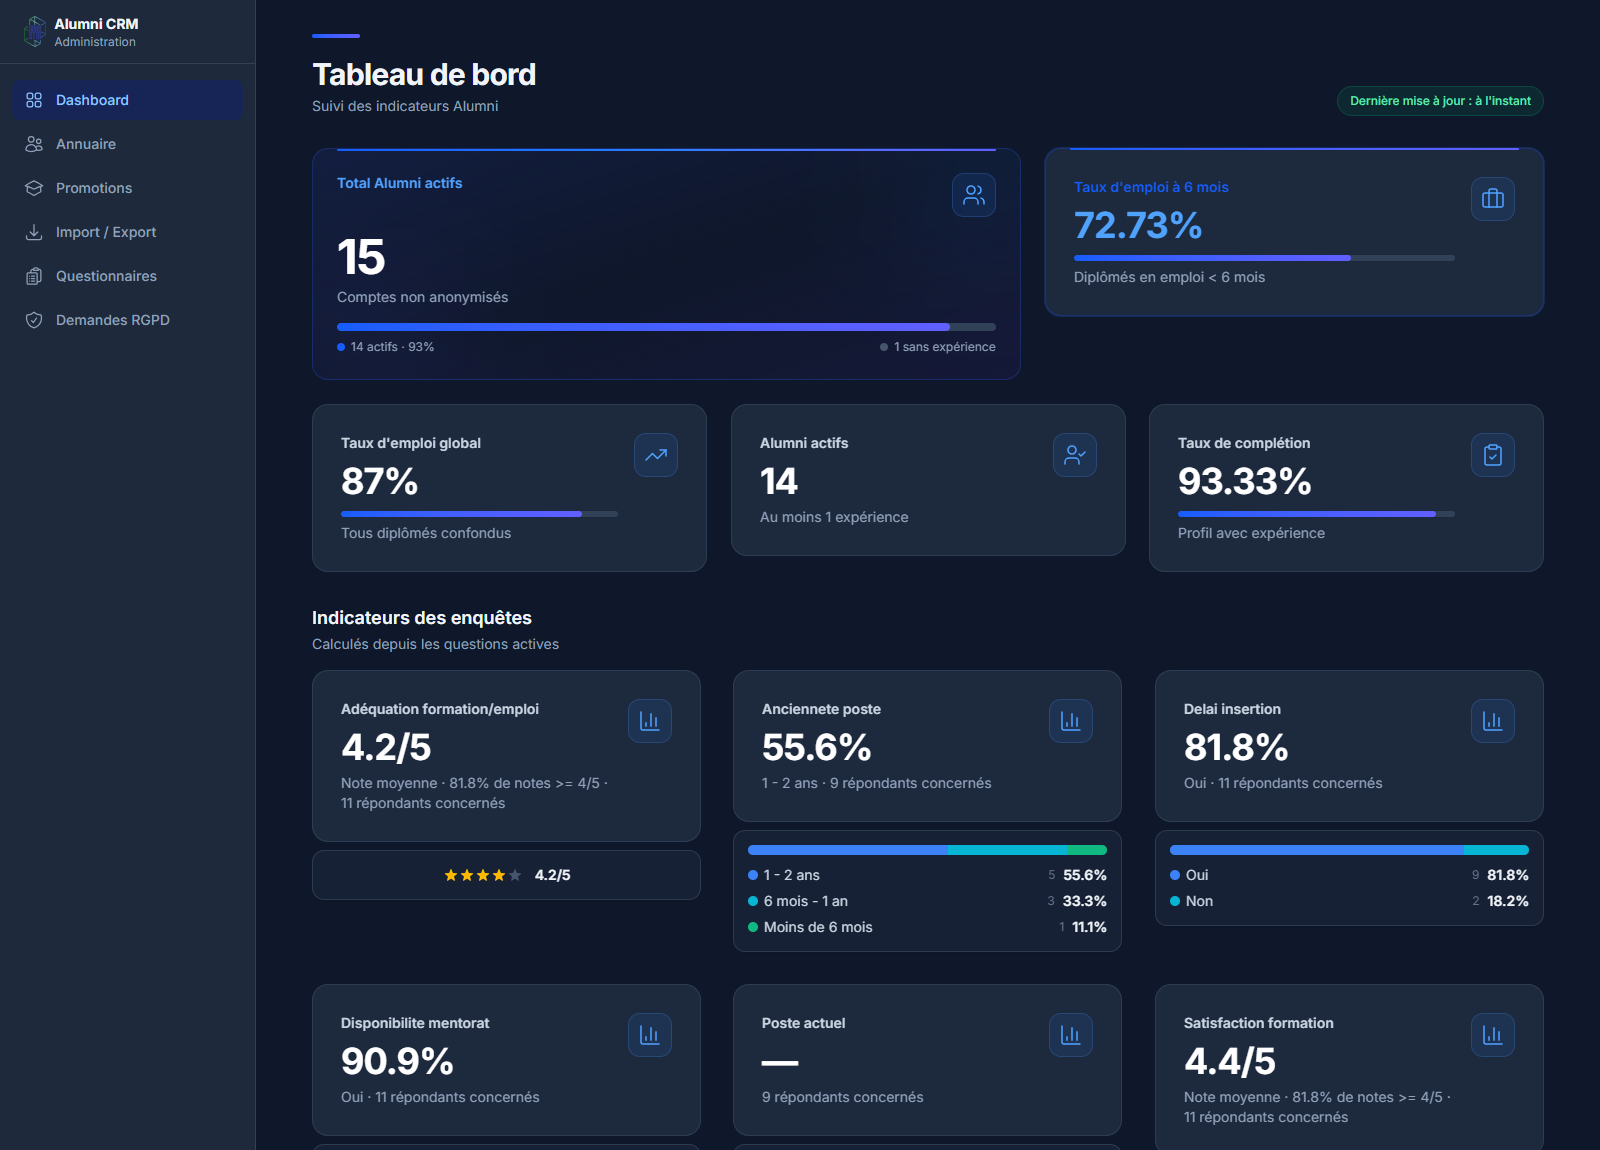
\includegraphics[width=\textwidth]{anB_dashboard_dark_1.png}
    \caption{Mode sombre -- partie 1/3.}
  \end{minipage}

  \medskip

  \begin{minipage}{0.48\textwidth}
    \centering
    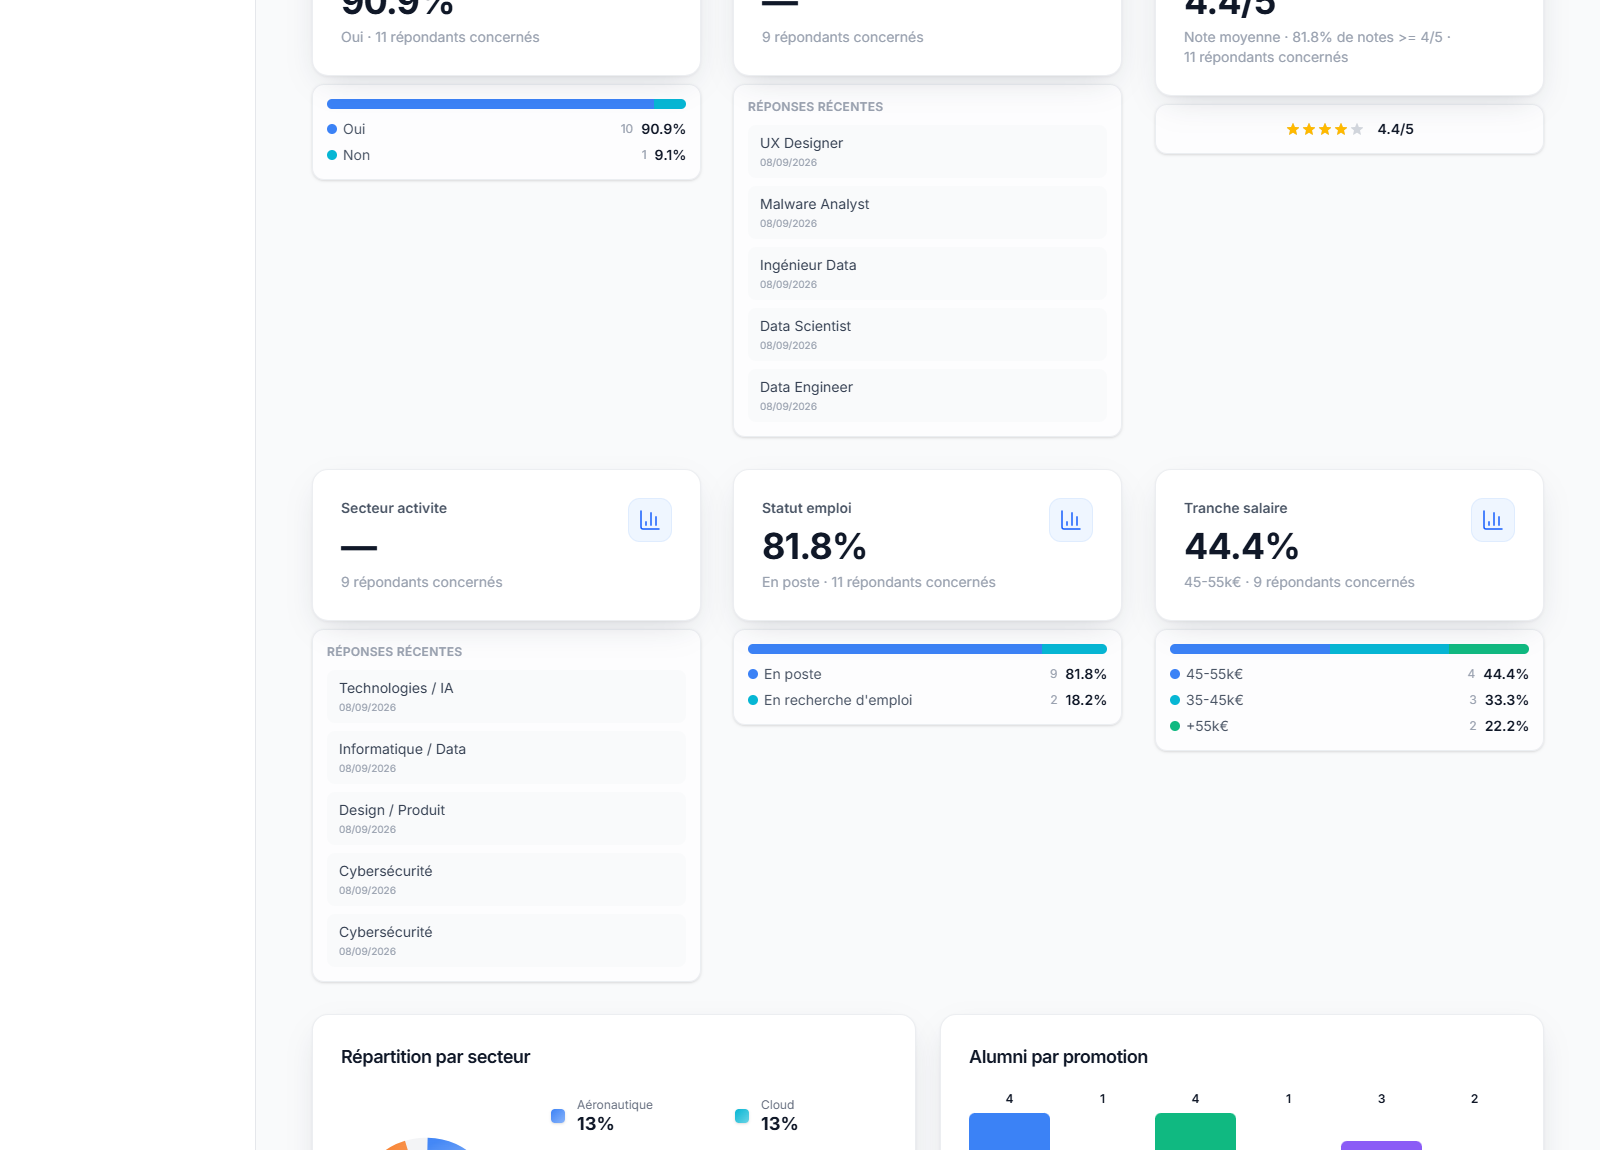
\includegraphics[width=\textwidth]{anB_dashboard_light_2.png}
    \caption{Mode clair -- partie 2/3.}
  \end{minipage}\hfill
  \begin{minipage}{0.48\textwidth}
    \centering
    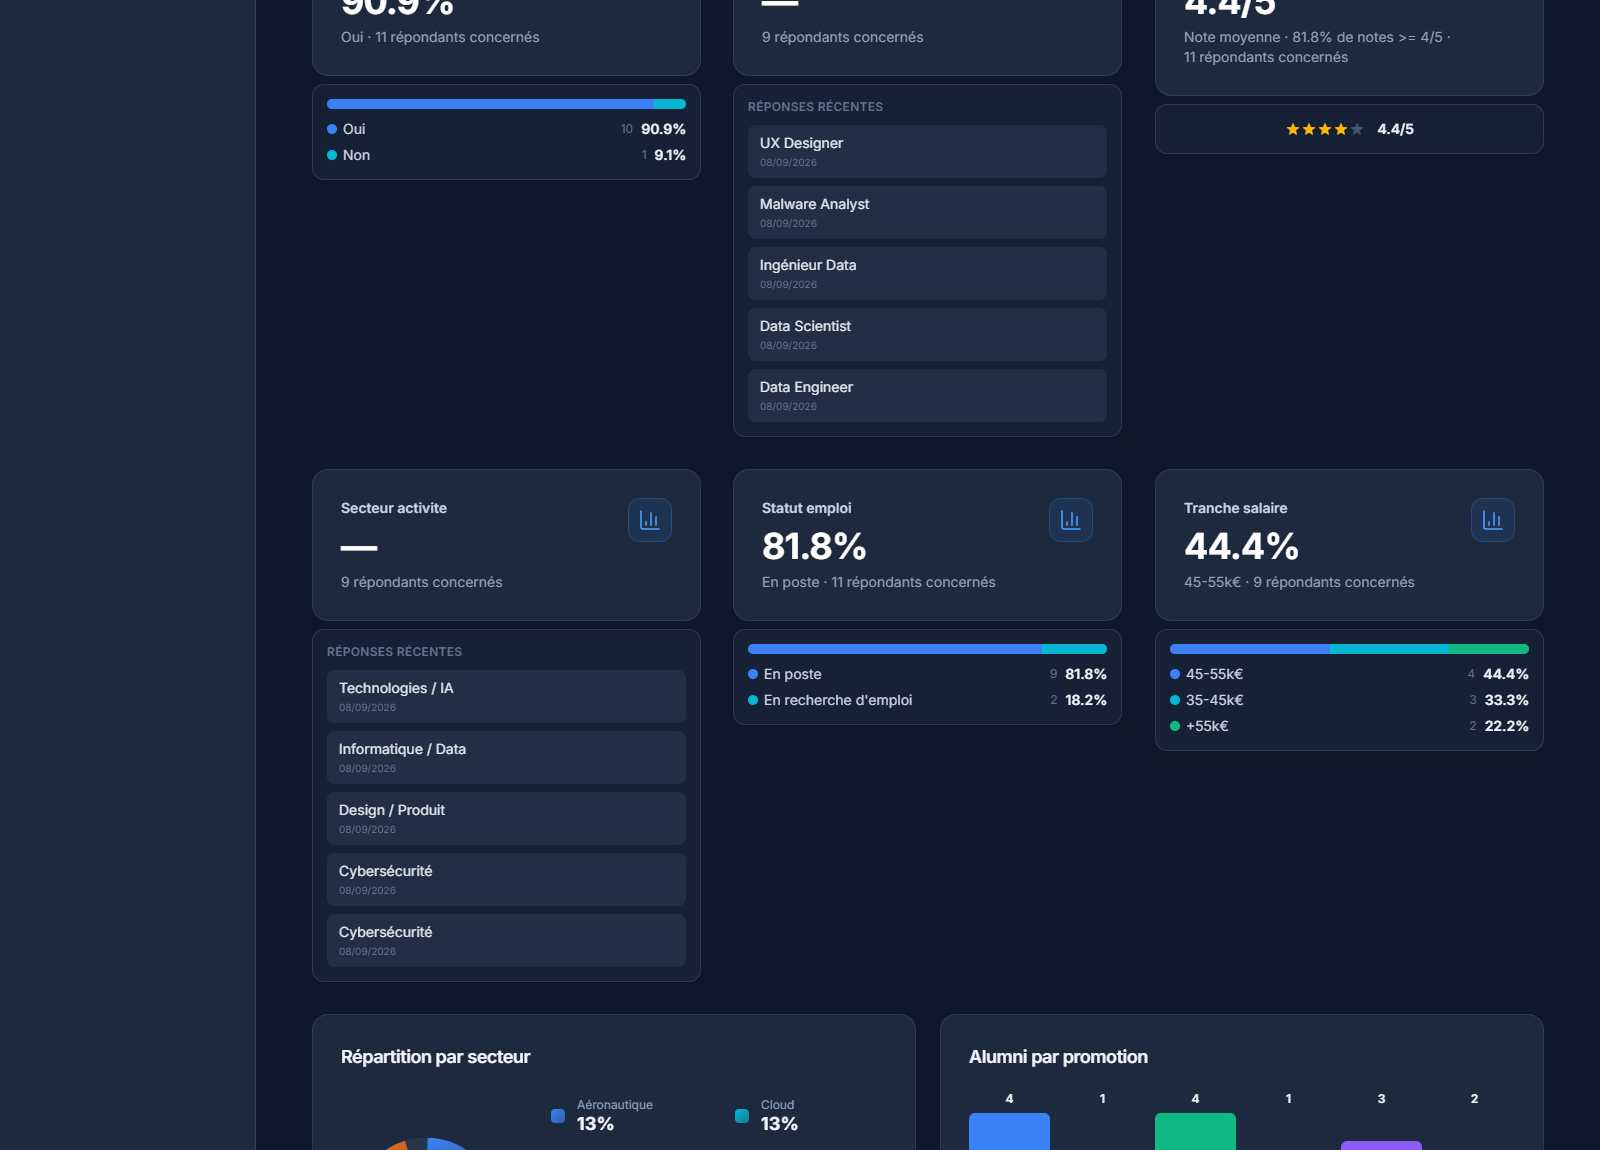
\includegraphics[width=\textwidth]{anB_dashboard_dark_2.png}
    \caption{Mode sombre -- partie 2/3.}
  \end{minipage}

  \medskip

  \begin{minipage}{0.48\textwidth}
    \centering
    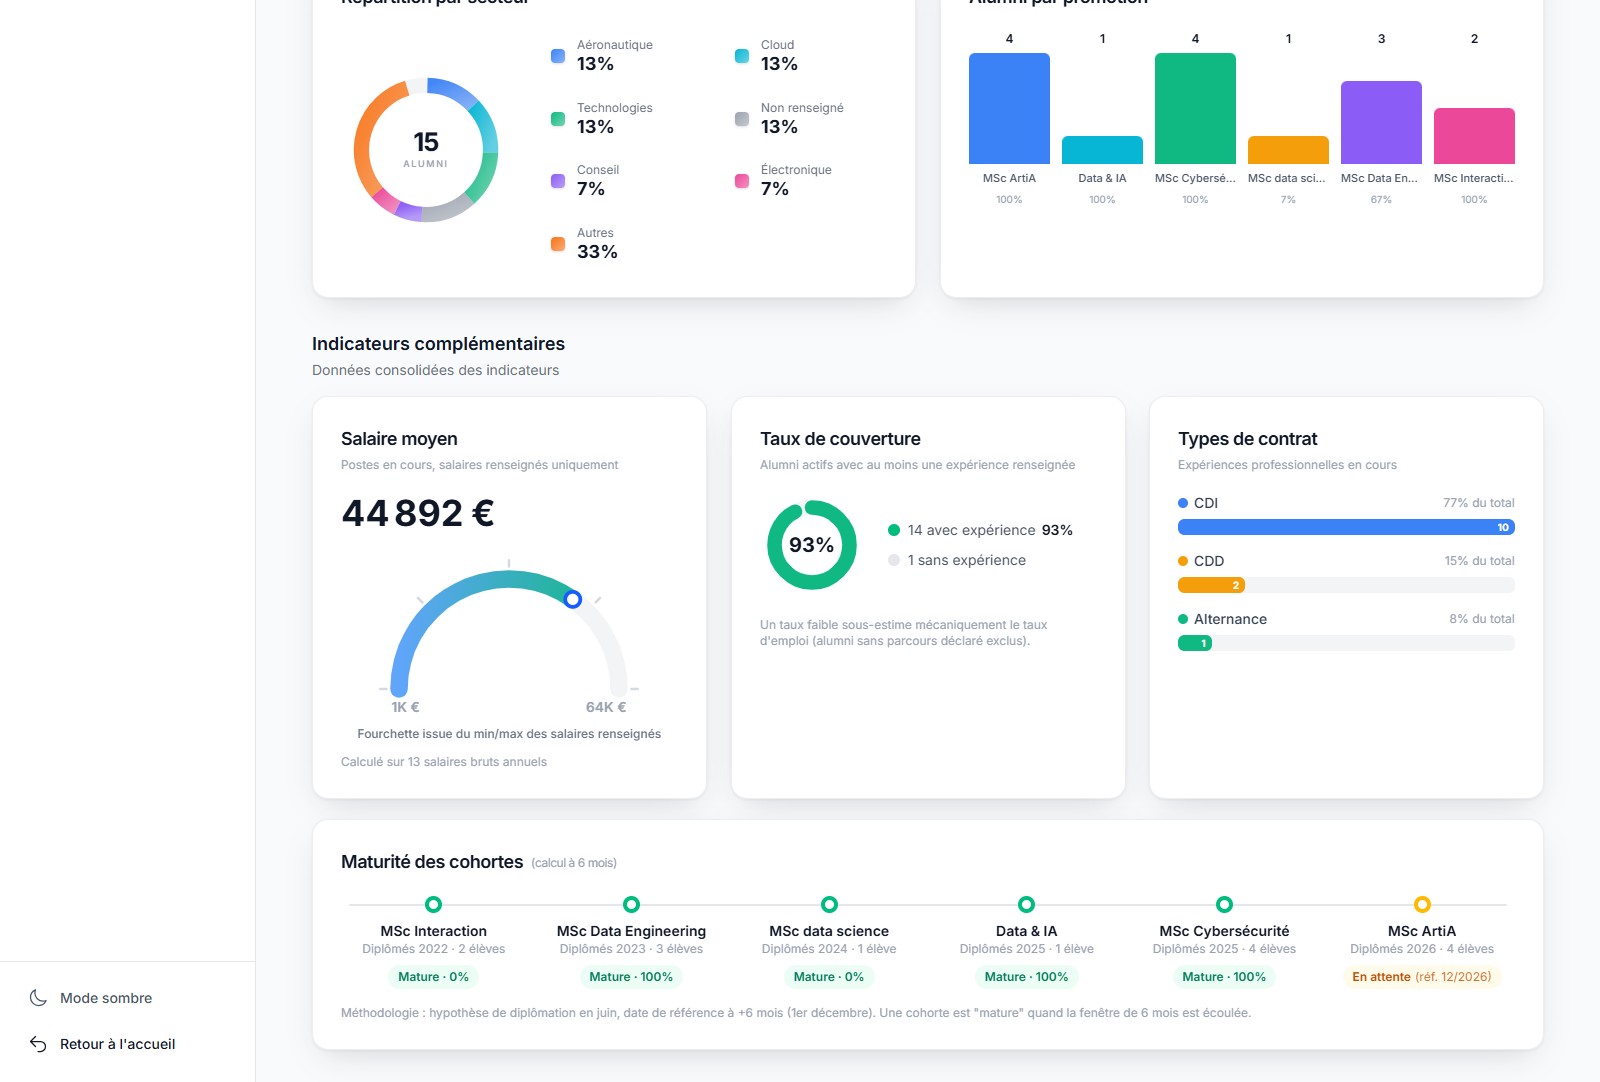
\includegraphics[width=\textwidth]{anB_dashboard_light_3.png}
    \caption{Mode clair -- partie 3/3.}
  \end{minipage}\hfill
  \begin{minipage}{0.48\textwidth}
    \centering
    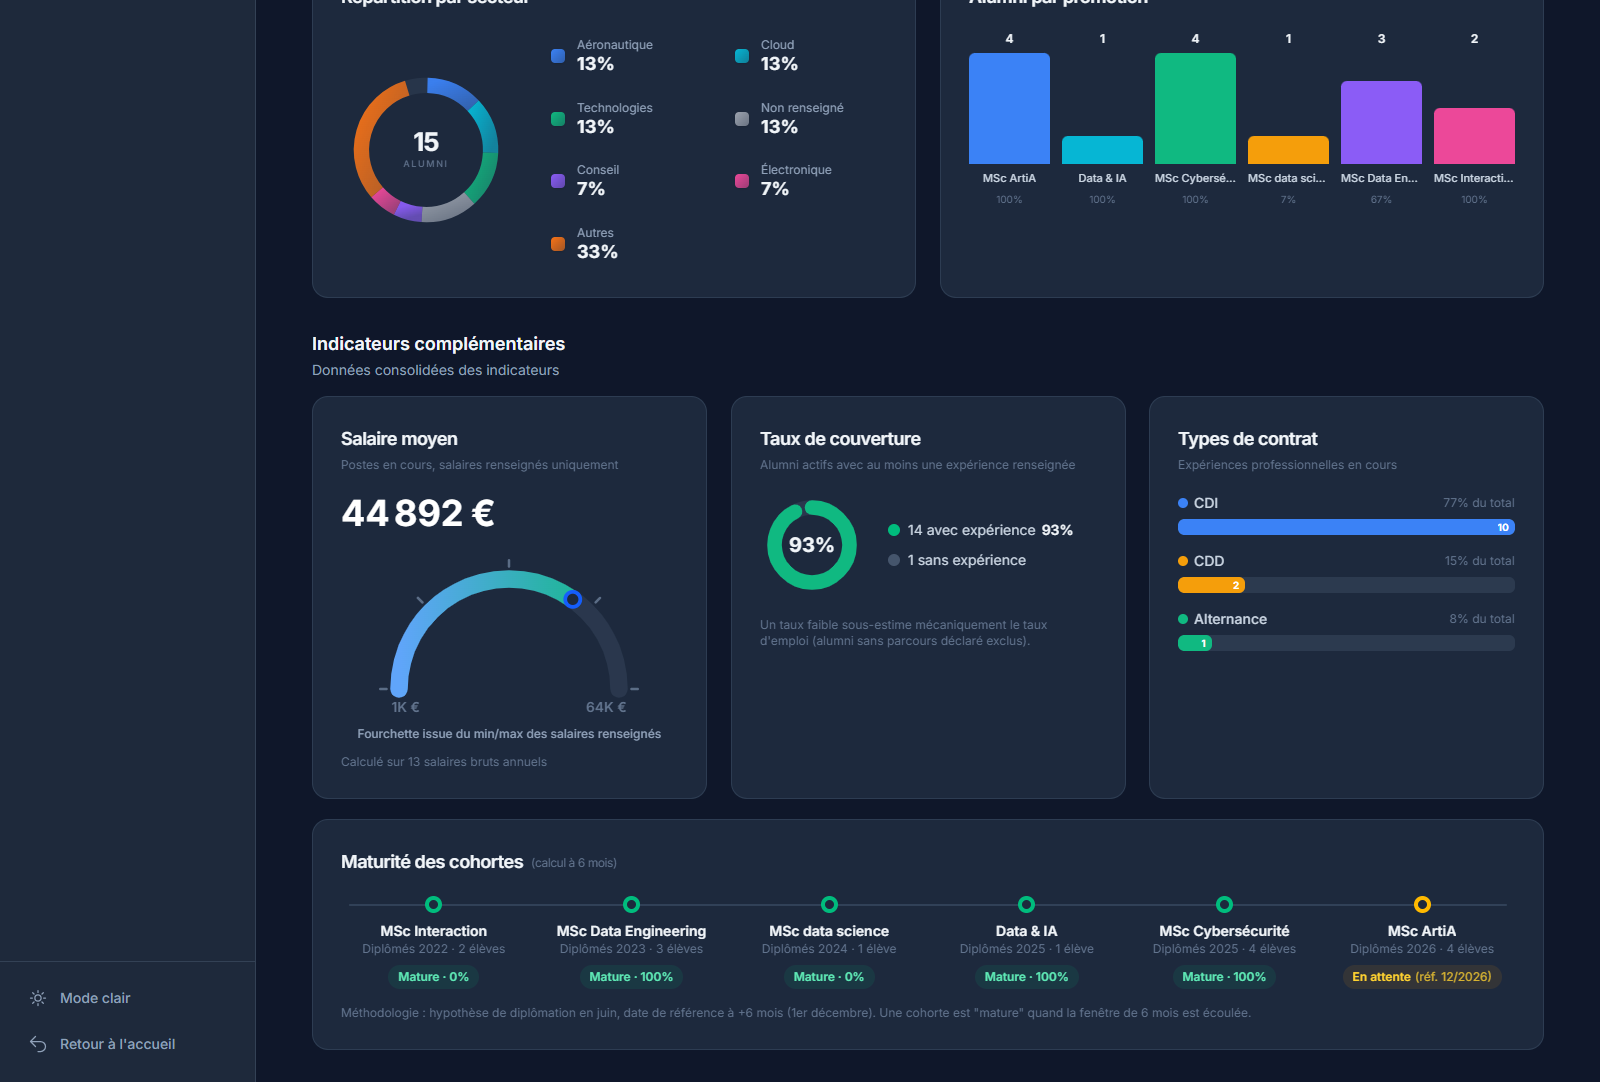
\includegraphics[width=\textwidth]{anB_dashboard_dark_3.png}
    \caption{Mode sombre -- partie 3/3.}
  \end{minipage}
  \caption{Tableau de bord administrateur (KPI, indicateurs, bento grid) -- thème clair vs thème sombre, capture intégrale en trois parties.}
\end{figure}

\begin{figure}[htbp]
  \centering
  \begin{minipage}{0.48\textwidth}
    \centering
    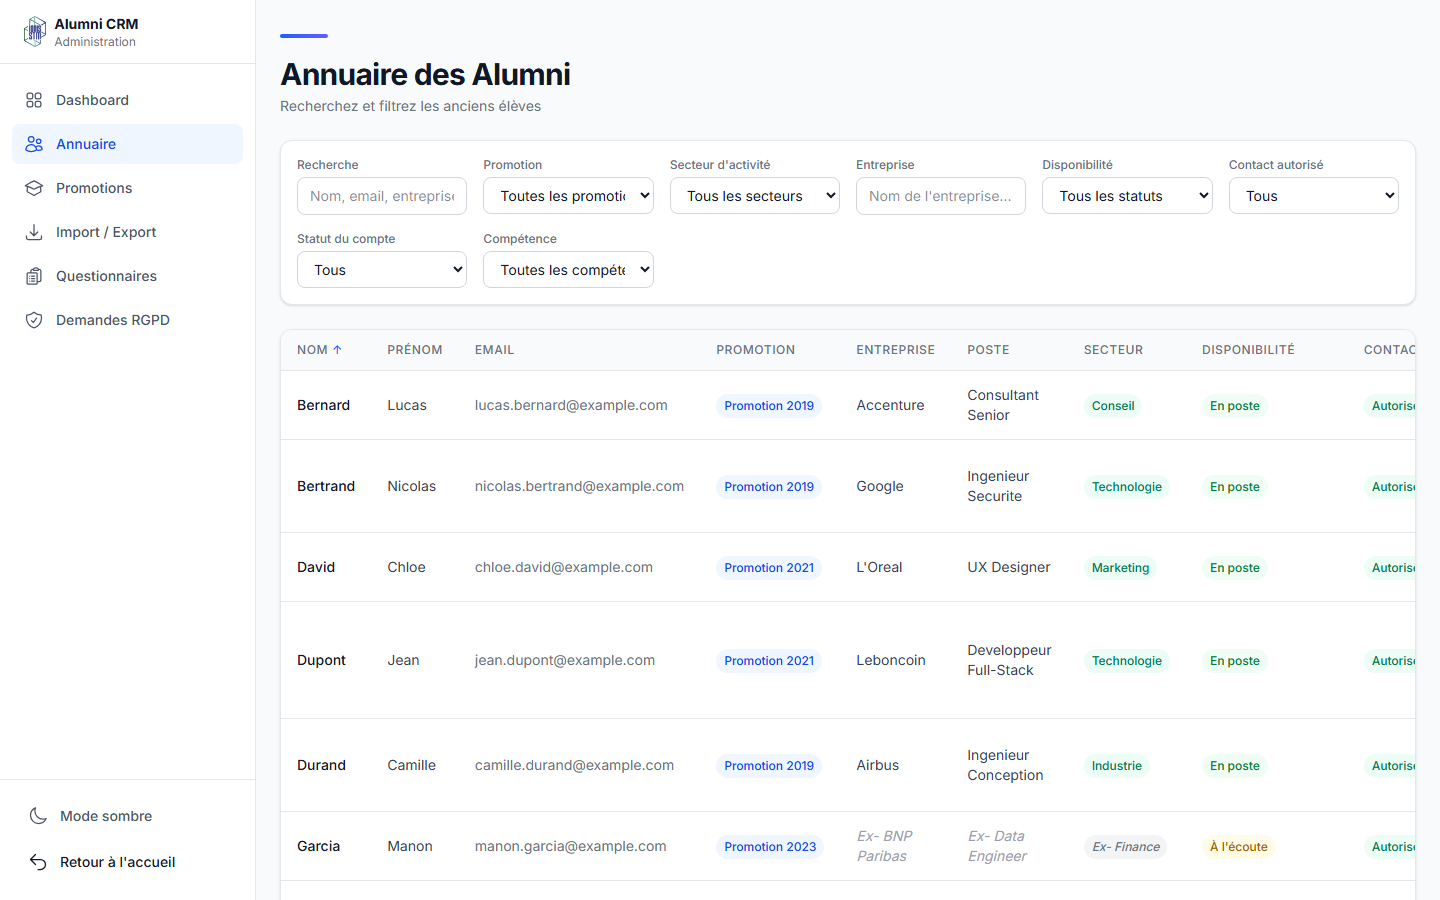
\includegraphics[width=\textwidth]{anB_annuaire_light.png}
    \caption{Mode clair.}
  \end{minipage}\hfill
  \begin{minipage}{0.48\textwidth}
    \centering
    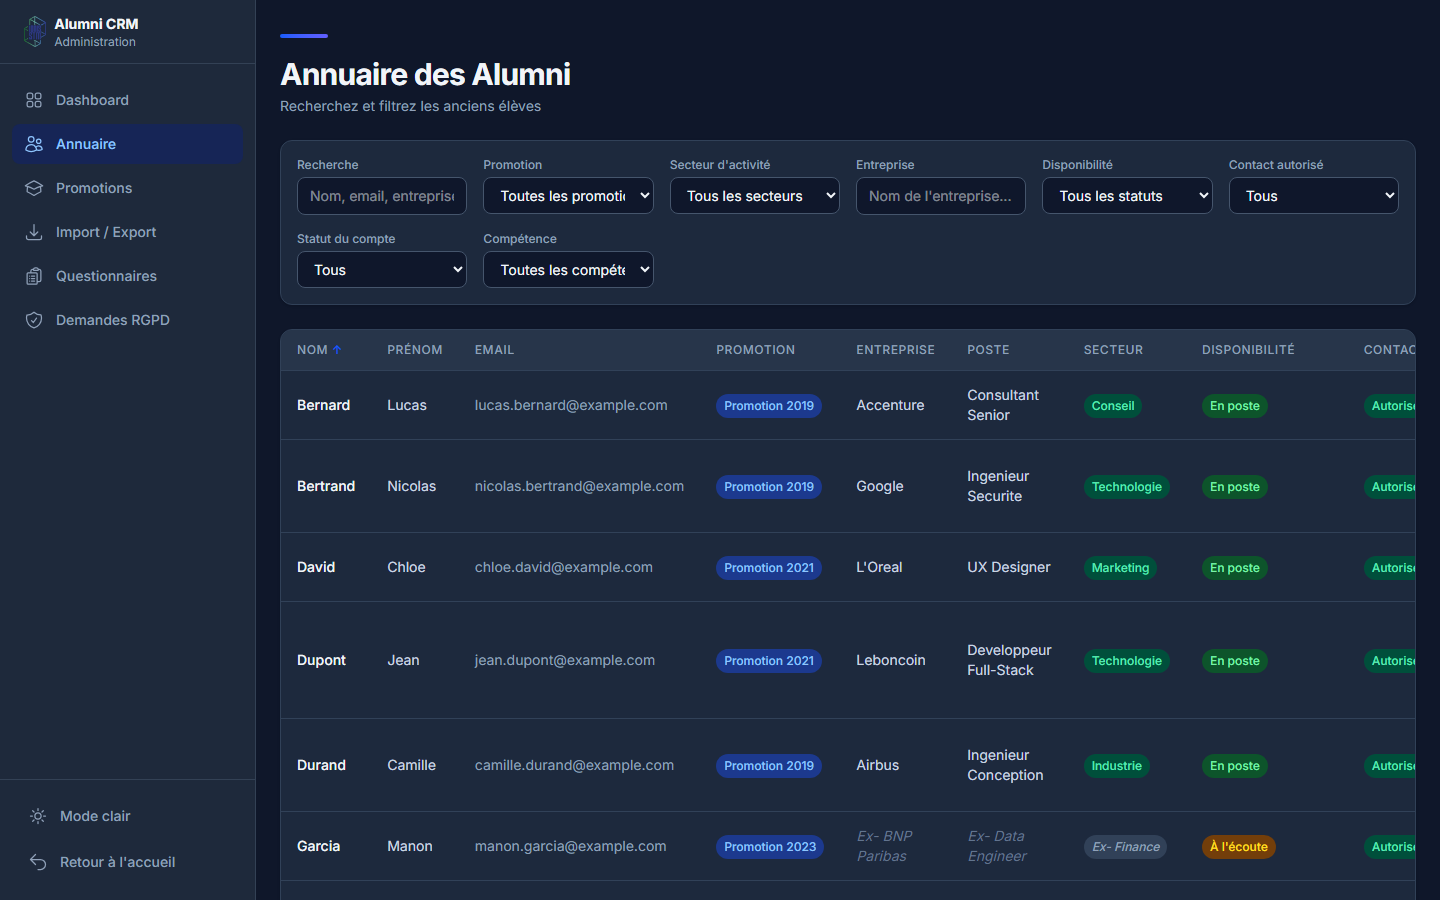
\includegraphics[width=\textwidth]{anB_annuaire_dark.png}
    \caption{Mode sombre.}
  \end{minipage}
  \caption{Annuaire des alumni filtrable (12 colonnes : promotion, secteur, entreprise, disponibilité, compétences, actions) -- thème clair vs thème sombre, capture intégrale (lignes et colonnes complètes).}
\end{figure}

\begin{figure}[htbp]
  \centering
  \begin{minipage}{0.48\textwidth}
    \centering
    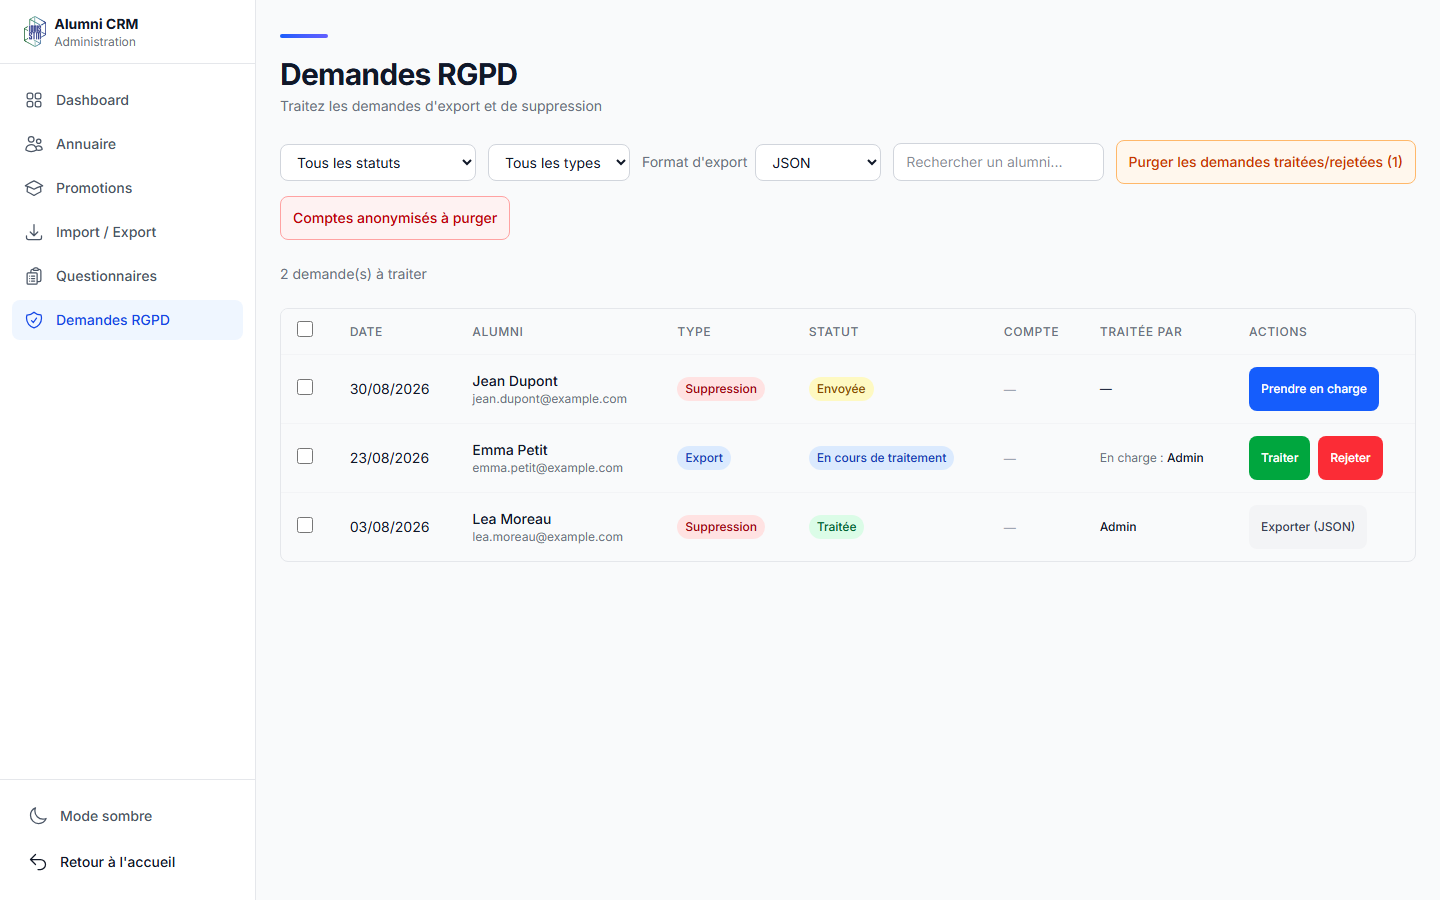
\includegraphics[width=\textwidth]{anB_demandes_rgpd_light.png}
    \caption{Mode clair.}
  \end{minipage}\hfill
  \begin{minipage}{0.48\textwidth}
    \centering
    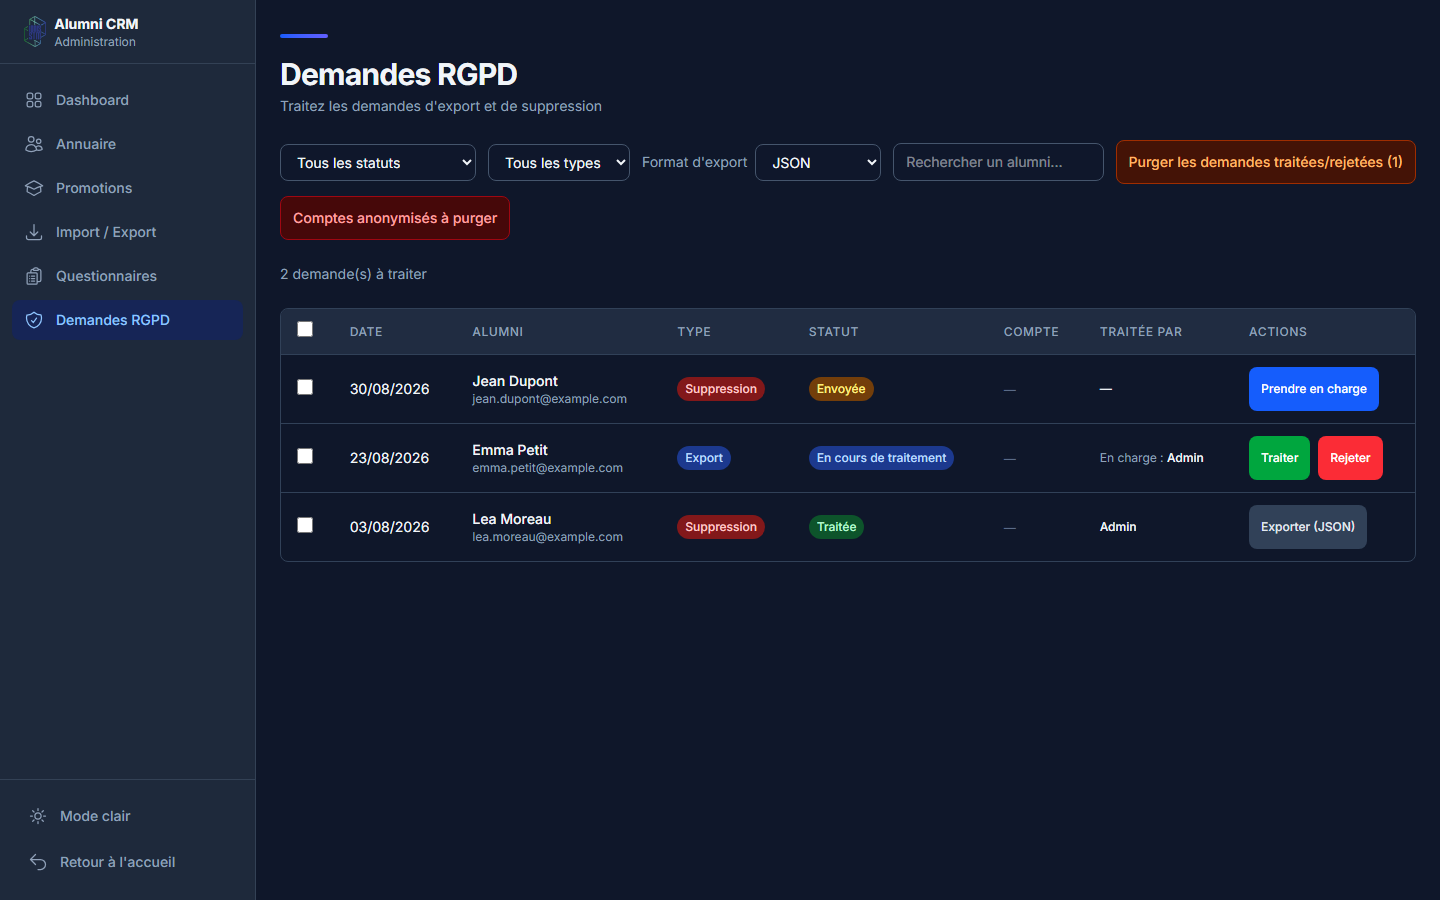
\includegraphics[width=\textwidth]{anB_demandes_rgpd_dark.png}
    \caption{Mode sombre.}
  \end{minipage}
  \caption{Gestion des demandes RGPD (workflow de traitement) -- thème clair vs thème sombre.}
\end{figure}

\begin{figure}[htbp]
  \centering
  \begin{minipage}{0.48\textwidth}
    \centering
    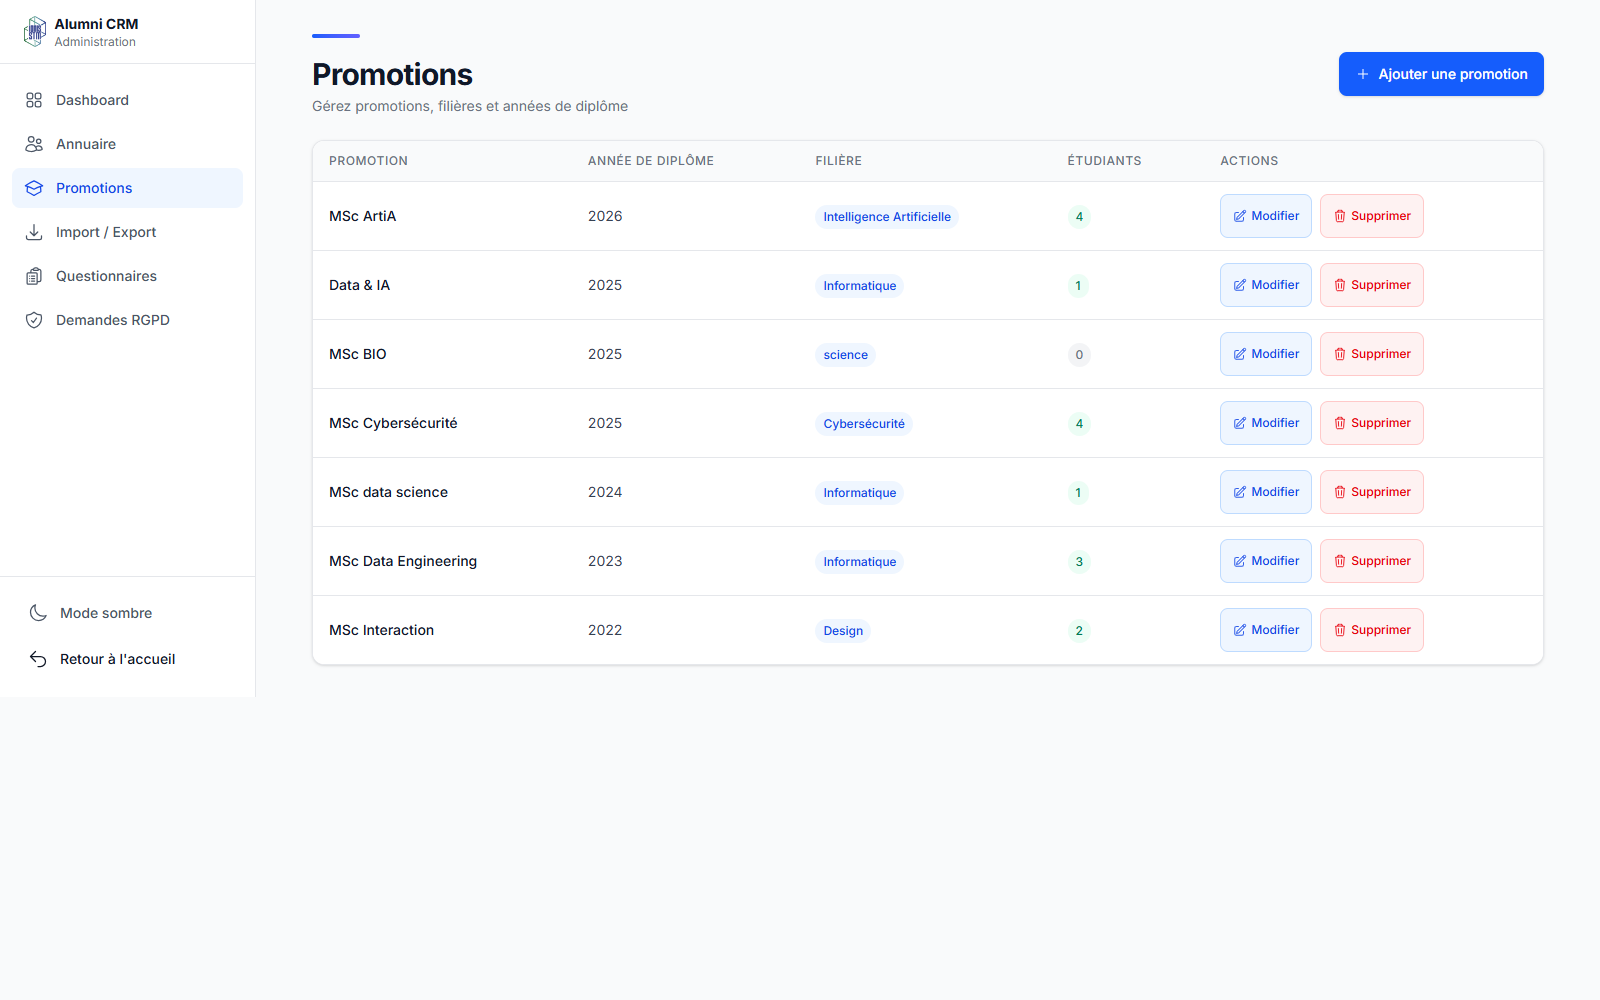
\includegraphics[width=\textwidth]{anB_promotions_light.png}
    \caption{Mode clair.}
  \end{minipage}\hfill
  \begin{minipage}{0.48\textwidth}
    \centering
    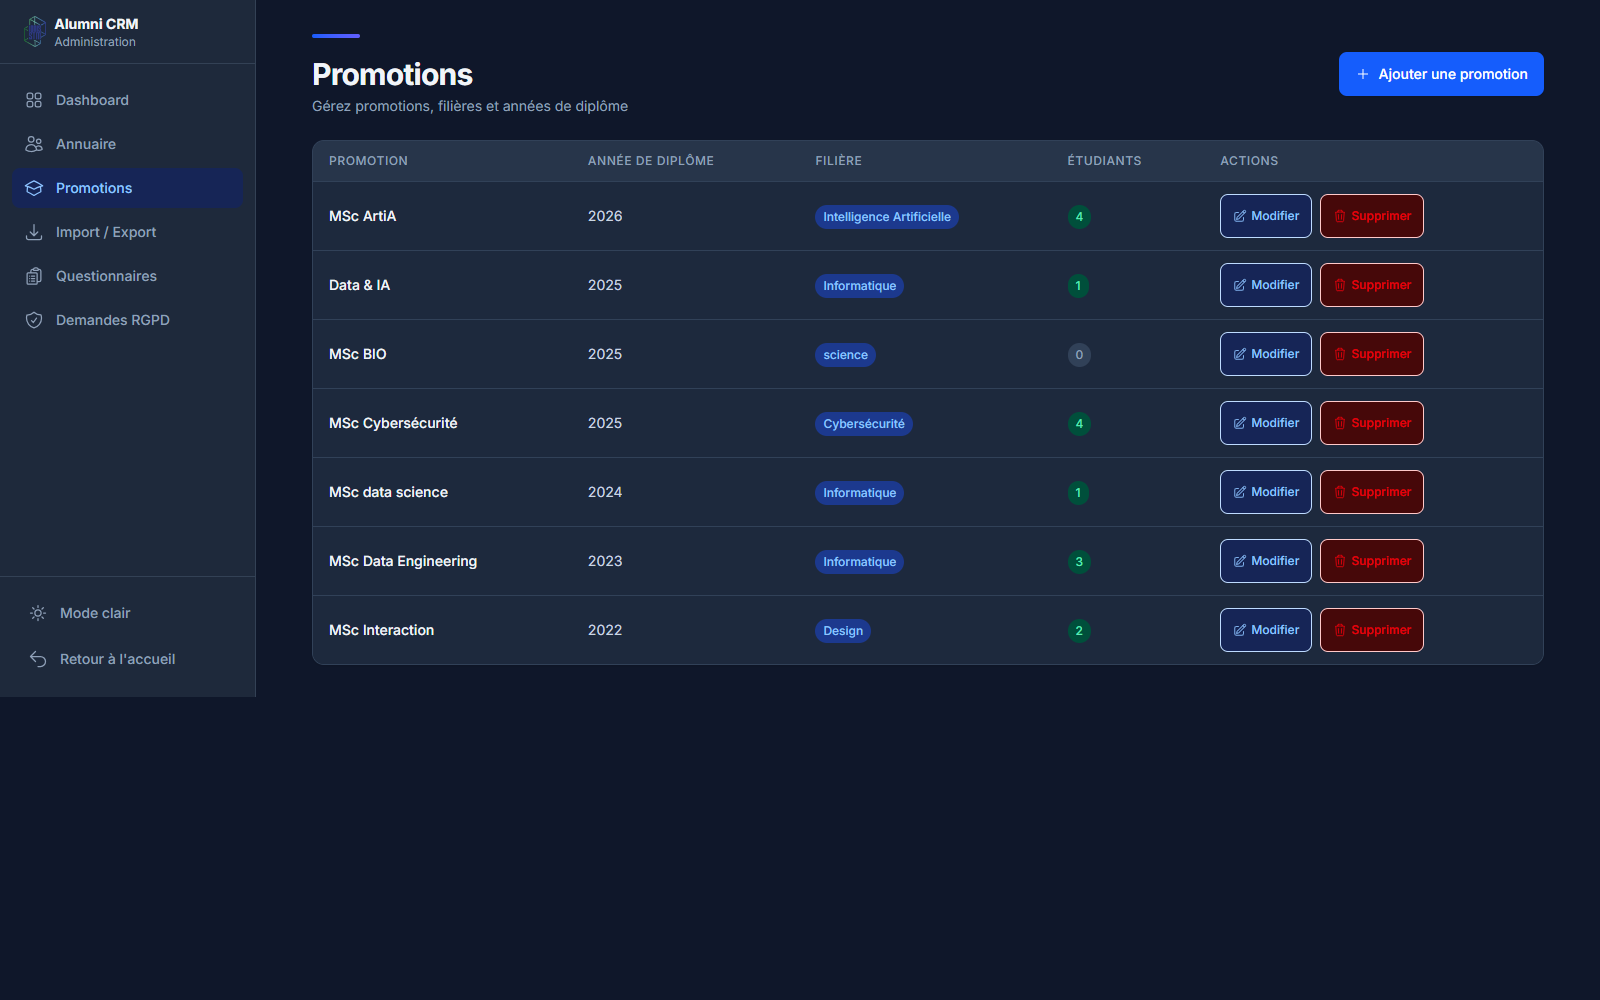
\includegraphics[width=\textwidth]{anB_promotions_dark.png}
    \caption{Mode sombre.}
  \end{minipage}
  \caption{Gestion des promotions (création, édition, suivi des effectifs) -- thème clair vs thème sombre.}
\end{figure}

\begin{figure}[htbp]
  \centering
  \begin{minipage}{0.48\textwidth}
    \centering
    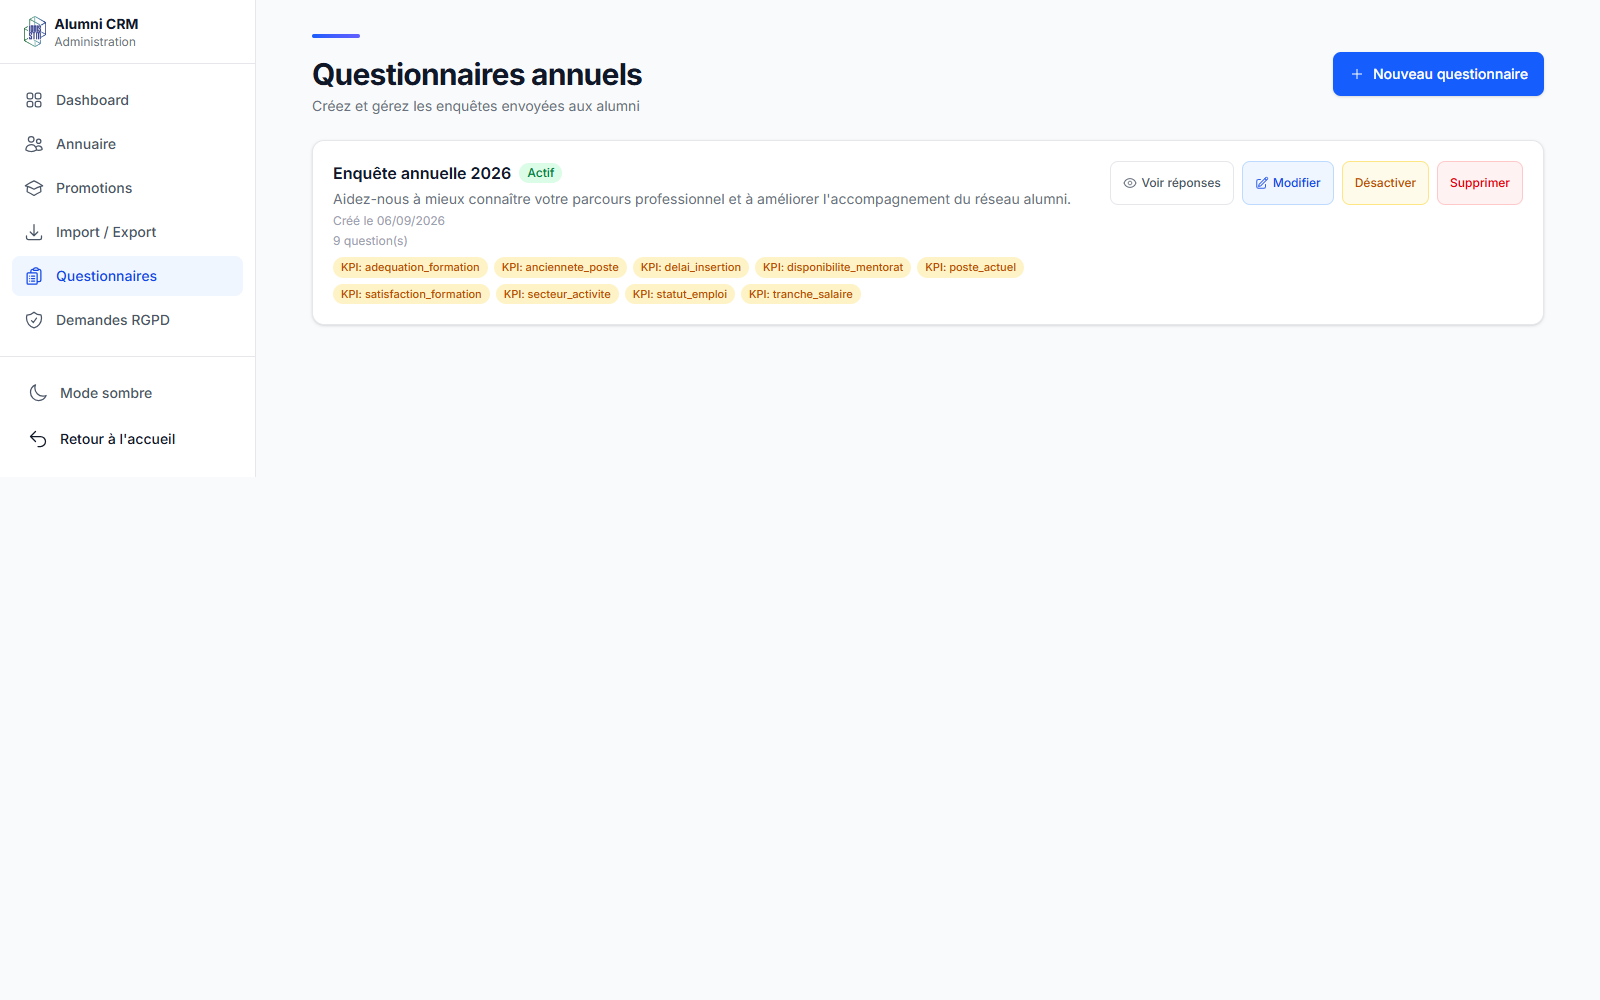
\includegraphics[width=\textwidth]{anB_questionnaires_light.png}
    \caption{Mode clair.}
  \end{minipage}\hfill
  \begin{minipage}{0.48\textwidth}
    \centering
    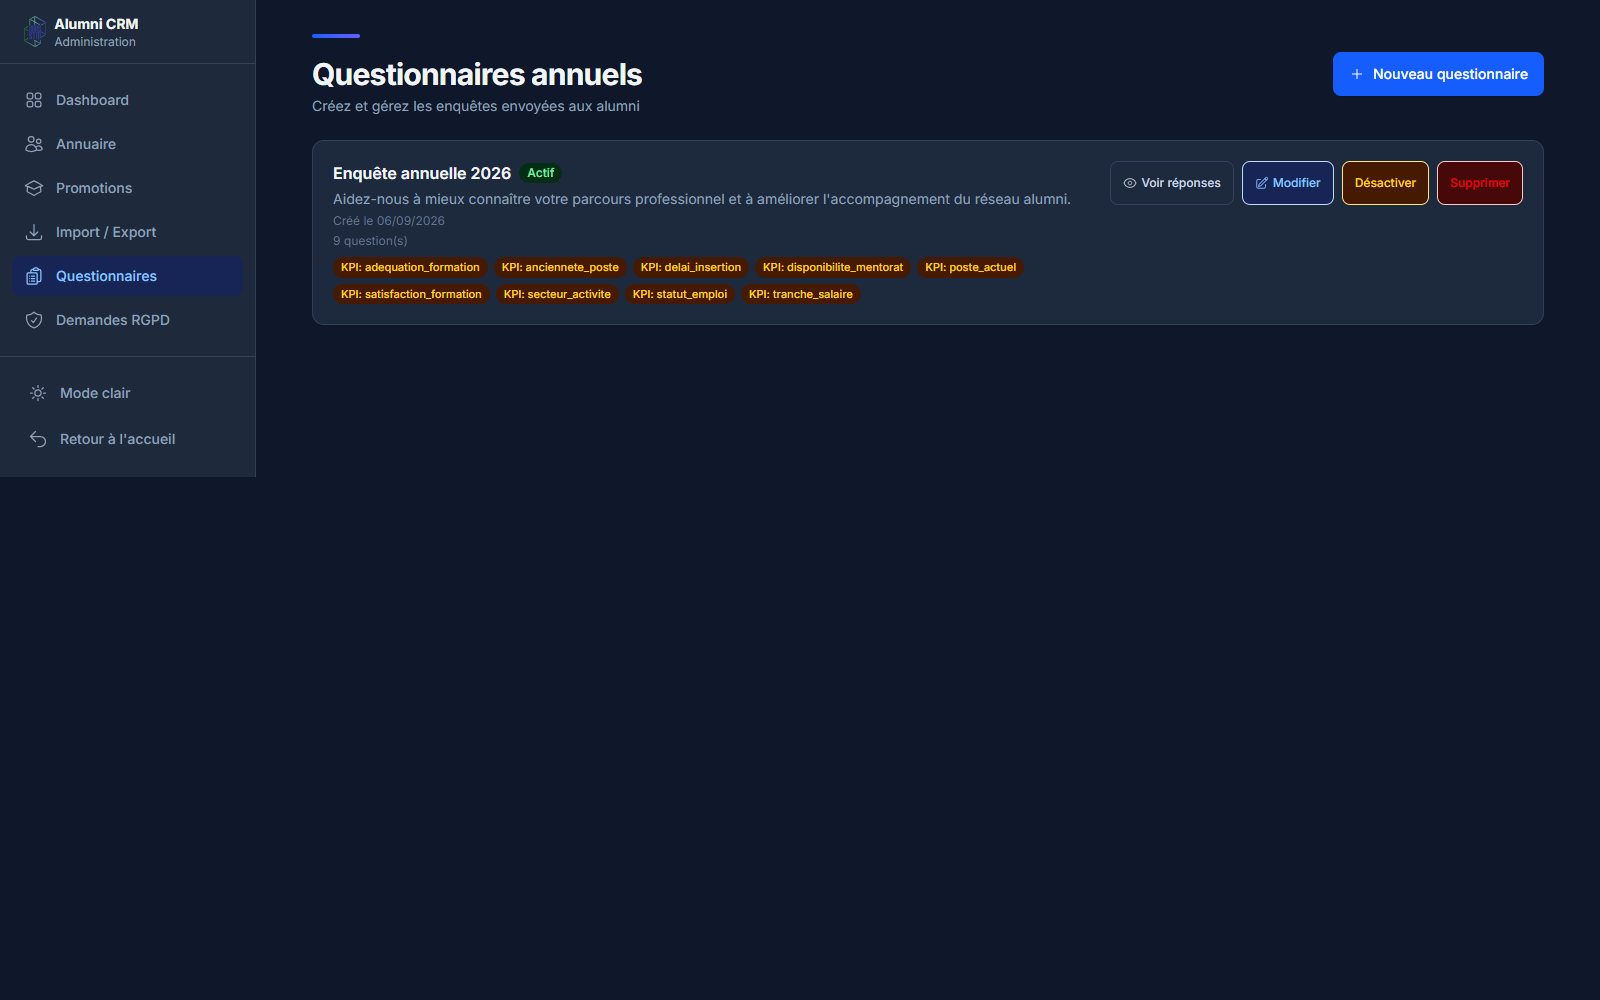
\includegraphics[width=\textwidth]{anB_questionnaires_dark.png}
    \caption{Mode sombre.}
  \end{minipage}
  \caption{Gestion des questionnaires (6 types de questions, tags KPI, conditions) -- thème clair vs thème sombre.}
\end{figure}

\begin{figure}[htbp]
  \centering
  \begin{minipage}{0.48\textwidth}
    \centering
    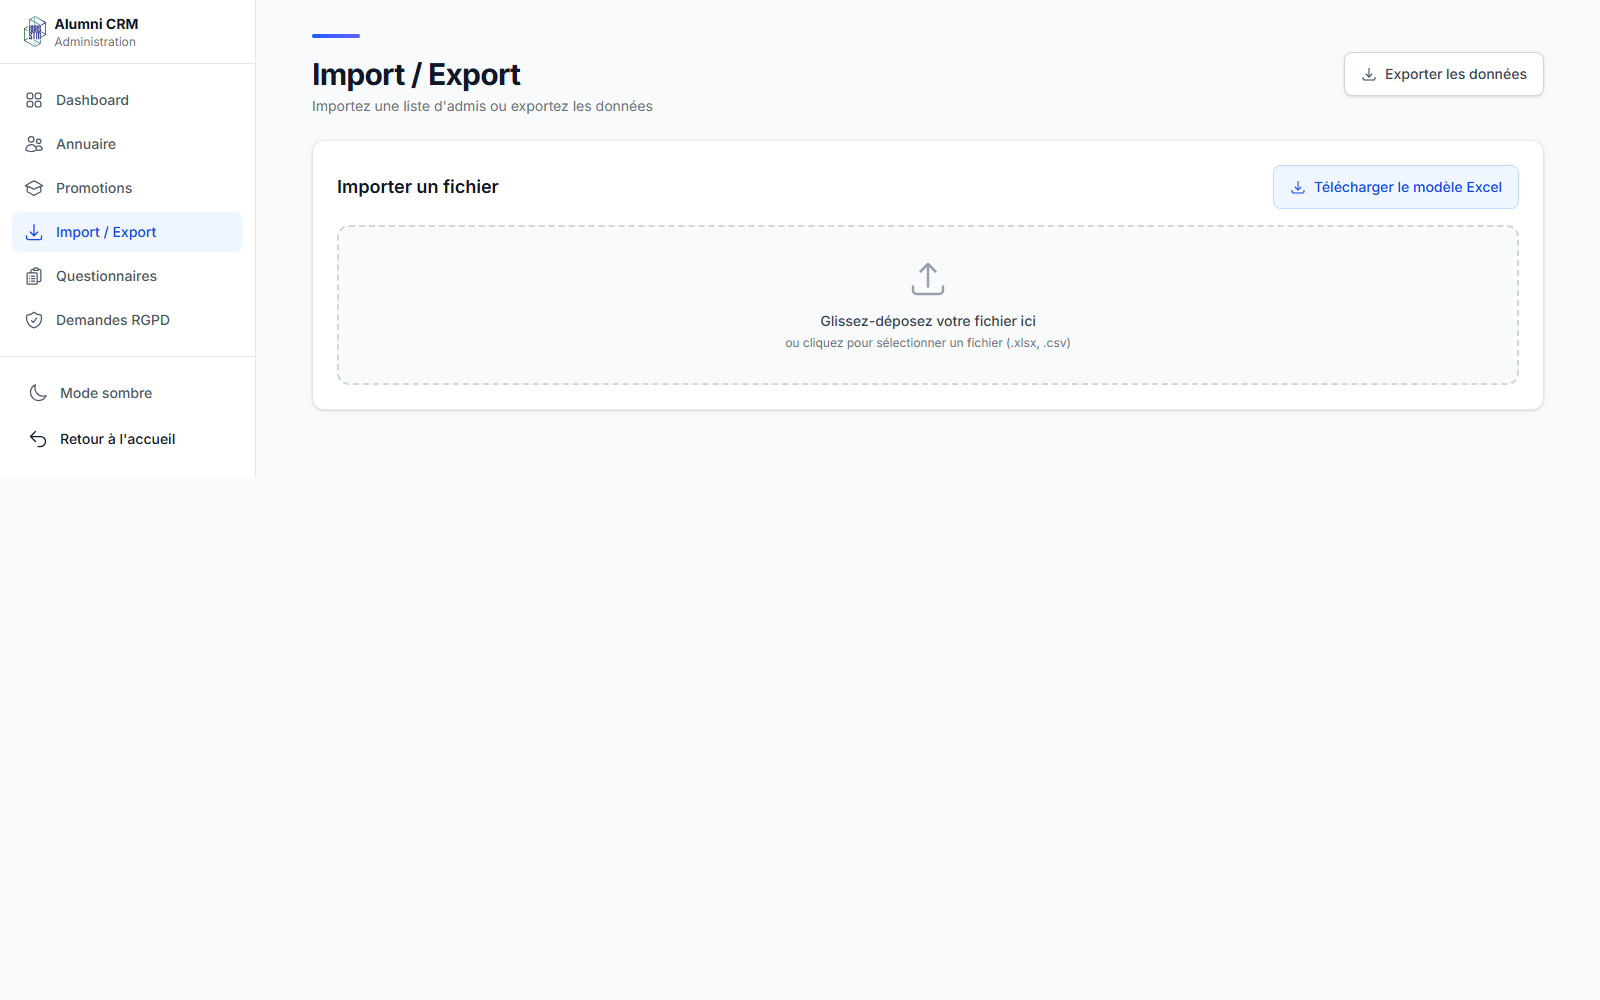
\includegraphics[width=\textwidth]{anB_import_light.png}
    \caption{Mode clair.}
  \end{minipage}\hfill
  \begin{minipage}{0.48\textwidth}
    \centering
    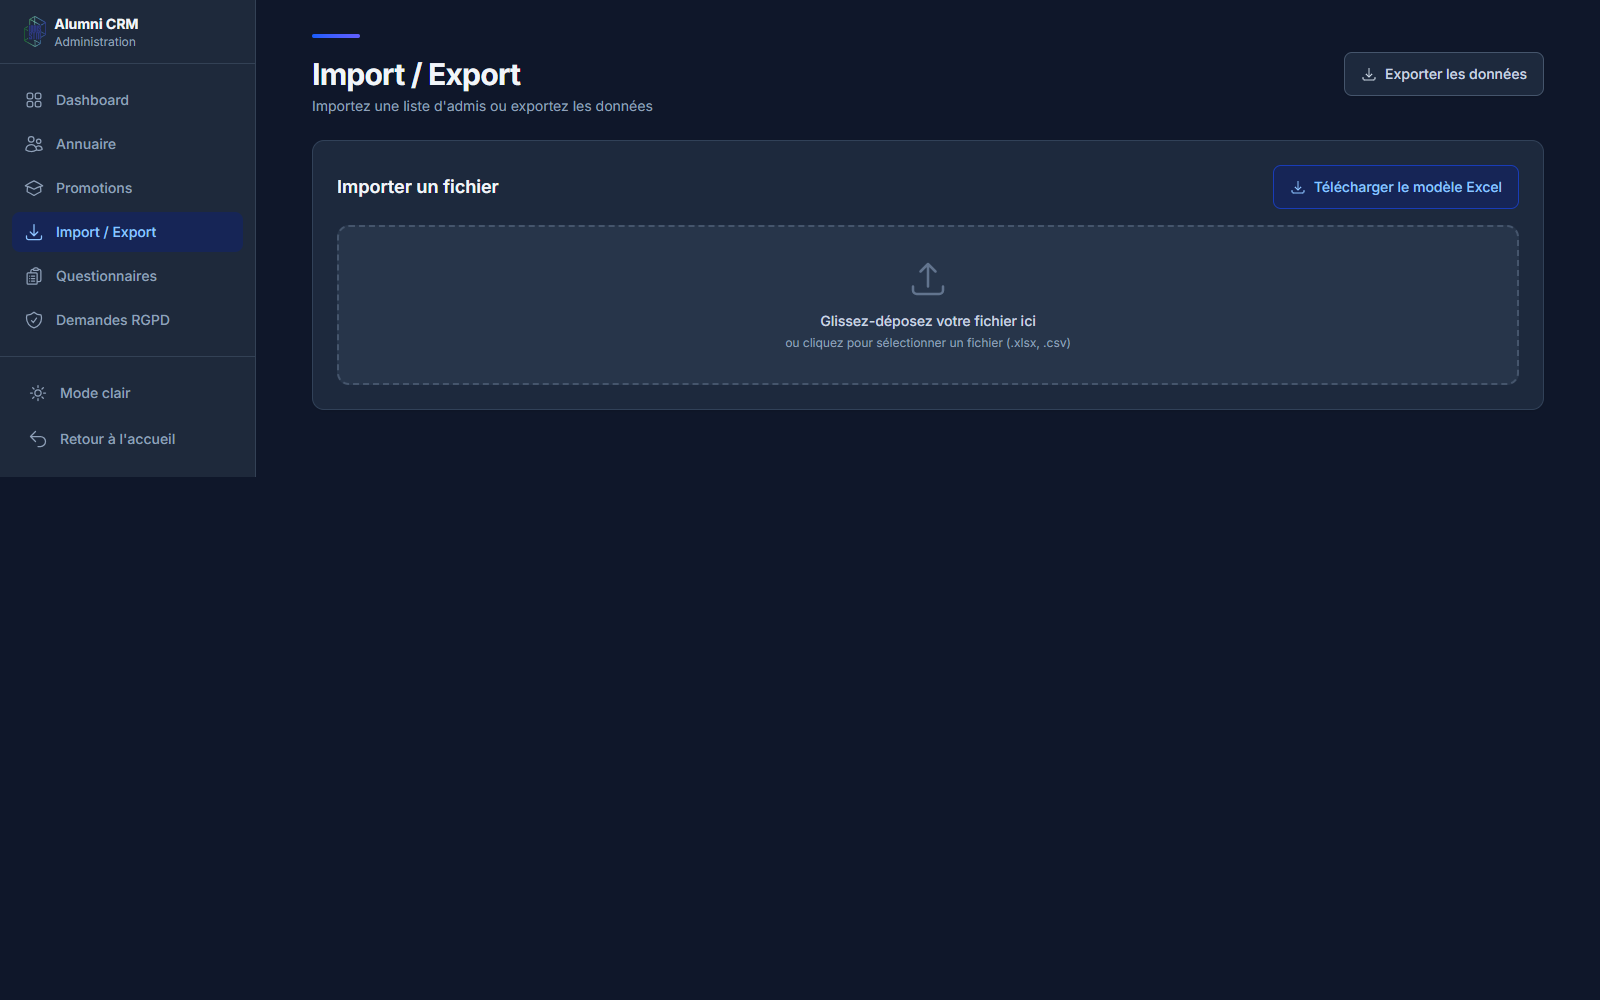
\includegraphics[width=\textwidth]{anB_import_dark.png}
    \caption{Mode sombre.}
  \end{minipage}
  \caption{Import Excel des alumni (template, rapport d'erreurs) -- thème clair vs thème sombre.}
\end{figure}

\chapter{Espace alumni (captures d'écran)}

Les captures d'écran présentent l'espace alumni~: inscription multi-étapes, profil, parcours professionnel, consentement \hyperlink{abbr-RGPD}{RGPD~(40)} et questionnaire annuel. Chaque écran est présenté en mode clair et mode sombre.

\begin{figure}[htbp]
  \centering
  \begin{minipage}{0.48\textwidth}
    \centering
    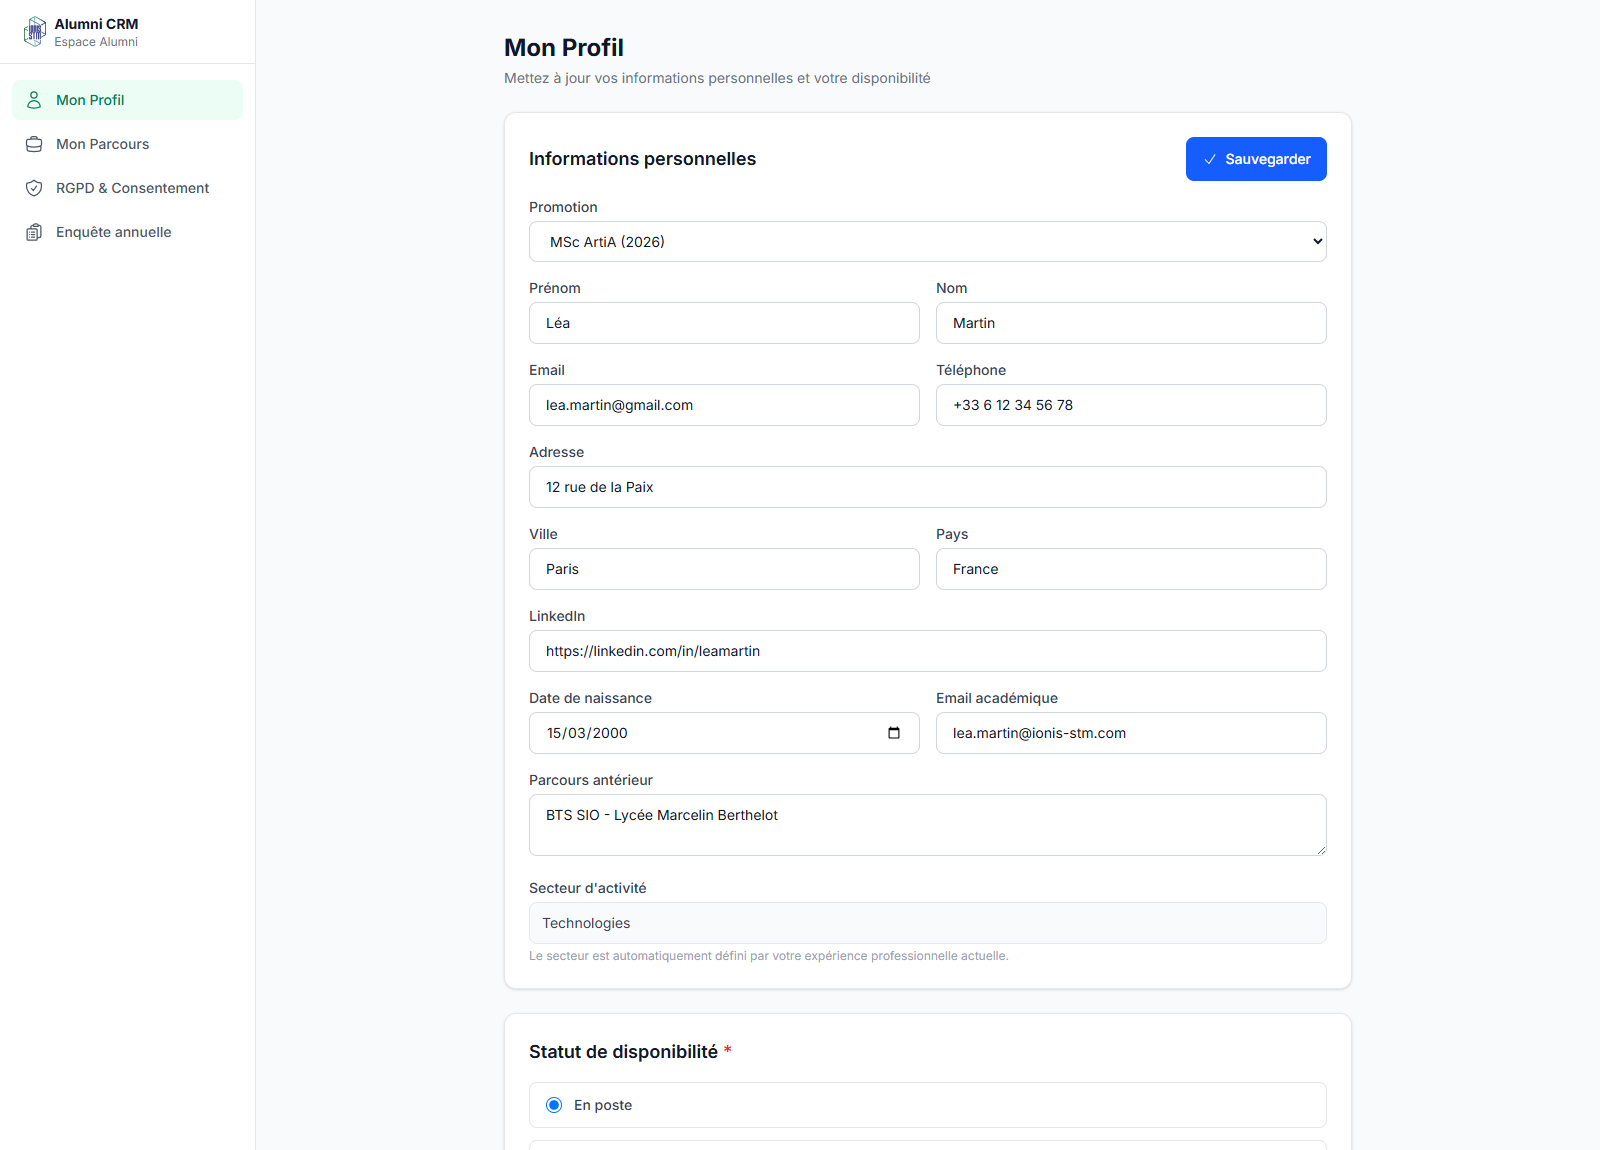
\includegraphics[width=\textwidth]{anC_profil_light_1.png}
    \caption{Mode clair -- partie 1/2.}
  \end{minipage}\hfill
  \begin{minipage}{0.48\textwidth}
    \centering
    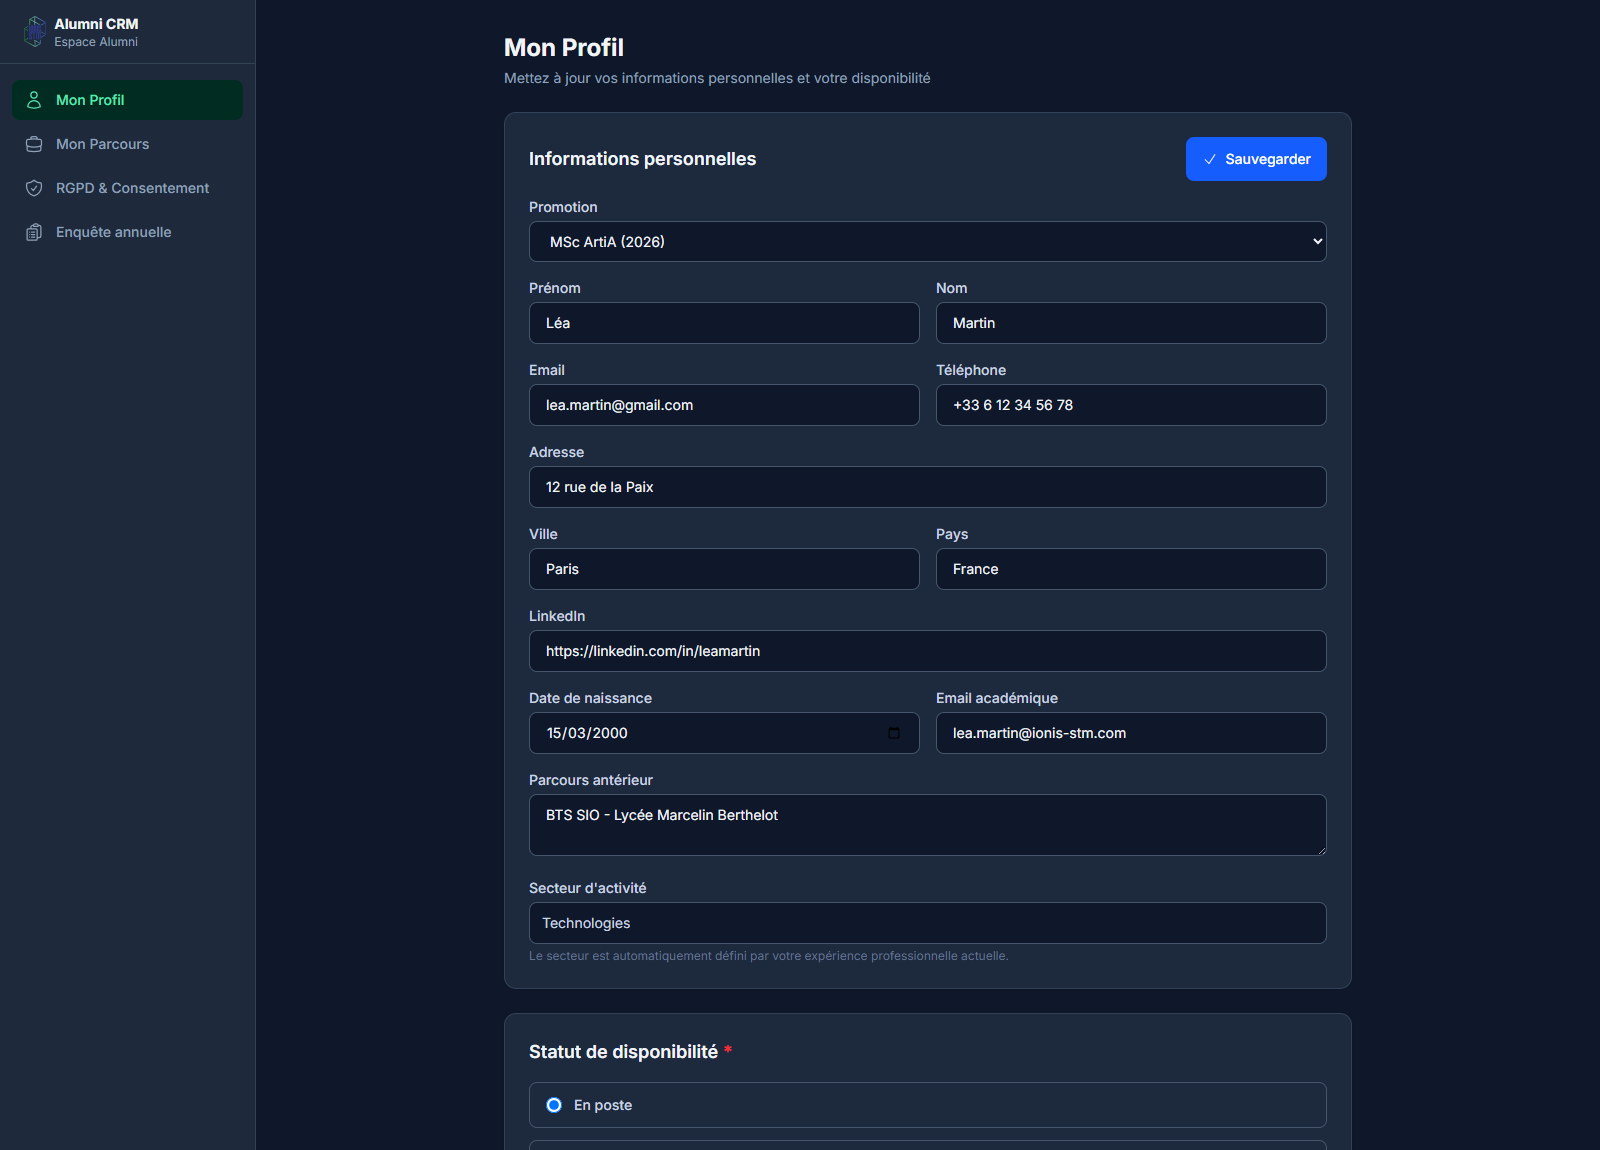
\includegraphics[width=\textwidth]{anC_profil_dark_1.png}
    \caption{Mode sombre -- partie 1/2.}
  \end{minipage}

  \medskip

  \begin{minipage}{0.48\textwidth}
    \centering
    
\includegraphics[width=\textwidth]{anC_profil_light_2.png}
    \caption{Mode clair -- partie 2/2.}
  \end{minipage}\hfill
  \begin{minipage}{0.48\textwidth}
    \centering
    
\includegraphics[width=\textwidth]{anC_profil_dark_2.png}
    \caption{Mode sombre -- partie 2/2.}
  \end{minipage}
  \caption{Profil alumni (identité, statut de disponibilité, promotion, compétences) -- thème clair vs thème sombre, capture intégrale en deux parties.}
\end{figure}

\begin{figure}[htbp]
  \centering
  \begin{minipage}{0.48\textwidth}
    \centering
    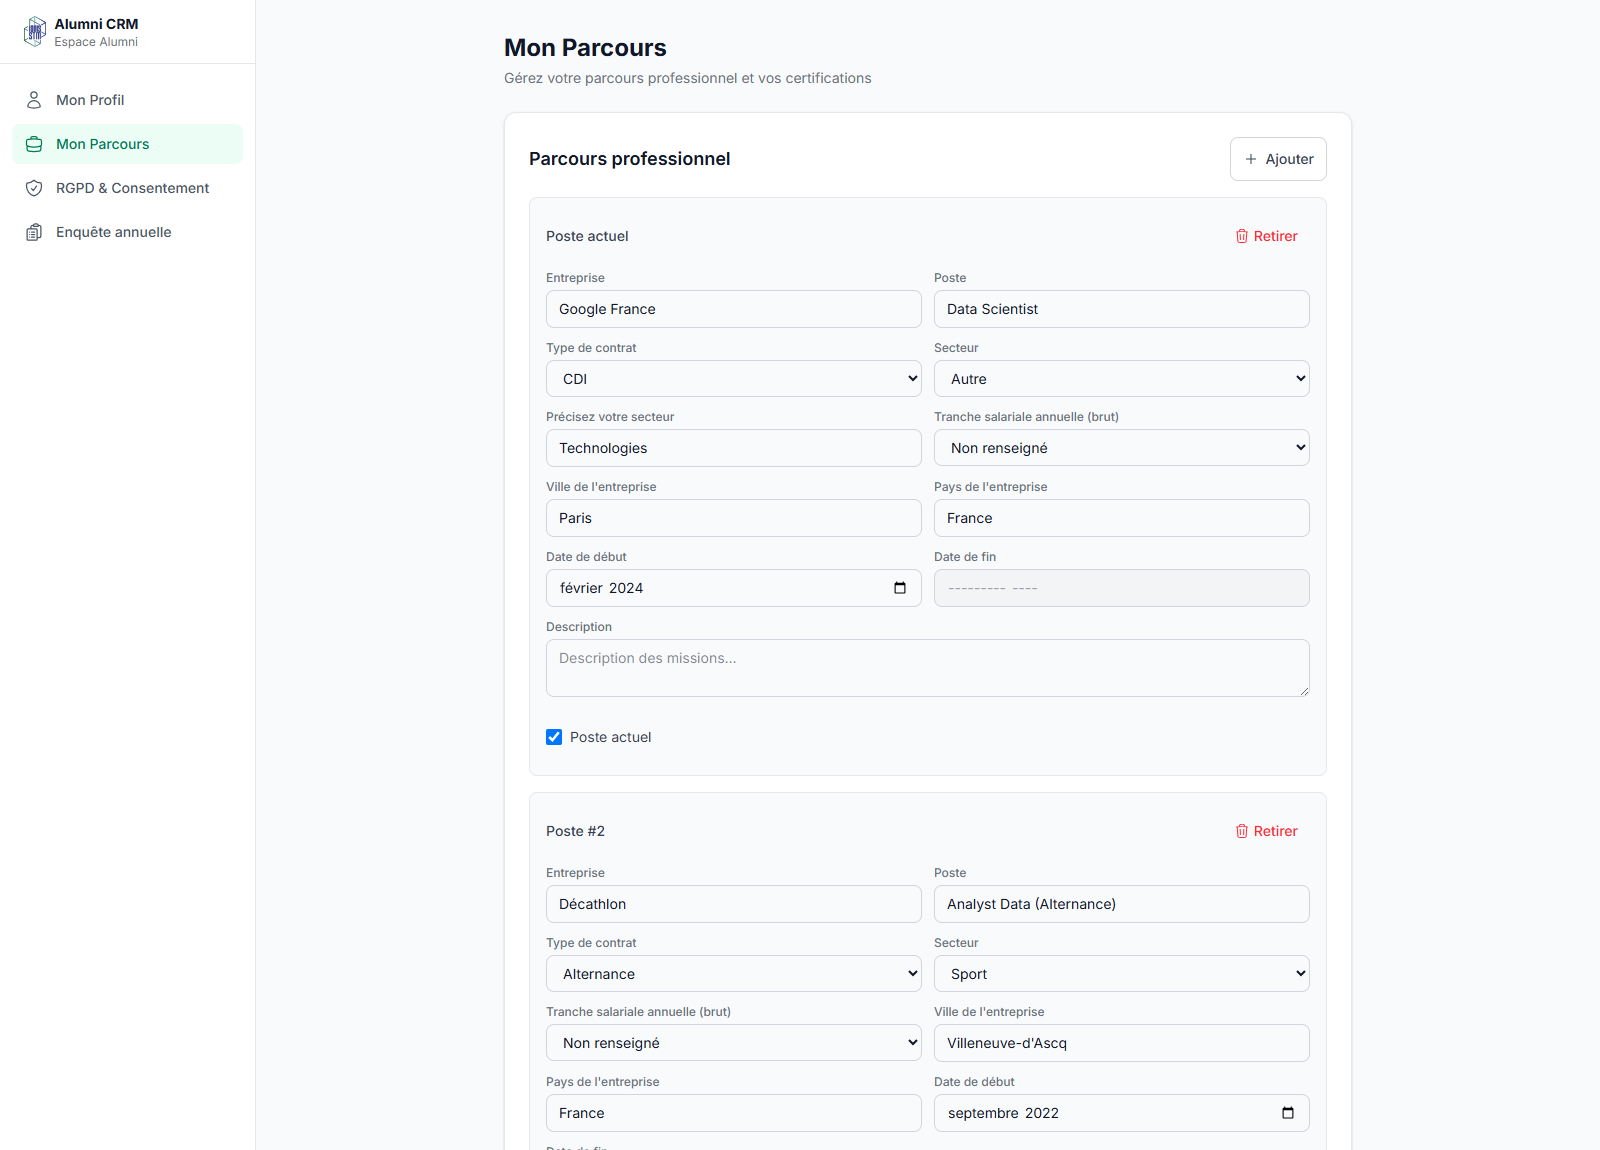
\includegraphics[width=\textwidth]{anC_parcours_light_1.png}
    \caption{Mode clair -- partie 1/2.}
  \end{minipage}\hfill
  \begin{minipage}{0.48\textwidth}
    \centering
    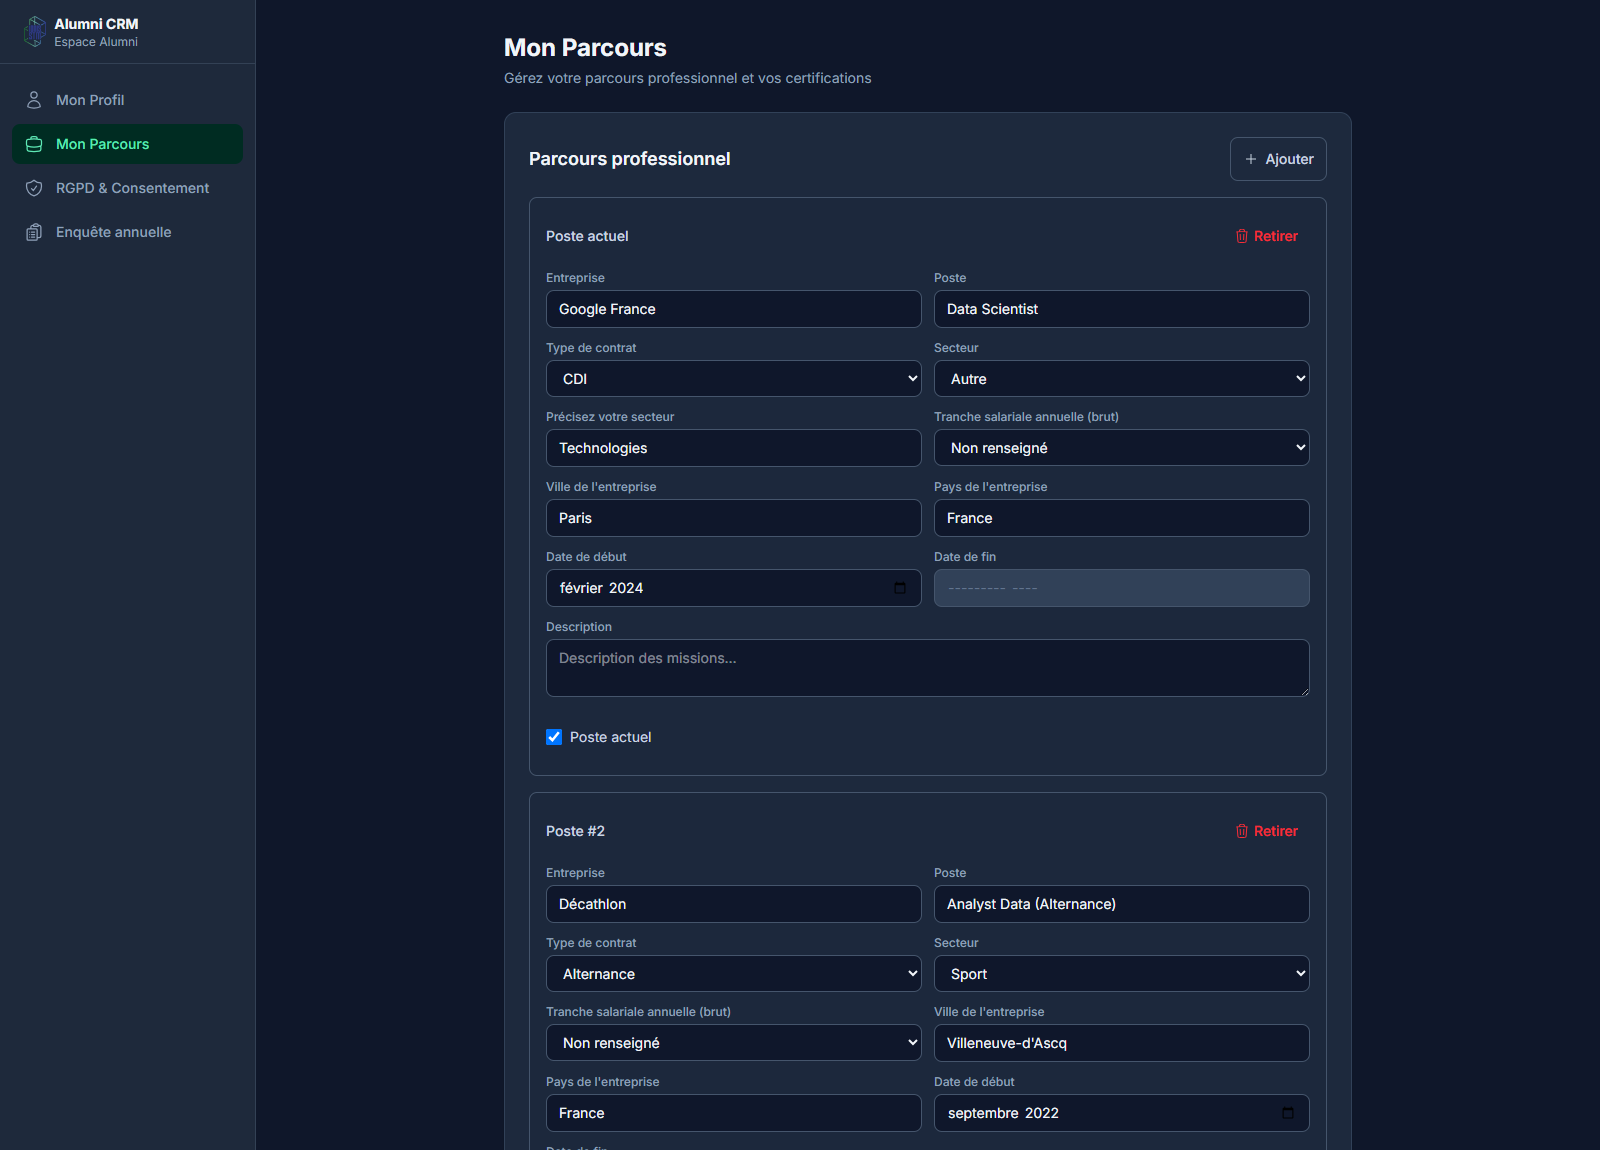
\includegraphics[width=\textwidth]{anC_parcours_dark_1.png}
    \caption{Mode sombre -- partie 1/2.}
  \end{minipage}

  \medskip

  \begin{minipage}{0.48\textwidth}
    \centering
    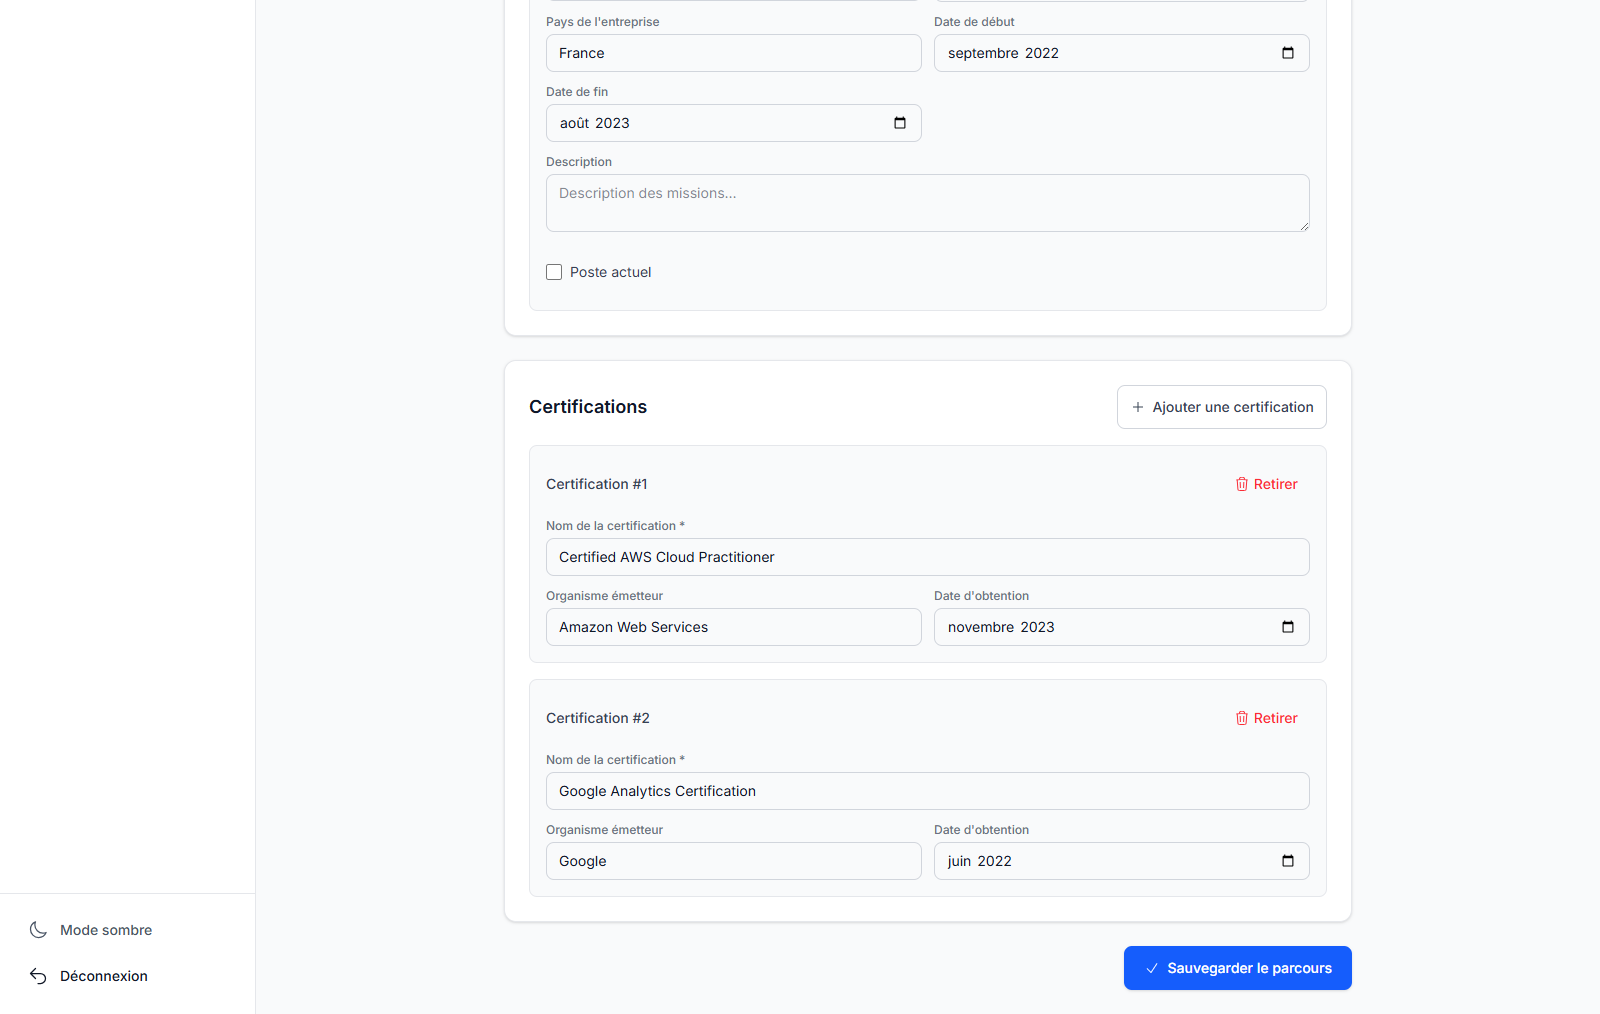
\includegraphics[width=\textwidth]{anC_parcours_light_2.png}
    \caption{Mode clair -- partie 2/2.}
  \end{minipage}\hfill
  \begin{minipage}{0.48\textwidth}
    \centering
    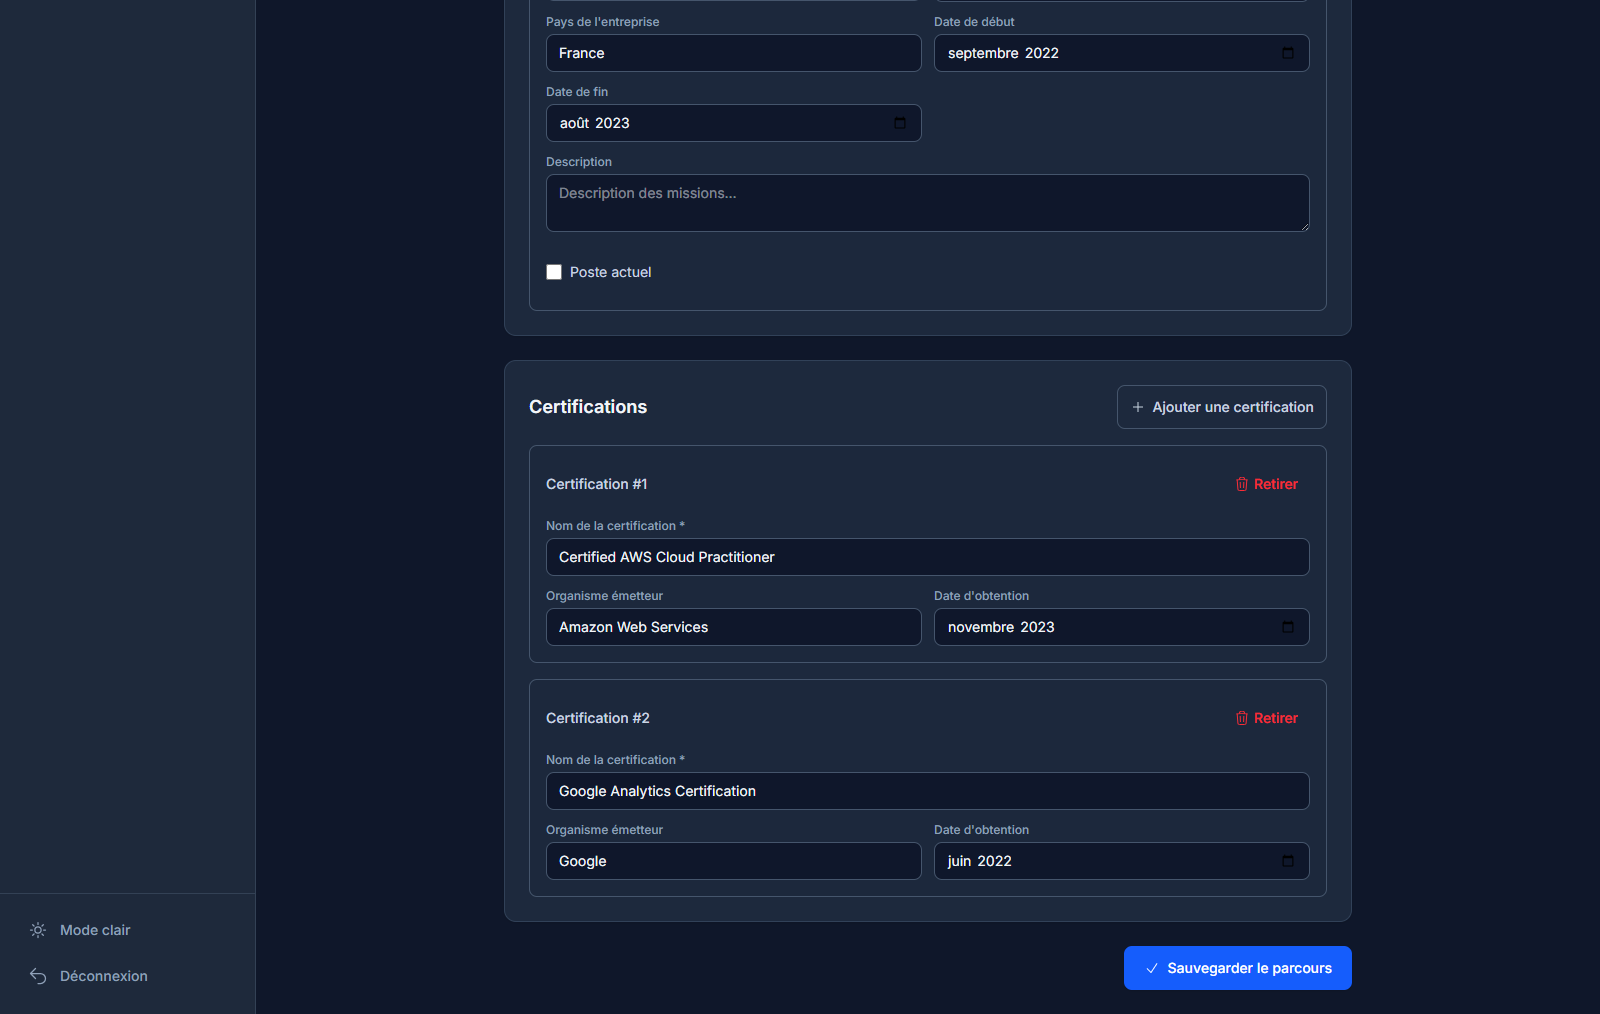
\includegraphics[width=\textwidth]{anC_parcours_dark_2.png}
    \caption{Mode sombre -- partie 2/2.}
  \end{minipage}
  \caption{Parcours professionnel (expériences et certifications) -- thème clair vs thème sombre, capture intégrale en deux parties.}
\end{figure}

\begin{figure}[htbp]
  \centering
  \begin{minipage}{0.48\textwidth}
    \centering
    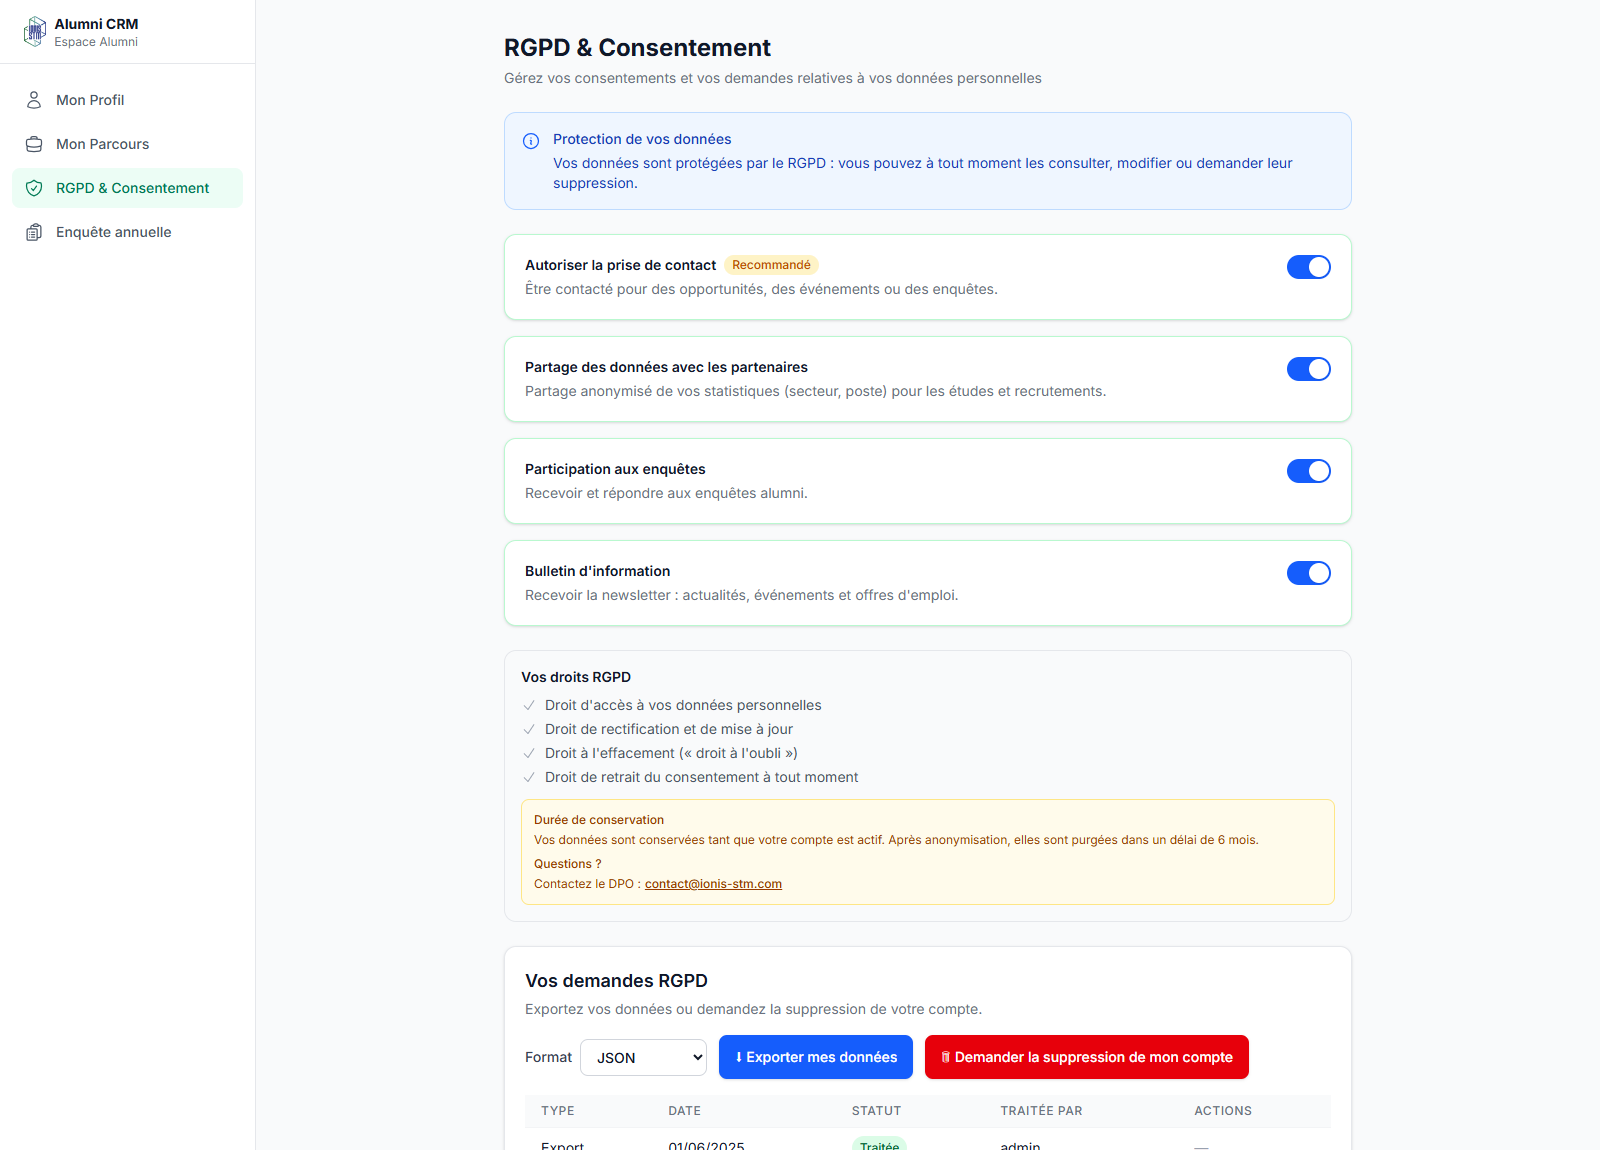
\includegraphics[width=\textwidth]{anC_consentement_light_1.png}
    \caption{Mode clair -- partie 1/2.}
  \end{minipage}\hfill
  \begin{minipage}{0.48\textwidth}
    \centering
    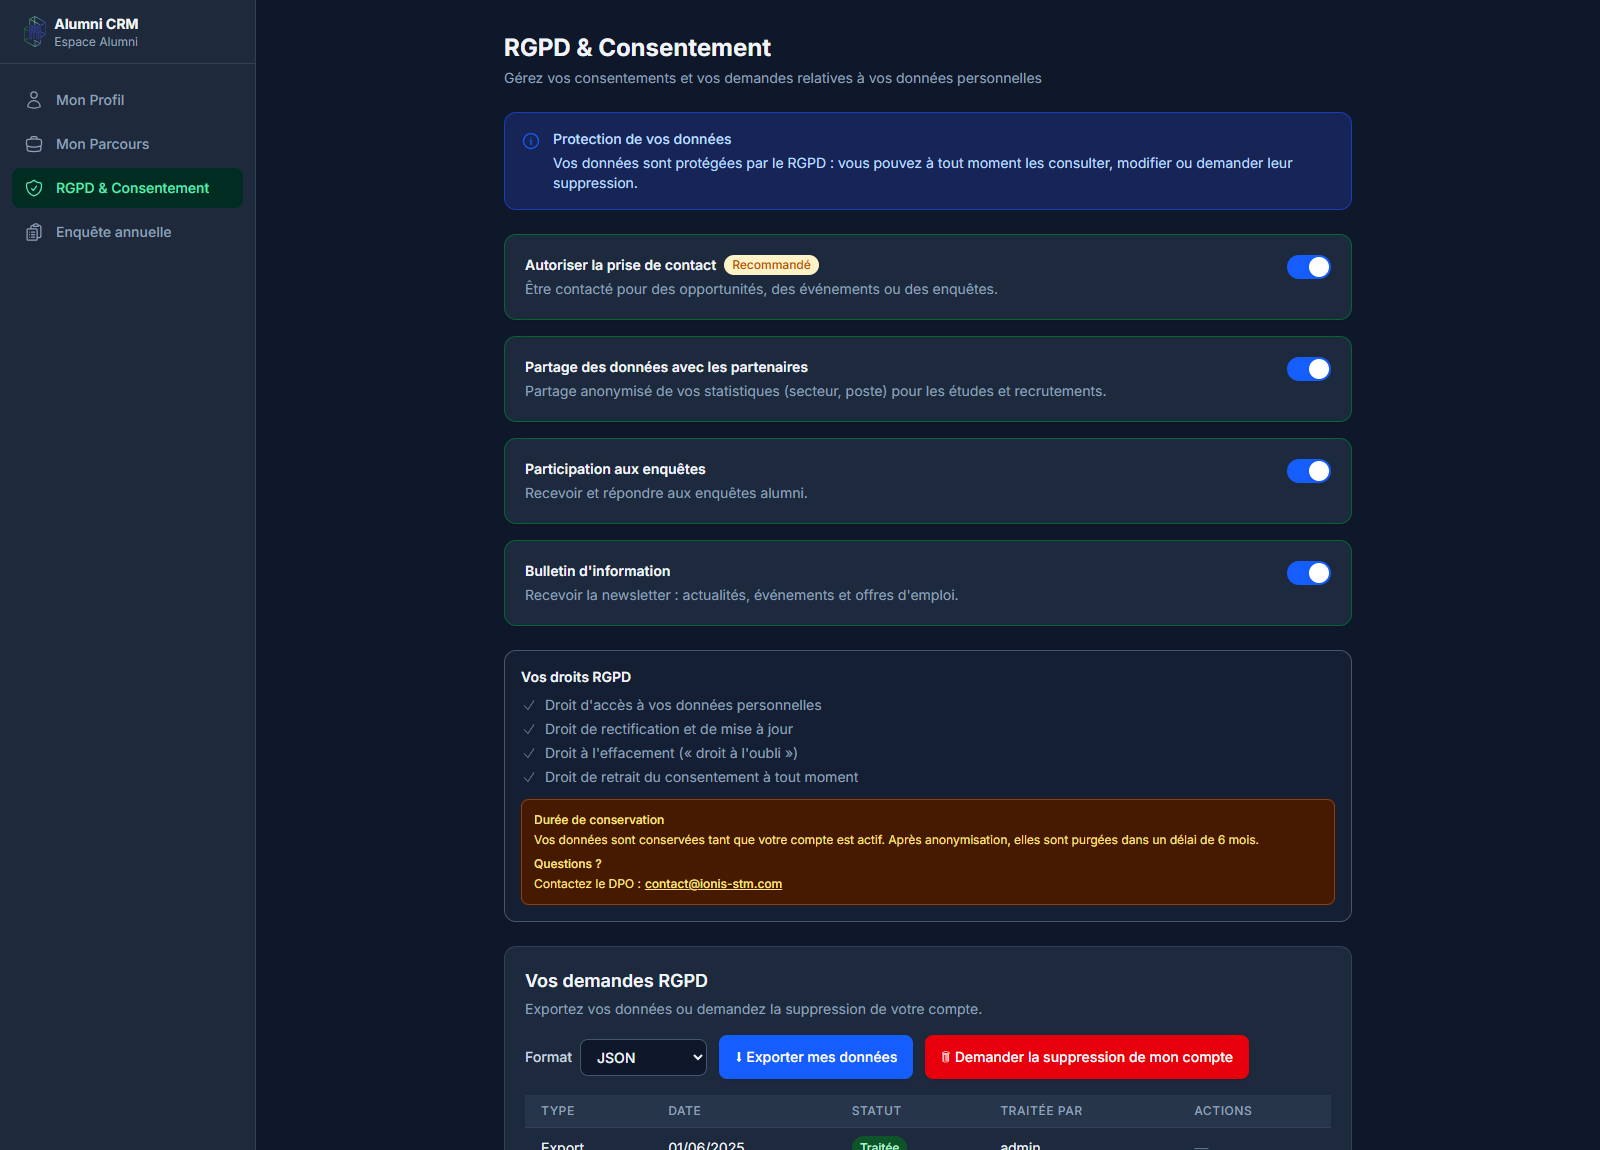
\includegraphics[width=\textwidth]{anC_consentement_dark_1.png}
    \caption{Mode sombre -- partie 1/2.}
  \end{minipage}

  \medskip

  \begin{minipage}{0.48\textwidth}
    \centering
    
\includegraphics[width=\textwidth]{anC_consentement_light_2.png}
    \caption{Mode clair -- partie 2/2.}
  \end{minipage}\hfill
  \begin{minipage}{0.48\textwidth}
    \centering
    
\includegraphics[width=\textwidth]{anC_consentement_dark_2.png}
    \caption{Mode sombre -- partie 2/2.}
  \end{minipage}
  \caption{Gestion du consentement RGPD (4 types, export, demande de suppression) -- thème clair vs thème sombre, capture intégrale en deux parties.}
\end{figure}

\begin{figure}[htbp]
  \centering
  \begin{minipage}{0.48\textwidth}
    \centering
    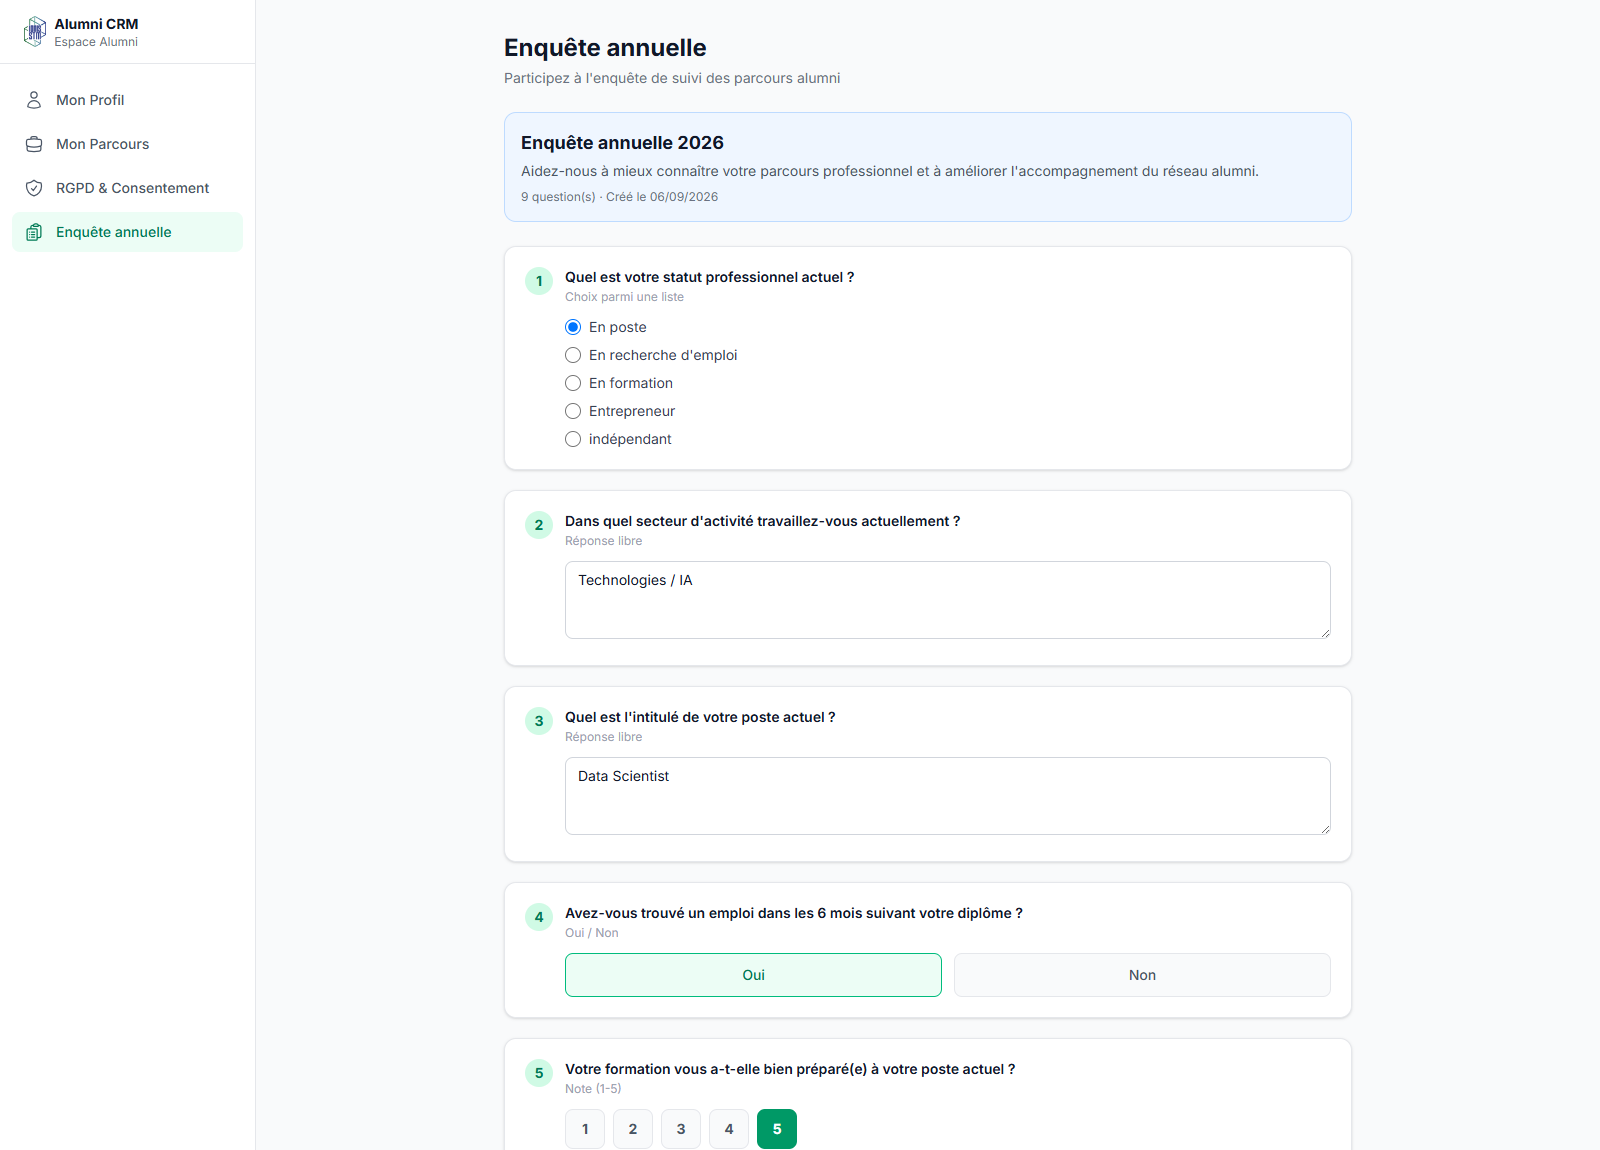
\includegraphics[width=\textwidth]{anC_questionnaire_light_1.png}
    \caption{Mode clair -- partie 1/2.}
  \end{minipage}\hfill
  \begin{minipage}{0.48\textwidth}
    \centering
    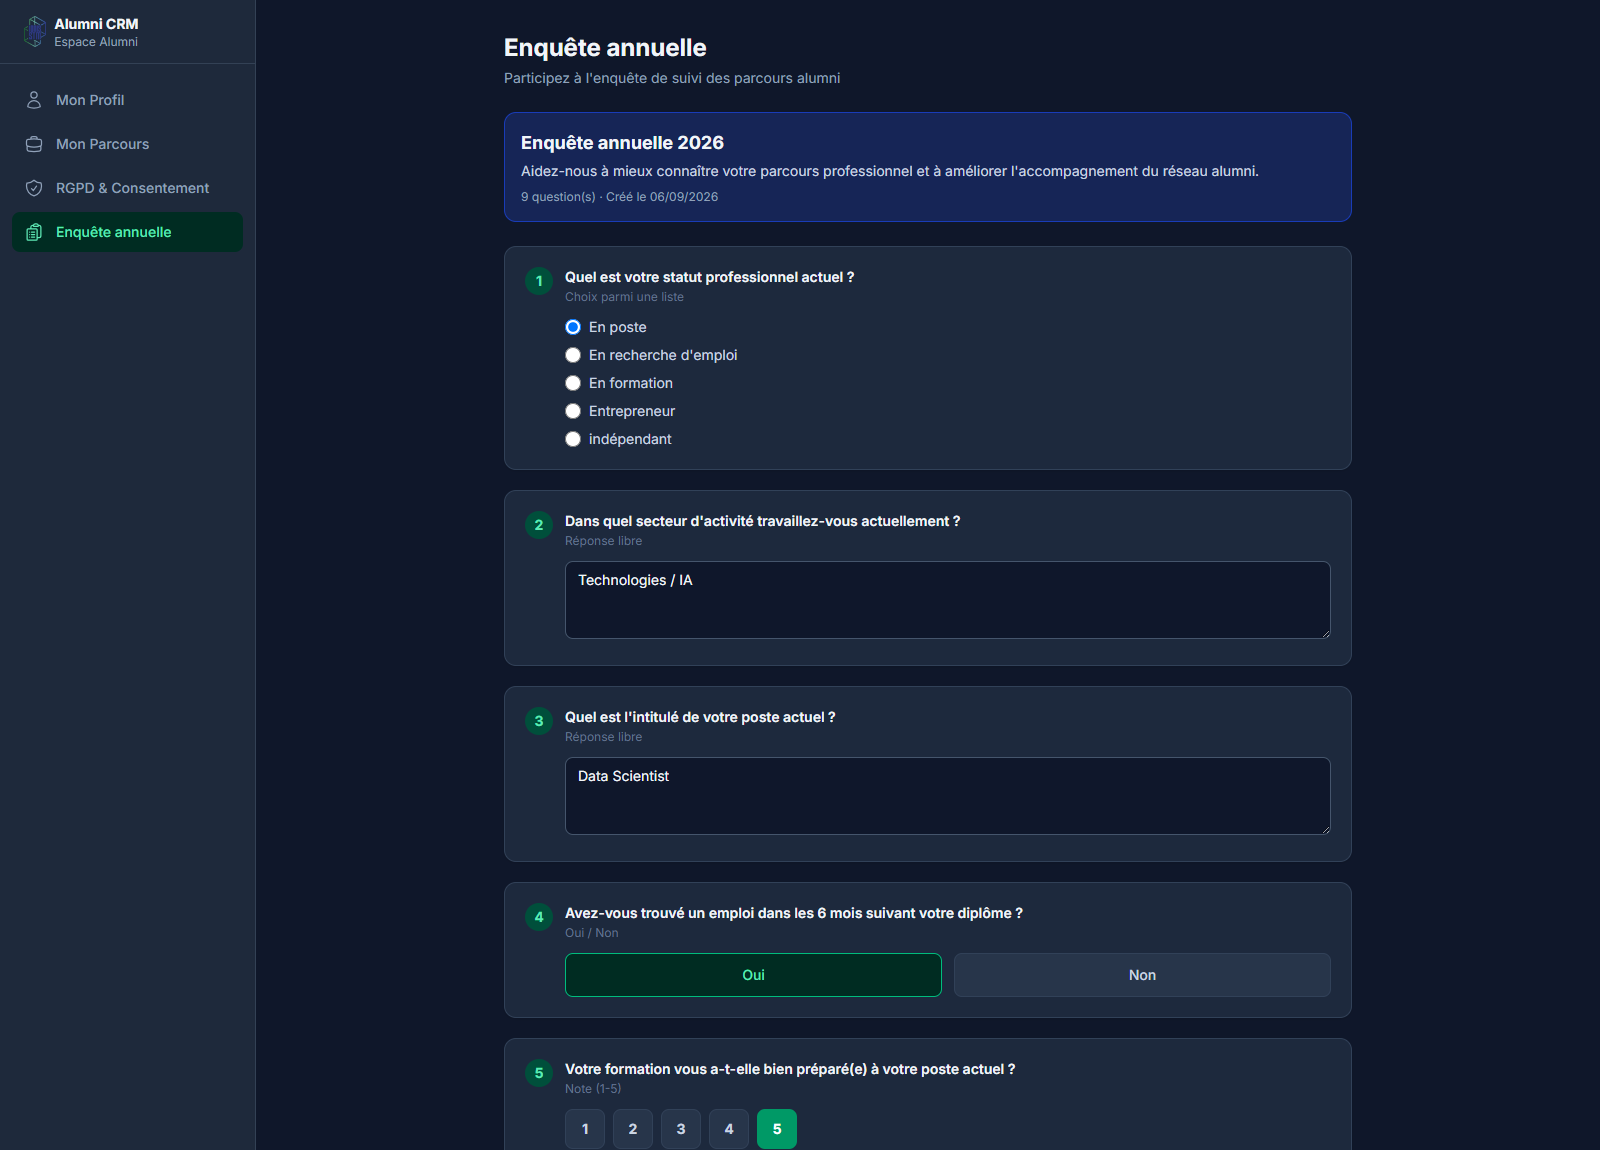
\includegraphics[width=\textwidth]{anC_questionnaire_dark_1.png}
    \caption{Mode sombre -- partie 1/2.}
  \end{minipage}

  \medskip

  \begin{minipage}{0.48\textwidth}
    \centering
    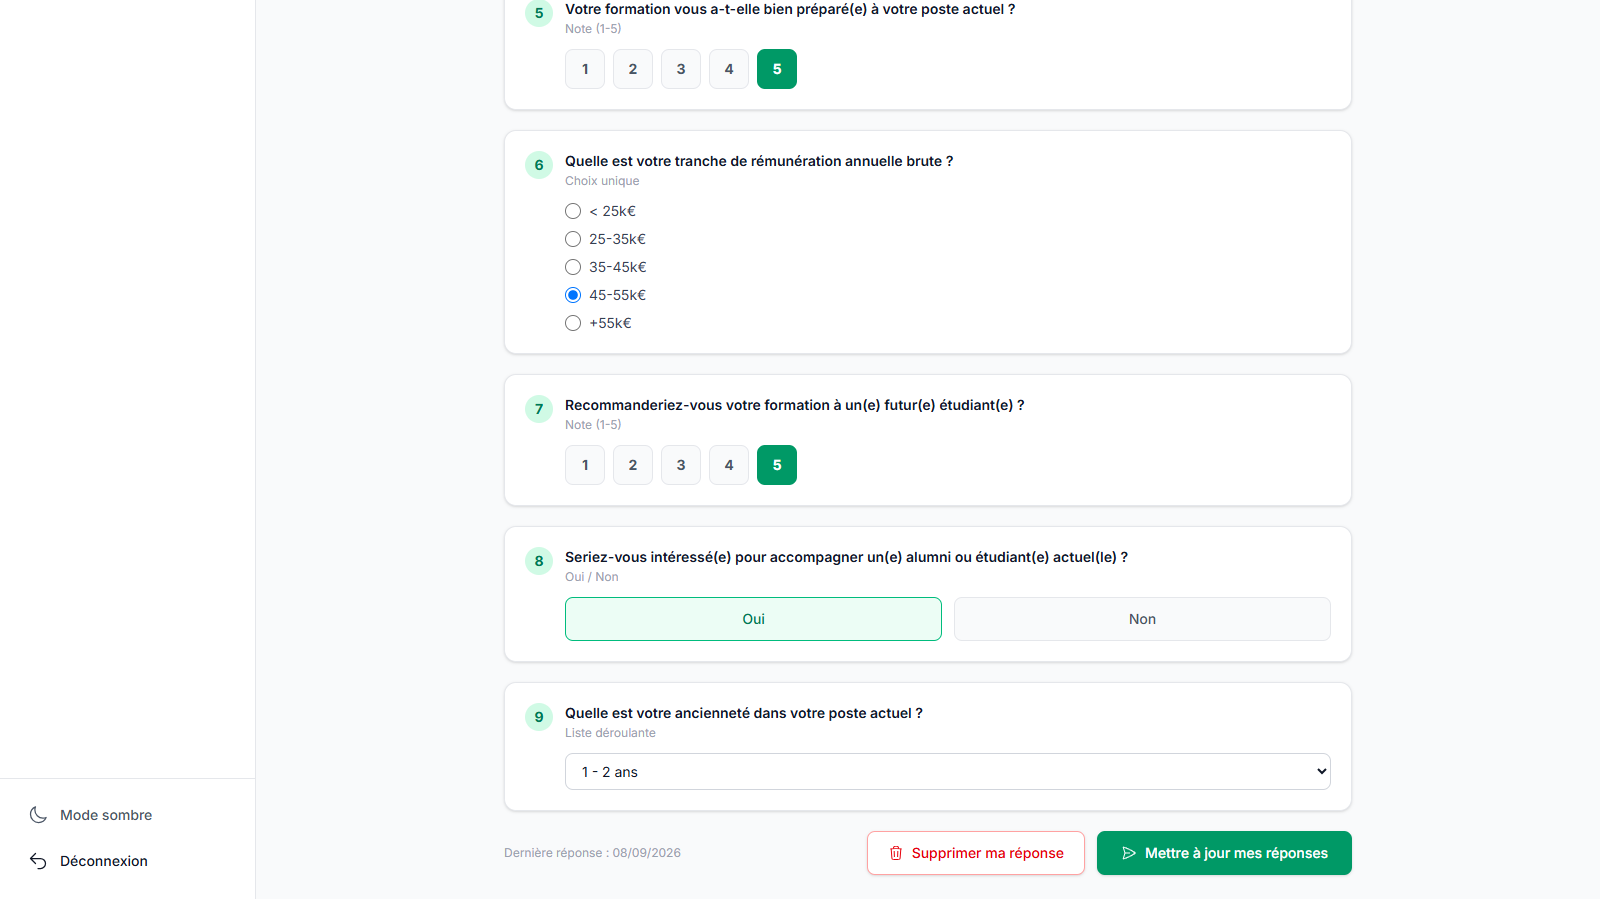
\includegraphics[width=\textwidth]{anC_questionnaire_light_2.png}
    \caption{Mode clair -- partie 2/2.}
  \end{minipage}\hfill
  \begin{minipage}{0.48\textwidth}
    \centering
    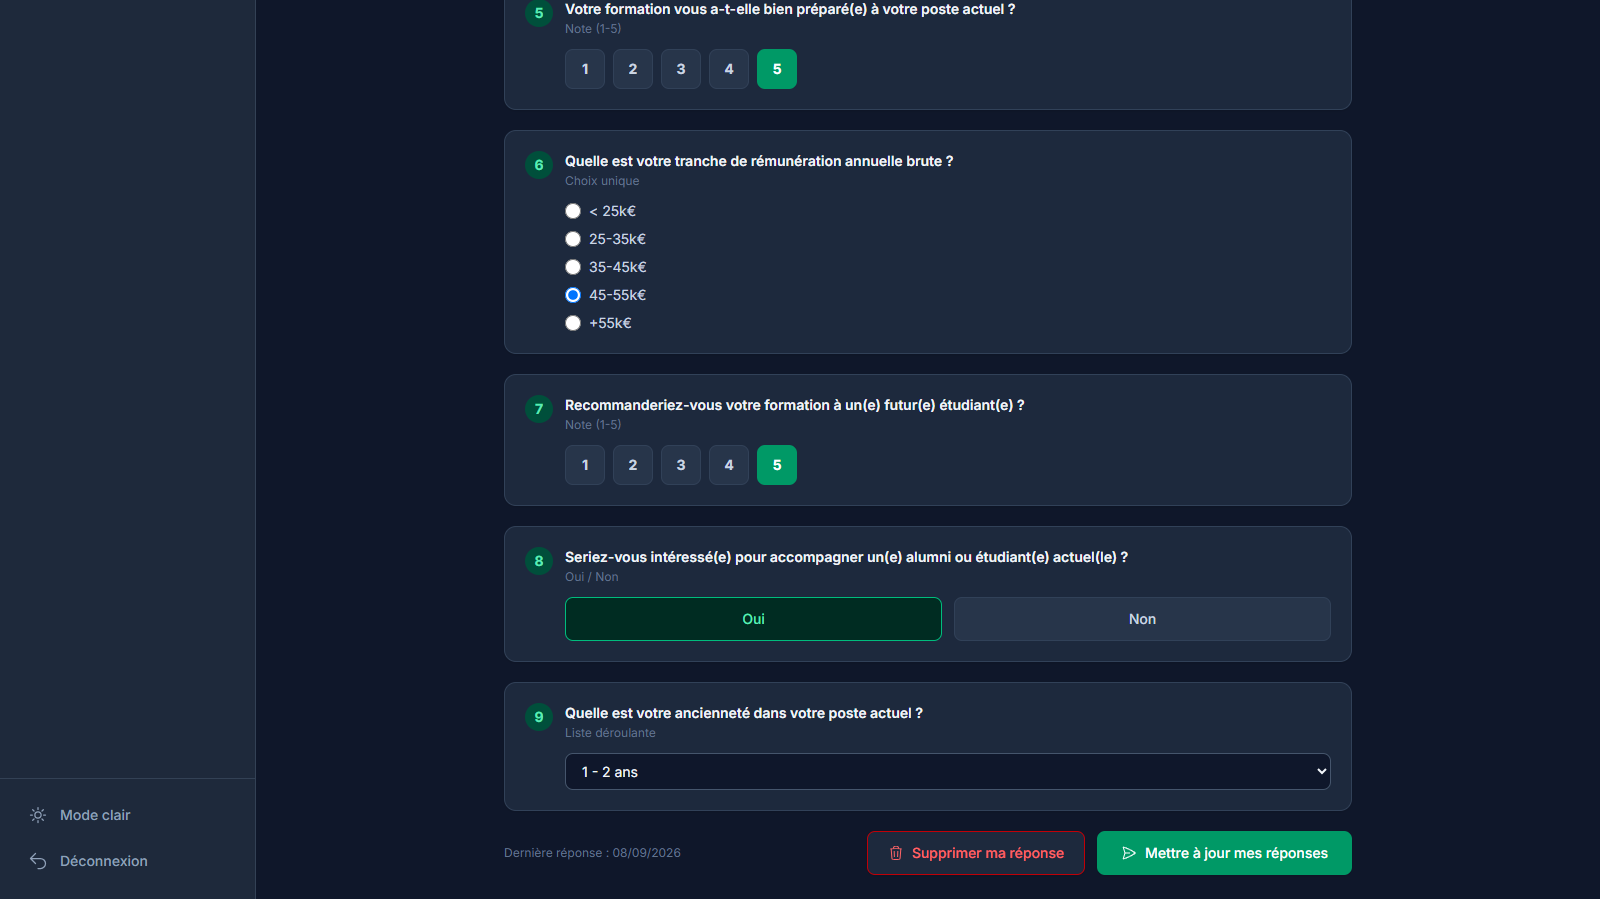
\includegraphics[width=\textwidth]{anC_questionnaire_dark_2.png}
    \caption{Mode sombre -- partie 2/2.}
  \end{minipage}
  \caption{Questionnaire annuel pré-rempli -- thème clair vs thème sombre, capture intégrale en deux parties.}
\end{figure}

\begin{figure}[htbp]
  \centering
  \begin{minipage}{0.48\textwidth}
    \centering
    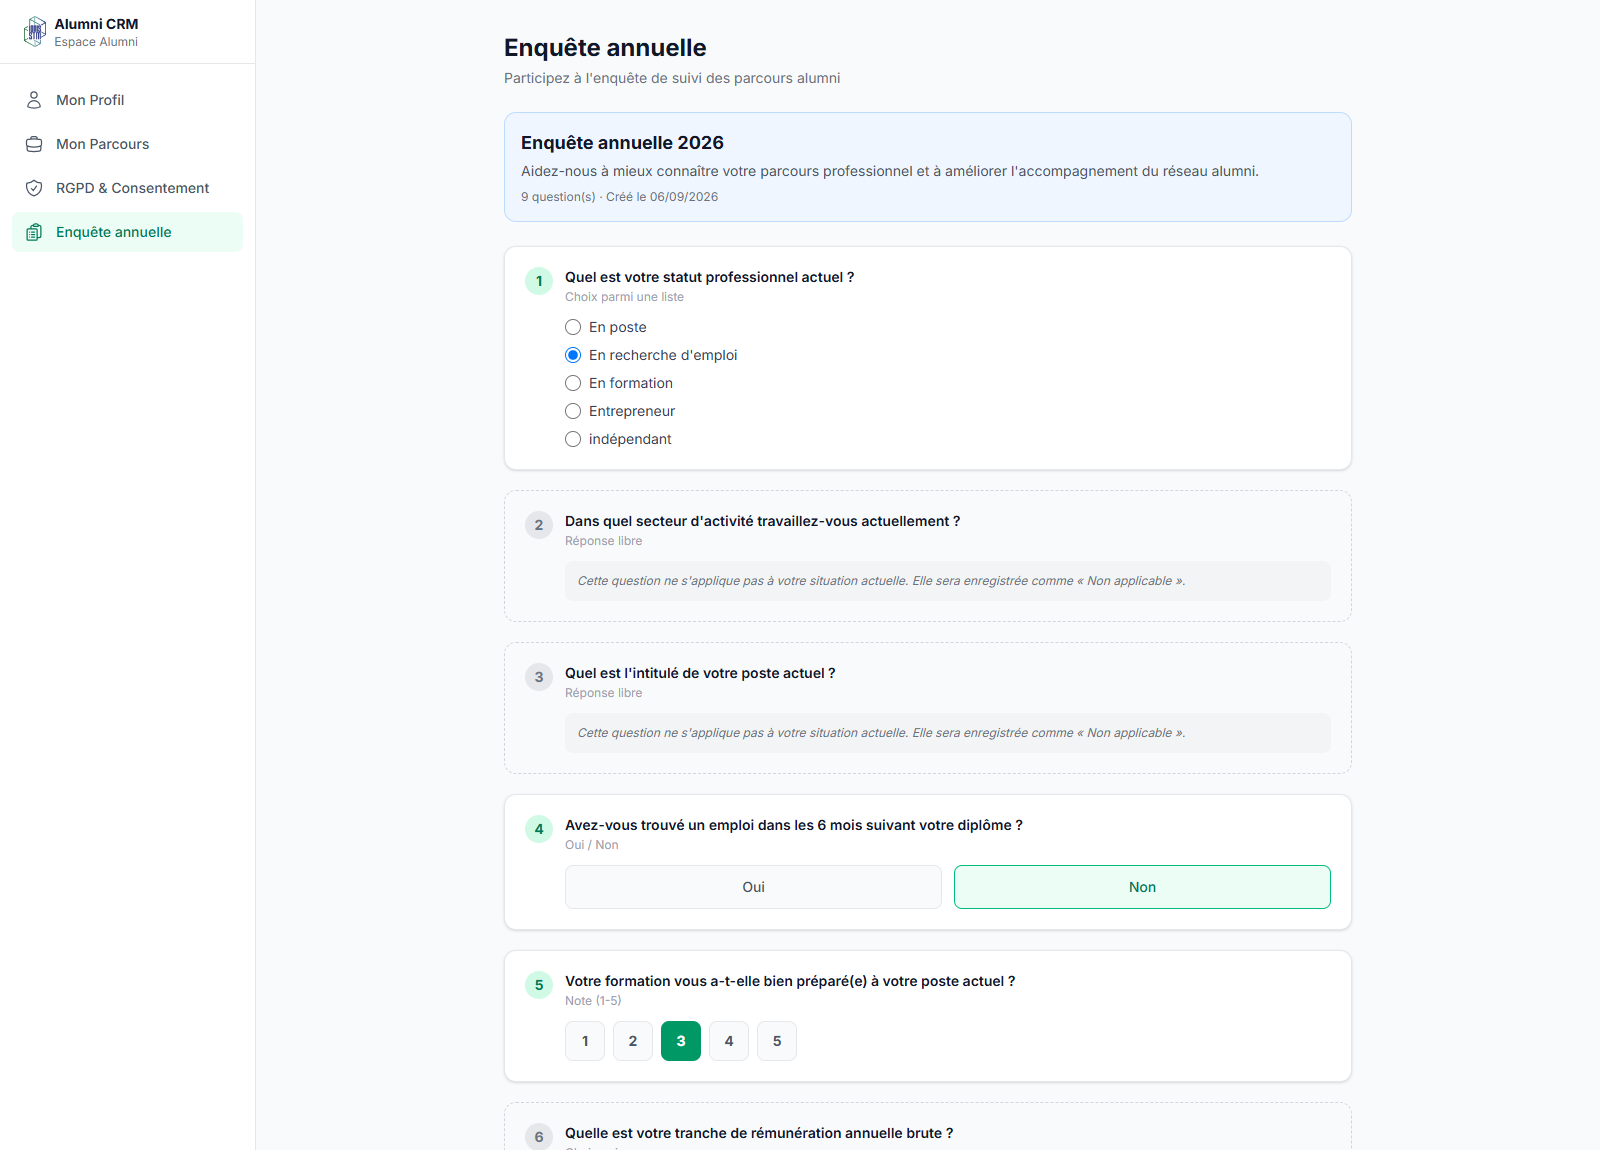
\includegraphics[width=\textwidth]{anC_questionnaire_recherche_light_1.png}
    \caption{Mode clair -- partie 1/2.}
  \end{minipage}\hfill
  \begin{minipage}{0.48\textwidth}
    \centering
    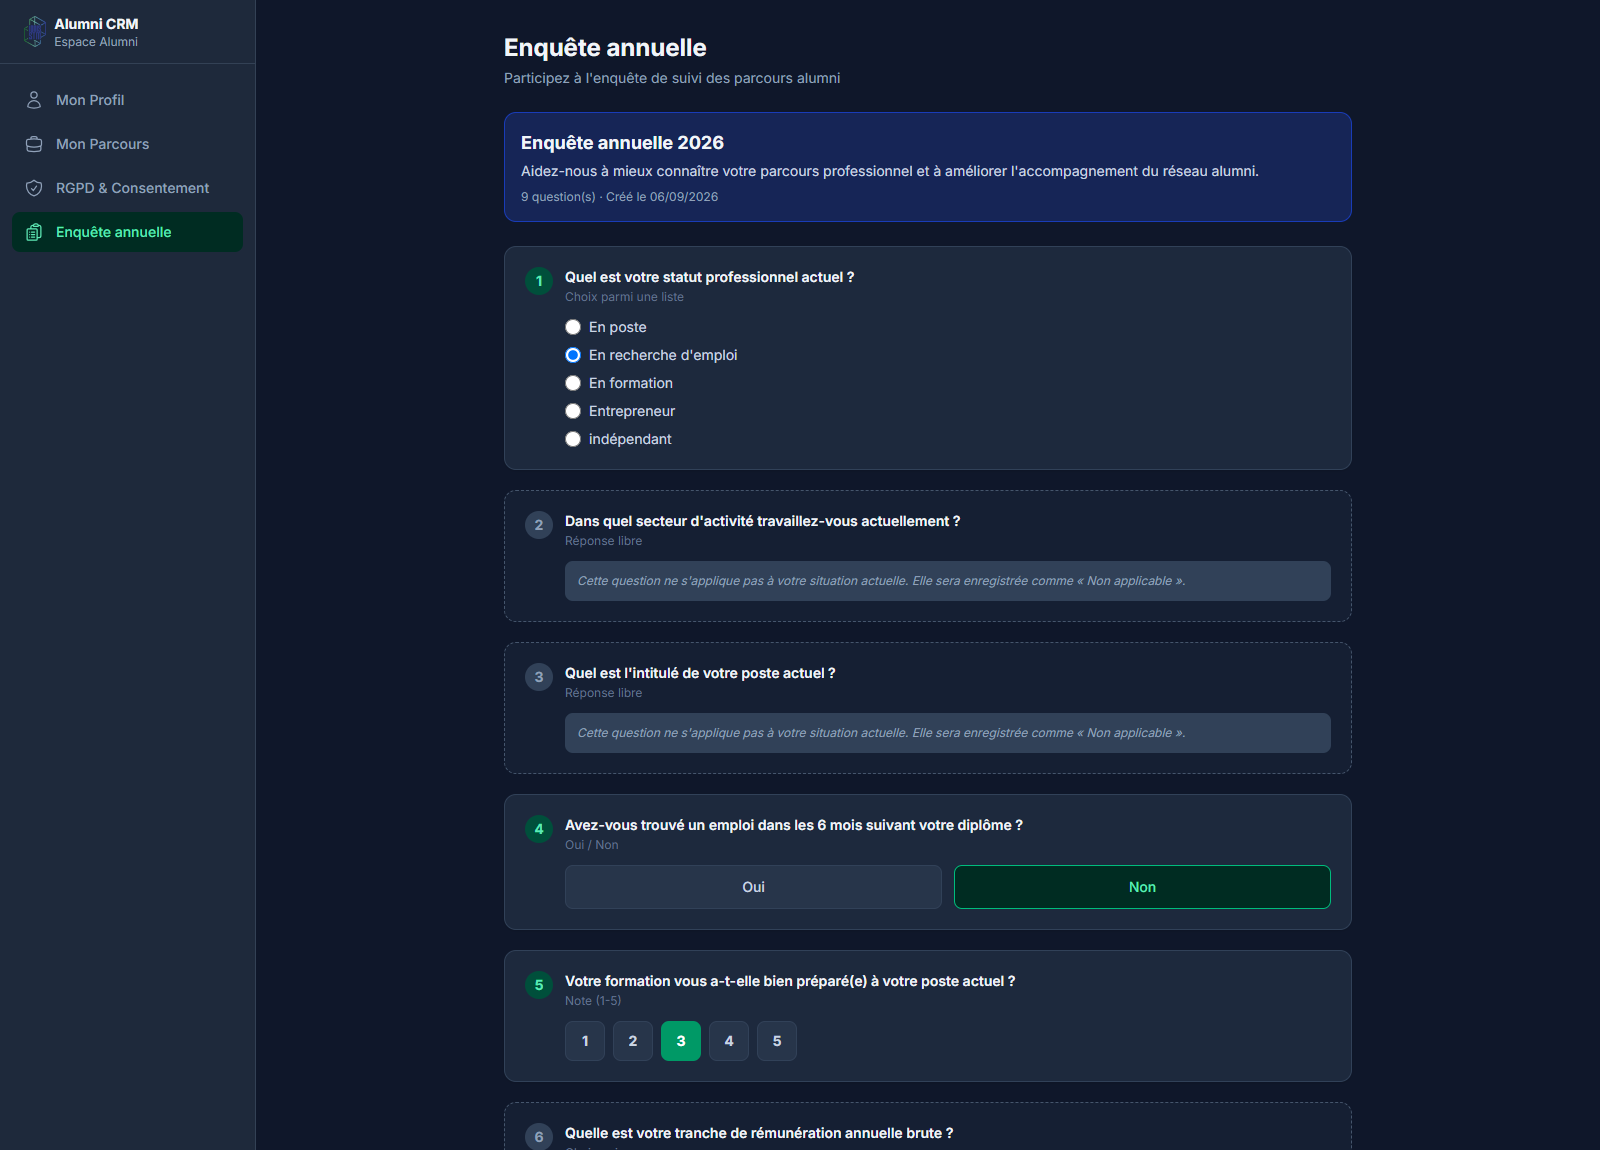
\includegraphics[width=\textwidth]{anC_questionnaire_recherche_dark_1.png}
    \caption{Mode sombre -- partie 1/2.}
  \end{minipage}

  \medskip

  \begin{minipage}{0.48\textwidth}
    \centering
    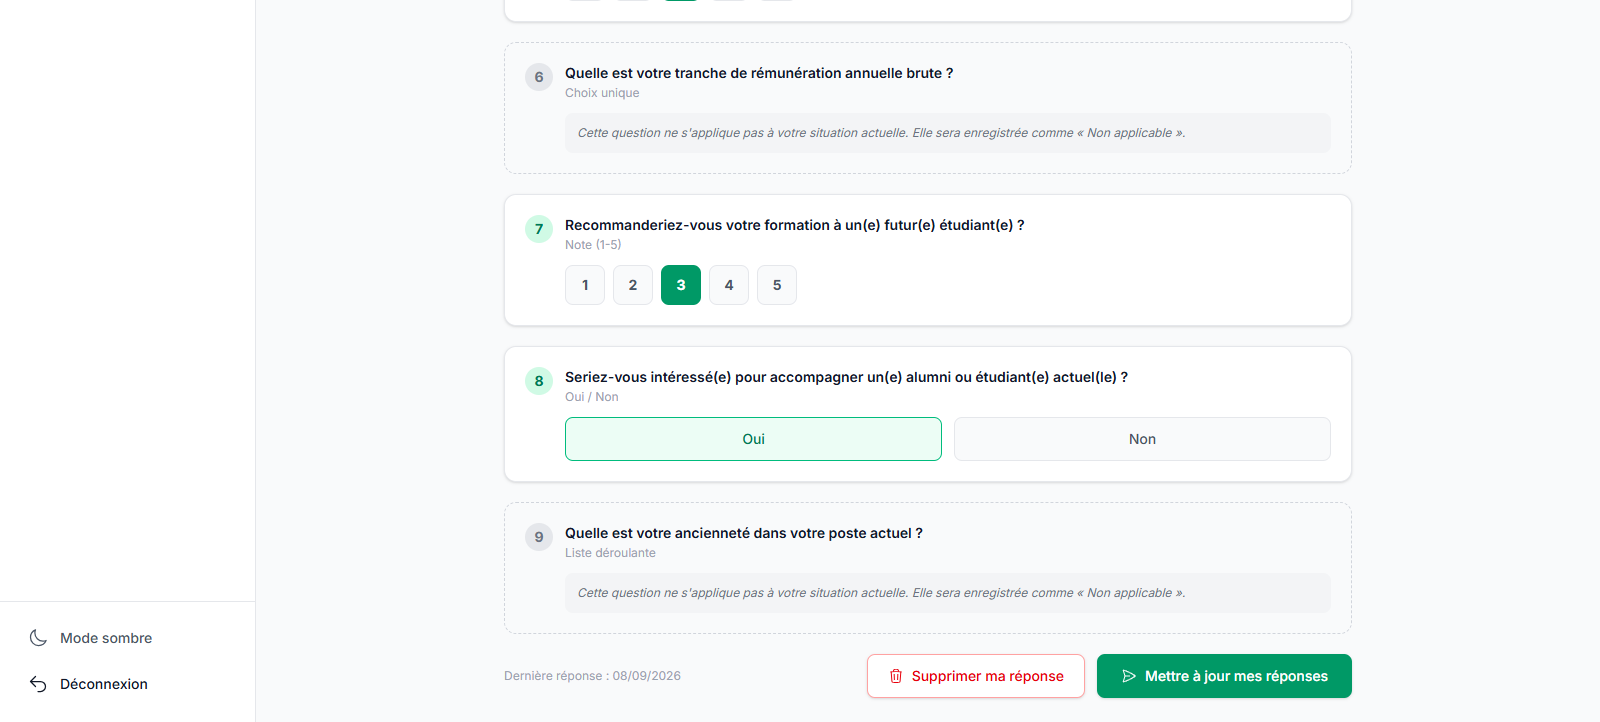
\includegraphics[width=\textwidth]{anC_questionnaire_recherche_light_2.png}
    \caption{Mode clair -- partie 2/2.}
  \end{minipage}\hfill
  \begin{minipage}{0.48\textwidth}
    \centering
    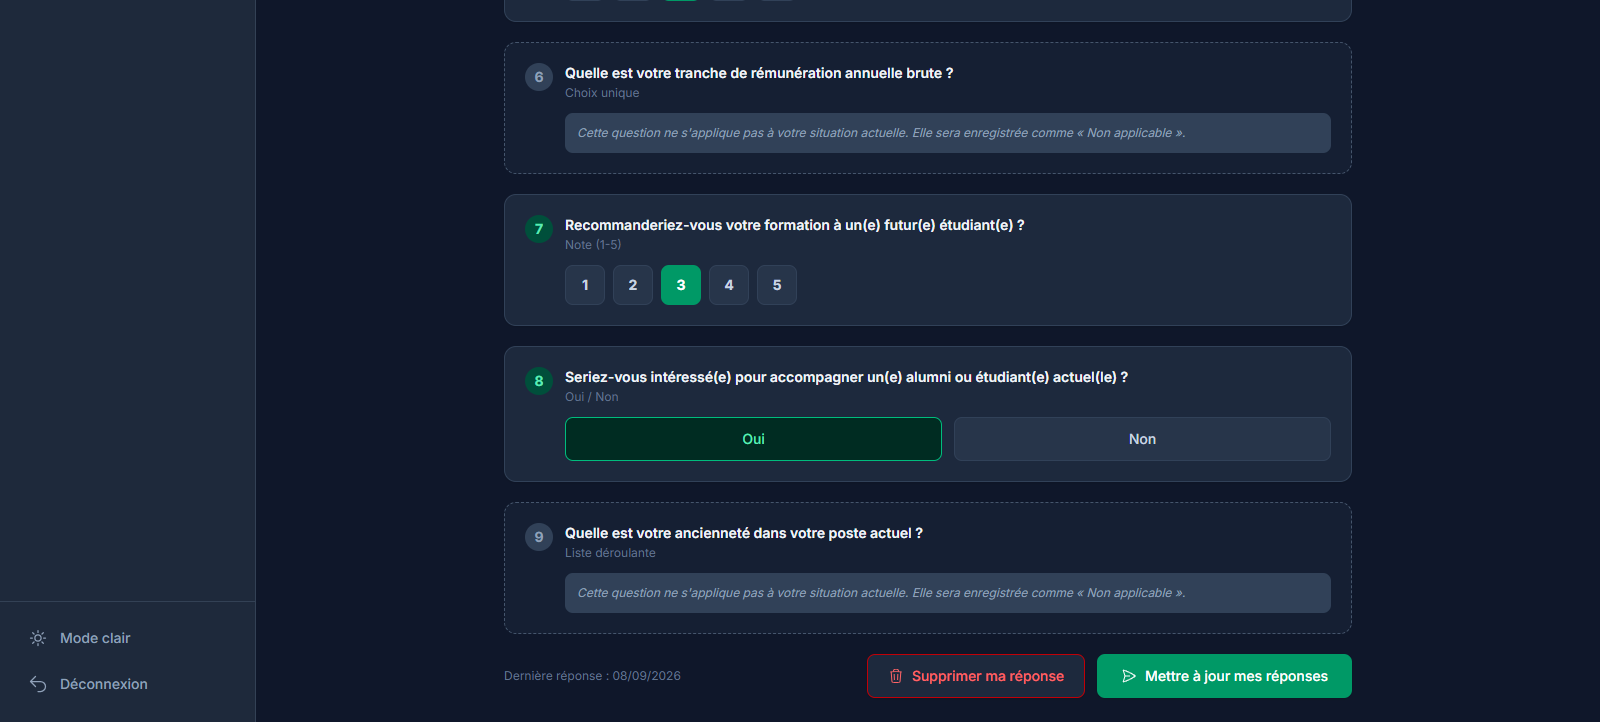
\includegraphics[width=\textwidth]{anC_questionnaire_recherche_dark_2.png}
    \caption{Mode sombre -- partie 2/2.}
  \end{minipage}
  \caption{Questionnaire annuel pour un alumni en recherche active -- questions conditionnées marquées \emph{Non applicable} -- thème clair vs thème sombre, capture intégrale en deux parties.}
\end{figure}

\begin{figure}[htbp]
  \centering
  \begin{minipage}{0.48\textwidth}
    \centering
    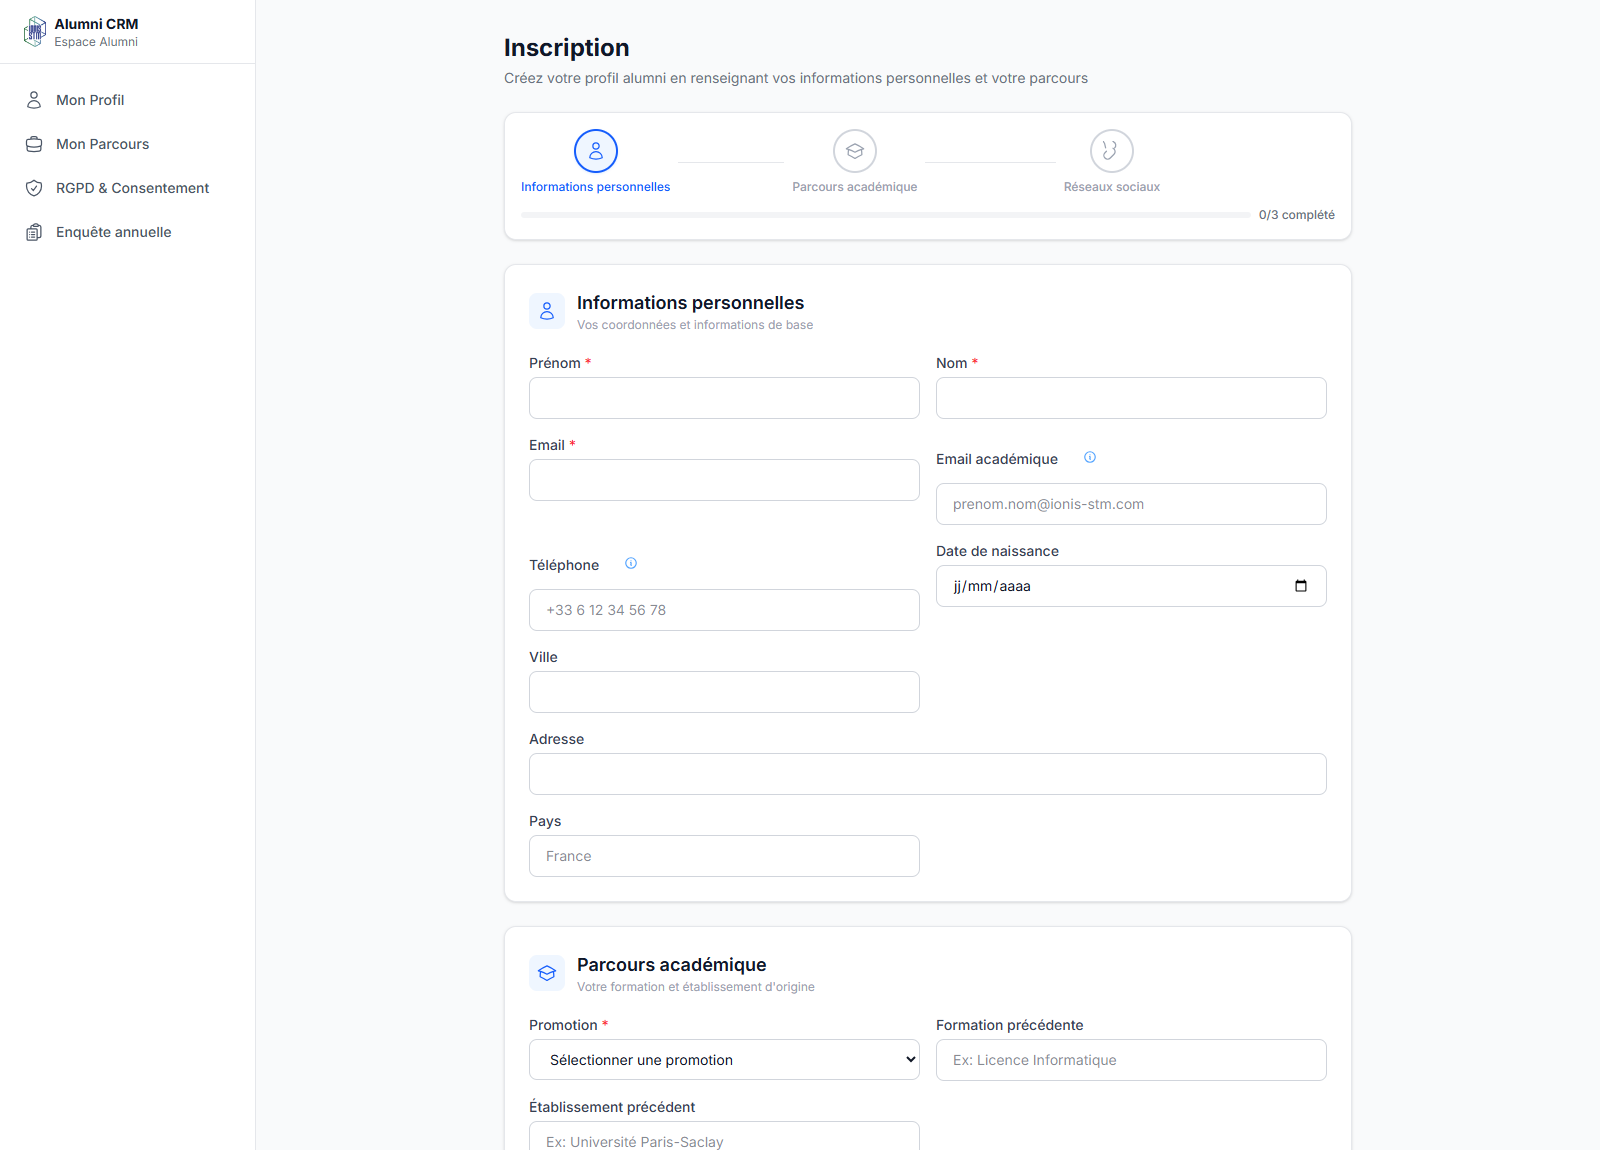
\includegraphics[width=\textwidth]{anC_inscription_light_1.png}
    \caption{Mode clair -- partie 1/2.}
  \end{minipage}\hfill
  \begin{minipage}{0.48\textwidth}
    \centering
    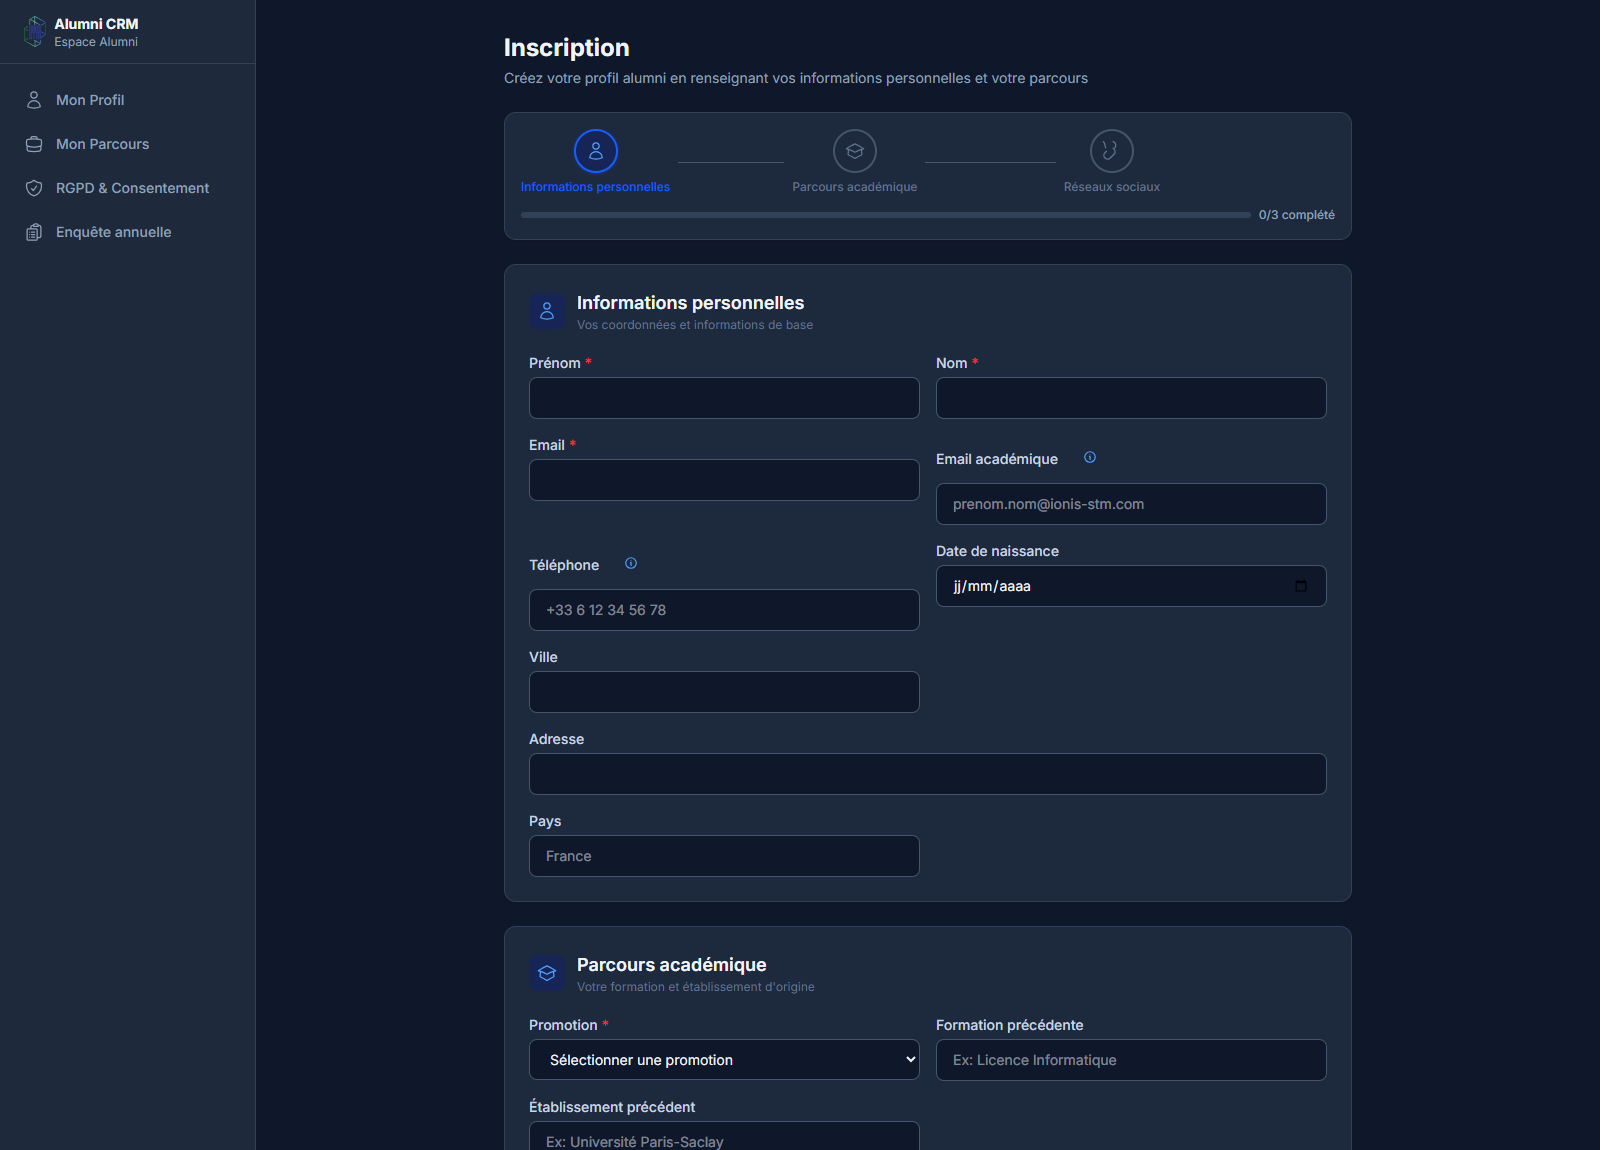
\includegraphics[width=\textwidth]{anC_inscription_dark_1.png}
    \caption{Mode sombre -- partie 1/2.}
  \end{minipage}

  \medskip

  \begin{minipage}{0.48\textwidth}
    \centering
    
\includegraphics[width=\textwidth]{anC_inscription_light_2.png}
    \caption{Mode clair -- partie 2/2.}
  \end{minipage}\hfill
  \begin{minipage}{0.48\textwidth}
    \centering
    
\includegraphics[width=\textwidth]{anC_inscription_dark_2.png}
    \caption{Mode sombre -- partie 2/2.}
  \end{minipage}
  \caption{Inscription multi-étapes (données personnelles, promotion, consentements RGPD) -- thème clair vs thème sombre, capture intégrale en deux parties.}
\end{figure}

\chapter{Cartographie des données (synthèse)}

\label{app:cartographie}
La cartographie complète est livrée séparément~: \texttt{Cartographie des Donnees - Alumni CRM.pdf}. Elle inventorie toutes les données traitées par le système, structurées par phase de vie.

\textbf{Phase d'inscription (données à l'entrée).} Identité et coordonnées (nom, prénom, email, téléphone, date de naissance, adresse, ville, pays, LinkedIn), statut et compétences (\texttt{availability\_status}, tags de compétences), historique académique (\texttt{parcours\_anterieur}, \texttt{previous\_school}), rattachement scolaire (\texttt{id\_promotion} $\rightarrow$ promotion, année de diplôme, filière), et données complémentaires (date d'inscription, email académique).

\textbf{Phase post-diplôme (données à la sortie).} Suivi des postes (entreprise, poste, type de contrat, dates de début/fin, poste actuel, description, salaire annuel \texttt{NUMERIC}, pays, ville, secteur), certifications (nom, émetteur, date d'obtention) et réponses aux questionnaires (réponses \hyperlink{abbr-JSON}{JSON~(20)}, années).

\textbf{Données de consentement \hyperlink{abbr-RGPD}{RGPD~(40)}.} La table \texttt{CONSENTEMENT\_RGPD} trace les 4 types de consentement (type, date, statut, canal), la table \texttt{DEMANDE\_RGPD} le workflow de traitement, et \texttt{AUDIT\_LOG} le journal horodaté des opérations sensibles.

\chapter{Charte de conformité RGPD (synthèse)}

\label{app:rgpd}
La charte complète est livrée séparément~: \texttt{Charte de Conformite RGPD - Alumni CRM.pdf}.

\textbf{Contexte juridique.} Le système est conforme au Règlement (\hyperlink{abbr-UE}{UE~(46)}) 2016/679 et à la loi Informatique et Libertés. Les données personnelles sont protégées par les mécanismes standard de \hyperlink{abbr-PostgreSQL}{PostgreSQL~(33)}~; aucun chiffrement applicatif spécifique n'est mis en œuvre à ce jour, et la notification de violation (article~33) reste manuelle.

\textbf{Les 4 types de consentement.}

\begin{table}[htbp]
\centering
\caption{Les 4 types de consentement RGPD : type backend, clé frontend et description.}
\label{tab:consentements}
\rowcolors{2}{gray!8}{white}
\begin{tabularx}{\textwidth}{@{} l *{2}{>{\raggedright\arraybackslash}X} @{}}
\toprule
\textbf{Type backend} & \textbf{Clé frontend} & \textbf{Description} \\
\midrule
\texttt{prise\_de\_contact} & \texttt{contact\_allowed} & L'école et les partenaires peuvent contacter l'alumni \\
\texttt{partage\_donnees} & \texttt{data\_sharing} & Données statistiques anonymisées partagées \\
\texttt{enquetes} & \texttt{survey\_participation} & Participation aux enquêtes alumni \\
\texttt{newsletter} & \texttt{newsletter} & Réception de la newsletter \\
\bottomrule
\end{tabularx}
\end{table}

\textbf{Consommation fonctionnelle des consentements.}
\begin{itemize}
  \item \texttt{newsletter}~: cible l'envoi via \texttt{/newsletter/envoyer}~;
  \item \texttt{enquetes}~: ouvre l'accès au questionnaire actif (refus $\rightarrow$ 403 et menu masqué)~;
  \item \texttt{prise\_de\_contact}~: le refus exclut des relances et déclenche l'anonymisation du profil via \texttt{cleanup.py} (seul consentement dont le refus anonymise)~;
  \item \texttt{partage\_donnees}~: alimente les indicateurs partenaires (\texttt{/admin/indicateurs/partenaires}).
\end{itemize}

\textbf{Droits \hyperlink{abbr-RGPD}{RGPD~(40)} implémentés.} Accès (export \hyperlink{abbr-JSON}{JSON~(20)}/Excel/\hyperlink{abbr-CSV}{CSV~(8)} auto-service), rectification (page profil), effacement (workflow demandes $\rightarrow$ anonymisation $\rightarrow$ purge différée de 6 mois), retrait du consentement (toggles). Toutes les opérations sont tracées dans \texttt{AUDIT\_LOG}.

\chapter{Stratégie de mise à jour des données (synthèse)}

\label{app:strategie}
La stratégie complète est livrée séparément~: \texttt{Strategie de Mise a Jour des Donnees - Alumni CRM.pdf}.

\textbf{Le défi de l'obsolescence.} Le principal défi d'un annuaire d'anciens est sa pérémption rapide (postes, entreprises, salaires). La gouvernance repose sur un processus proactif d'incitation à la mise à jour.

\textbf{Mise à jour manuelle par l'alumni.} Le profil (\texttt{AlumniProfile.jsx}) permet la modification de tous les champs personnels, le statut de disponibilité étant obligatoire et les compétences en tags dynamiques. Le parcours (\texttt{AlumniCareer.jsx}) gère l'ajout/suppression d'expériences et certifications, avec détection automatique du poste actuel et alerte visuelle en cas d'incohérence entre le statut \og{}en\_poste\fg{} et l'absence de poste actuel.

\textbf{Questionnaire annuel automatisé.} Côté admin, création/modification/suppression de questionnaires, 6 types de questions, tags \hyperlink{abbr-KPI}{KPI~(23)}, questions conditionnées et cycle de vie. Côté alumni, accès au questionnaire actif, pré-remplissage et questions conditionnées masquées.

\textbf{Pilotage par le service Relations Entreprises.} Création et administration des campagnes, tags \hyperlink{abbr-KPI}{KPI~(23)} alimentant automatiquement les indicateurs, relances automatiques (\texttt{\hyperlink{abbr-POST}{POST~(32)} /admin/questionnaires/notififier}). La newsletter constitue le principal canal de réactivation, avec un appel à l'action orienté vers la mise à jour du profil.

\chapter{Analyse des indicateurs d'insertion (synthèse)}

\label{app:indicateurs}
L'analyse complète est livrée séparément~: \texttt{Analyse des Indicateurs d'Insertion - Alumni CRM.pdf}.

\textbf{Principe.} Transformer les données brutes du \hyperlink{abbr-CRM}{CRM~(5)} en indicateurs de performance stratégiques pour les rapports d'insertion professionnelle requis par les organismes de certification (\hyperlink{abbr-CTI}{CTI~(9)}, \hyperlink{abbr-HCERES}{HCERES~(16)}) et les ministères.

\textbf{Principes généraux de calcul.}
\begin{itemize}
  \item \textbf{Comptes anonymisés exclus}~: toute ligne avec \texttt{date\_anonymisation IS NOT NULL} est exclue de tous les indicateurs (\hyperlink{abbr-RGPD}{RGPD~(40)}).
  \item \textbf{Source de vérité de l'emploi}~: la table \texttt{EXPERIENCE\_PRO} (et non le champ déclaratif \texttt{availability\_status}). Un alumni est \og{}en emploi\fg{} si une expérience est en cours.
  \item \textbf{Salaire}~: \texttt{salary\_annuel} (numérique) prioritaire, avec repli sur le champ texte historique.
  \item \textbf{Seuils d'affichage}~: secteur et type de contrat vides regroupés sous \og{}Non renseigné\fg{}~; au-delà de 6 catégories, regroupement sous \og{}Autres\fg{}.
\end{itemize}

\textbf{Les indicateurs de base et leurs endpoints.} Le tableau ci-dessous recense les indicateurs calculés indépendamment des questionnaires ; le total affiché dans le dashboard s'y ajoute d'un indicateur par question taguée active.

\begin{table}[htbp]
\centering
\caption{Synthèse des indicateurs d'insertion et leurs endpoints.}
\label{tab:indicateurs-endpoints}
\rowcolors{2}{gray!8}{white}
\begin{tabularx}{\textwidth}{@{} l >{\raggedright\arraybackslash}X @{}}
\toprule
\textbf{Indicateur} & \textbf{Calcul / endpoint} \\
\midrule
Total alumni actifs & \texttt{COUNT(*)} où \texttt{date\_anonymisation IS NULL} \\
Alumni actifs ($\geq$ 1 expérience) & \texttt{COUNT(DISTINCT id\_etudiant)} depuis \texttt{EXPERIENCE\_PRO} \\
Taux de complétion & (alumni avec $\geq$ 1 expérience / total) $\times$ 100 \\
Taux d'emploi à 6 mois & expérience active à la date de référence (fenêtre 6 mois)~; promo non mature $\rightarrow$ \texttt{null} \\
Taux d'emploi global & (étudiants en poste / total) $\times$ 100 par promotion \\
Répartition par secteur & \texttt{COUNT(DISTINCT id\_etudiant)} par secteur (poste actuel) \\
Alumni par promotion & effectif, \% en poste, taux de couverture, salaire moyen \\
Salaire moyen & \texttt{AVG} de \texttt{salary\_annuel} (ou repli)~; jauge avec échantillon $\geq$ 5 \\
Répartition par type de contrat & \texttt{COUNT(*)} des expériences en cours \\
\bottomrule
\end{tabularx}
\end{table}

\textbf{Endpoints \hyperlink{abbr-API}{API~(1)}.}
\begin{itemize}
  \item \texttt{\hyperlink{abbr-GET}{GET~(15)} /admin/indicateurs}
  \item \texttt{/admin/indicateurs/secteurs}
  \item \texttt{/admin/indicateurs/types-contrat}
  \item \texttt{/admin/indicateurs/kpi-tag}
  \item \texttt{/admin/indicateurs/kpi-tags}
  \item \texttt{/admin/indicateurs/kpi-tags-actifs}
  \item \texttt{/admin/indicateurs/partenaires}
\end{itemize}

\textbf{Cas limites.}
\begin{itemize}
  \item Promotion sans fenêtre de 6 mois écoulée $\rightarrow$ \texttt{null} + statut \og{}en\_attente\fg{}~;
  \item échantillon de salaire $<$ 5 $\rightarrow$ fourchette élargie et mention \og{}échantillon limité\fg{}~;
  \item tag \hyperlink{abbr-KPI}{KPI~(23)} sans réponse $\rightarrow$ état vide.
\end{itemize}

\chapter{Guide des processus d'animation du réseau (extrait)}

Le guide complet est livré séparément~: \texttt{Guide des Processus - Animation du Reseau Alumni.pdf}, également généré par script (\texttt{generate\_reports.py}). Il décrit \textbf{8 processus opérationnels} destinés au service Relations Entreprises et à l'équipe pédagogique~:

\begin{enumerate}
  \item \textbf{Inscription et collecte initiale}~: inscription multi-étapes, validation de l'email académique, 4 consentements \hyperlink{abbr-RGPD}{RGPD~(40)}~; import en masse via template Excel avec rapport d'erreur.
  \item \textbf{Suivi de l'insertion professionnelle}~: mise à jour par l'alumni (ajout/suppression d'expériences et certifications), référentiel de 37 secteurs standardisés.
  \item \textbf{Questionnaire annuel}~: création admin (6 types de questions, tags \hyperlink{abbr-KPI}{KPI~(23)}, conditions), réponse alumni pré-remplie, exploitation des \hyperlink{abbr-KPI}{KPI~(23)}.
  \item \textbf{Newsletter}~: ciblage par consentement, calendrier mensuel/bimestriel, contenu type avec CTA vers la mise à jour de profil.
  \item \textbf{Animation du réseau}~: annuaire filtrable, entretiens de suivi, événements trimestriels, identification des entreprises comptant le plus d'alumni.
  \item \textbf{Conformité \hyperlink{abbr-RGPD}{RGPD~(40)}}~: consentement traçable, workflow de demandes, export, audit.
  \item \textbf{Nettoyage et maintenance}~: détection d'orphelins, fusion de doublons, archivage, purge différée.
  \item \textbf{Pilotage}~: indicateurs de performance, suivi des campagnes.
\end{enumerate}

\chapter{Liste des endpoints API}

L'\hyperlink{abbr-API}{API~(1)} expose \textbf{84 endpoints} \hyperlink{abbr-REST}{REST~(39)} répartis sur \textbf{16 routeurs} (60 chemins). La liste exhaustive des méthodes et chemins est consultable directement dans la documentation \hyperlink{abbr-Swagger}{Swagger~(44)} générée automatiquement par FastAPI (endpoint \texttt{/docs}). Les principaux domaines sont~: Racine (1), Authentification (3), Promotions (5), Étudiants (7), Entreprises (5), Expériences (6), Certifications (8), \hyperlink{abbr-RGPD}{RGPD~(40)} alumni (7), \hyperlink{abbr-RGPD}{RGPD~(40)} admin (11), Annuaire/Indicateurs (8), Nettoyage (6), Import/Export (3), Questionnaires alumni (4), Questionnaires admin (9), Newsletter (1).

\textbf{Documentation \hyperlink{abbr-Swagger}{Swagger~(44)} (FastAPI).} La figure suivante montre la page \texttt{/docs} générée automatiquement, avec la liste des routeurs et la console d'essai intégrée.

\begin{figure}[htbp]
  \centering
  \begin{minipage}{0.48\textwidth}
    \centering
    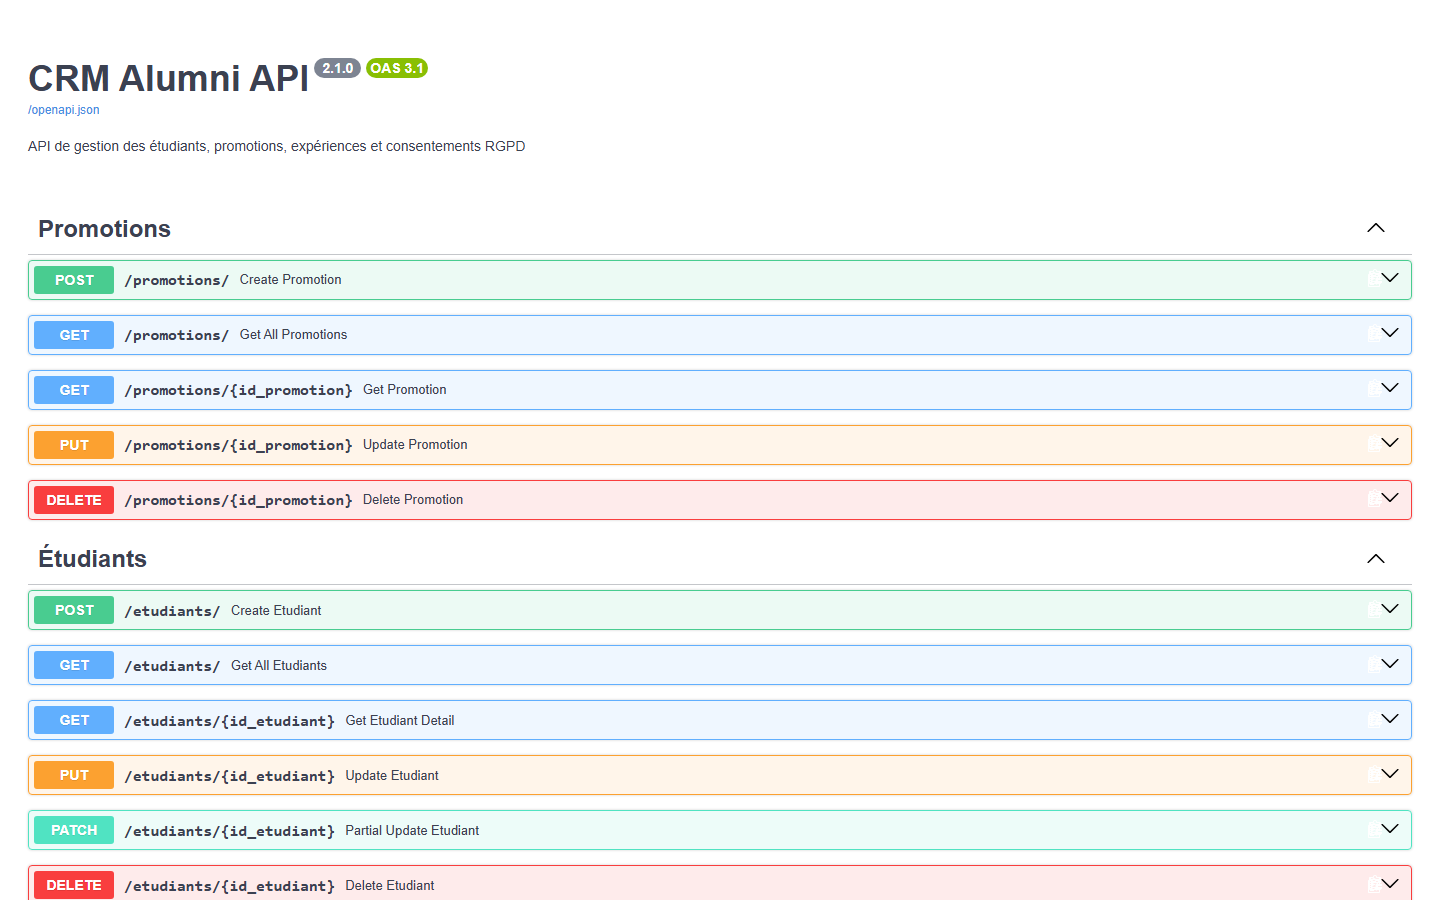
\includegraphics[width=\textwidth]{swagger_light.png}
    \caption{Mode clair.}
  \end{minipage}\hfill
  \begin{minipage}{0.48\textwidth}
    \centering
    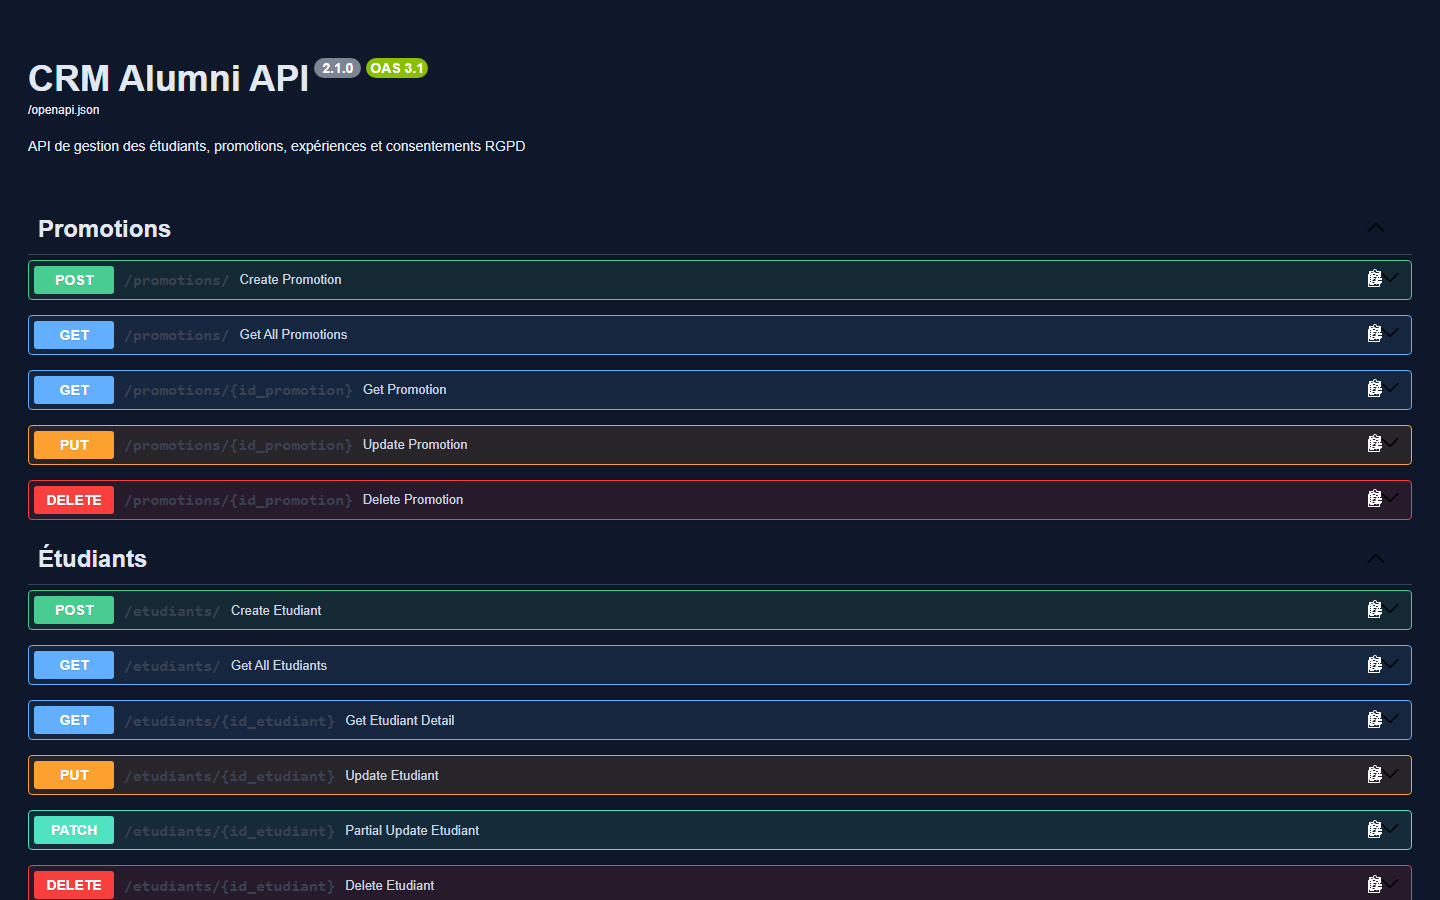
\includegraphics[width=\textwidth]{swagger_dark.png}
    \caption{Mode sombre.}
  \end{minipage}
  \caption{Documentation Swagger UI de l'API FastAPI (\texttt{/docs})}
  \label{fig:swagger}
\end{figure}

\vspace{0.5em}
\noindent\textbf{Exemples d'appels.} Quelques appels significatifs, avec le corps de requête envoyé et la réponse \hyperlink{abbr-JSON}{JSON~(20)} réellement retournée par l'\hyperlink{abbr-API}{API~(1)}. \texttt{<token>} désigne le jeton \hyperlink{abbr-JWT}{JWT~(22)} obtenu aux étapes 1 (admin) ou 3 (alumni), transmis dans l'en-tête \texttt{Authorization: Bearer <token>}.

% ── 1. Authentification admin ────────────────────────────────────
\subsubsection*{1. Authentification admin — \texttt{POST /auth/admin/login}}
\emph{Connexion de l'administrateur par code d'accès. Réponse~: jeton \hyperlink{abbr-JWT}{JWT~(22)} + rôle. Ce token protège toutes les routes \texttt{/admin/*}.}

\begin{lstlisting}[language=bash, caption={Authentification administrateur}, label={lst:curl-login}]
curl -X POST http://localhost:8000/auth/admin/login \
  -H "Content-Type: application/json" \
  -d '{"code": "s3cr3t"}'
\end{lstlisting}
\begin{lstlisting}[language=json, caption={Réponse — token JWT et rôle}, label={resp:curl-login}]
{
  "token": "eyJhbGciOiJIUzI1NiIsInR5cCI6IkpXVCJ9...",
  "role": "admin"
}
\end{lstlisting}

% ── 2. Demande d'un code OTP (28) ─────────────────────────────────────
\subsubsection*{2. Demande d'un code OTP — \texttt{POST /auth/otp/request}}
\emph{Déclenche l'envoi par email d'un code à 6 chiffres (10 min de validité). La réponse est volontairement identique que le compte existe ou non (anti-énumération d'adresses).}

\begin{lstlisting}[language=bash, caption={Envoi du code OTP par email}, label={lst:curl-otp}]
curl -X POST http://localhost:8000/auth/otp/request \
  -H "Content-Type: application/json" \
  -d '{"email": "jean.dupont@example.com"}'
\end{lstlisting}
\begin{lstlisting}[language=json, caption={Réponse — confirmation d'envoi}, label={resp:curl-otp}]
{
  "message": "Si ce compte existe, un code a ete envoye."
}
\end{lstlisting}

% ── 3. Vérification du code OTP (28) ──────────────────────────────────
\subsubsection*{3. Vérification du code OTP — \texttt{POST /auth/otp/verify}}
\emph{Échange du code reçu contre un jeton de session alumni (\hyperlink{abbr-JWT}{JWT~(22)}, rôle \texttt{alumni}, validité 24 h), accompagné des informations minimales du compte.}

\begin{lstlisting}[language=bash, caption={Vérification OTP}, label={lst:curl-otp-verify}]
curl -X POST http://localhost:8000/auth/otp/verify \
  -H "Content-Type: application/json" \
  -d '{"email": "jean.dupont@example.com", "code": "483920"}'
\end{lstlisting}
\begin{lstlisting}[language=json, caption={Réponse — token de session alumni}, label={resp:curl-otp-verify}]
{
  "token": "eyJhbGciOiJIUzI1NiIsInR5cCI6IkpXVCJ9...",
  "alumni": {
    "id_etudiant": 1,
    "nom": "Dupont",
    "prenom": "Jean",
    "email": "jean.dupont@example.com"
  },
  "role": "alumni"
}
\end{lstlisting}

% ── 4. Indicateurs du tableau de bord ────────────────────────────
\subsubsection*{4. Indicateurs du tableau de bord — \texttt{GET /admin/indicateurs} \emph{(route admin)}}
\emph{Indicateurs globaux~: taux d'emploi, salaires, couverture. Les champs \texttt{hypothese} et \texttt{source\_de\_verite} documentent les règles de calcul~; la réponse complète est tronquée (\texttt{...}) pour la lisibilité.}

\begin{lstlisting}[language=bash, caption={Requête indicateurs}, label={lst:curl-indicateurs}]
curl -X GET http://localhost:8000/admin/indicateurs \
  -H "Authorization: Bearer <token>"
\end{lstlisting}
\begin{lstlisting}[language=json, caption={Réponse — taux d'emploi et salaires par promotion}, label={resp:curl-indicateurs}]
{
  "hypothese": "diplomation juin, delai approxime : date de reference = annee_diplome-12-01 (+6 mois)...",
  "source_de_verite": "EXPERIENCE_PRO : experience non terminee... ; availability_status est declaratif...",
  "indicateurs_par_promotion": [
    {
      "nom_promotion": "Promotion 2023",
      "annee_diplome": 2023,
      "total_etudiants": 4,
      "etudiants_en_poste": 2,
      "etudiants_avec_experience": 3,
      "salaire_moyen": 3550.0,
      "taux_emploi_pourcentage": 50.0,
      "taux_couverture": 75.0
    }
  ],
  "taux_emploi_6mois_par_promotion": [
    {
      "nom_promotion": "Promotion 2023",
      "annee_diplome": 2023,
      "date_reference": "2023-12-01",
      "statut_maturite": "mature",
      "total_diplomes": 4,
      "emplois_6_mois": 3,
      "taux_emploi_6mois_pourcentage": 75.0,
      "taux_couverture": 75.0
    }
  ],
  "taux_emploi_6mois": 73.33,
  "total_diplomes_matures": 15,
  "emplois_6_mois_matures": 11,
  "alumni_actifs": 22,
  "taux_reponse": 91.67,
  "total_alumni": 24,
  "salaire_moyen": 46909.09,
  "salaires_renseignes": 11,
  "salaire_min": 32000.0,
  "salaire_max": 70000.0
}
\end{lstlisting}

% ── 5. Répartition par secteur ────────────────────────────────────
\subsubsection*{5. Répartition par secteur — \texttt{GET /admin/indicateurs/secteurs} \emph{(route admin)}}
\emph{Nombre d'alumni par secteur d'activité (secteur de l'expérience en cours). Un secteur absent est agrégé sous \texttt{"secteur": null} (affiché « Non renseigné » côté frontend).}

\begin{lstlisting}[language=bash, caption={Requête secteurs}, label={lst:curl-secteurs}]
curl -X GET http://localhost:8000/admin/indicateurs/secteurs \
  -H "Authorization: Bearer <token>"
\end{lstlisting}
\begin{lstlisting}[language=json, caption={Réponse — distribution par secteur d'activité}, label={resp:curl-secteurs}]
{
  "secteurs": [
    {"secteur": "Technologie", "count": 3},
    {"secteur": "Conseil", "count": 2},
    {"secteur": "Marketing", "count": 2},
    {"secteur": null, "count": 1}
  ],
  "total_alumni": 24
}
\end{lstlisting}

% ── 6. Tags KPI (23) des questionnaires actifs ────────────────────────
\subsubsection*{6. Tags KPI des questionnaires actifs — \texttt{GET /admin/indicateurs/kpi-tags} \emph{(route admin)}}
\emph{Indicateurs dérivés calculés automatiquement à partir des réponses des questionnaires actifs. Un tag sans réponse est toujours renvoyé (valeurs \texttt{null}).}

\begin{lstlisting}[language=bash, caption={Requête KPI tags}, label={lst:curl-kpi}]
curl -X GET http://localhost:8000/admin/indicateurs/kpi-tags \
  -H "Authorization: Bearer <token>"
\end{lstlisting}
\begin{lstlisting}[language=json, caption={Réponse — indicateurs dérivés du questionnaire}, label={resp:curl-kpi}]
[
  {
    "tag": "adequation_formation",
    "question_texte": "Votre formation vous a-t-elle prepare au monde professionnel ?",
    "question_type": "boolean",
    "total_repondants": 12,
    "valeur": 75.0,
    "unite": "%",
    "libelle_valeur": "Oui",
    "distribution": [
      {"label": "Oui", "nb": 9, "pourcentage": 75.0},
      {"label": "Non", "nb": 3, "pourcentage": 25.0}
    ],
    "detail": null,
    "reponses_recentes": [
      {"reponse": "oui", "date": "2026-06-01"},
      {"reponse": "non", "date": "2026-05-28"}
    ]
  }
]
\end{lstlisting}

% ── 7. Questionnaire actif ───────────────────────────────────────
\subsubsection*{7. Questionnaire actif — \texttt{GET /questionnaires/actif?id\_etudiant=1} \emph{(route alumni)}}
\emph{Questionnaire en cours de collecte avec ses questions dans l'ordre (\texttt{ordre}), le type (\texttt{boolean}, \texttt{choice}, \texttt{single\_choice}, \texttt{dropdown}, \texttt{rating}, \texttt{text}), les options (\texttt{options}) et le tag \hyperlink{abbr-KPI}{KPI~(23)} éventuel (\texttt{tag}).}

\begin{lstlisting}[language=bash, caption={Récupération du questionnaire courant}, label={lst:curl-questionnaire}]
curl -X GET "http://localhost:8000/questionnaires/actif?id_etudiant=1" \
  -H "Authorization: Bearer <token>"
\end{lstlisting}
\begin{lstlisting}[language=json, caption={Réponse — structure du questionnaire et questions}, label={resp:curl-questionnaire}]
{
  "id_questionnaire": 3,
  "titre": "Enquete Alumni 2026",
  "description": "Situation professionnelle un an apres l'obtention du diplome.",
  "date_creation": "2026-06-01",
  "actif": true,
  "questions": [
    {
      "id_question": 11,
      "id_questionnaire": 3,
      "texte": "Votre formation vous a-t-elle prepare au monde professionnel ?",
      "type": "boolean",
      "options": [],
      "ordre": 1,
      "tag": "adequation_formation",
      "conditionnee_statut_emploi": false
    },
    {
      "id_question": 12,
      "id_questionnaire": 3,
      "texte": "Dans quel secteur exercez-vous ?",
      "type": "dropdown",
      "options": ["Technologie", "Finance", "Sante", "Education", "Autre"],
      "ordre": 2,
      "tag": "secteur_emploi",
      "conditionnee_statut_emploi": true
    }
  ]
}
\end{lstlisting}

% ── 8. Consentements alumni ──────────────────────────────────────
\subsubsection*{8. Consentements RGPD d'un alumni — \texttt{GET /consentements/etudiant/\{id\}} \emph{(alumni ou admin)}}
\emph{Historique des choix, du plus récent au plus ancien. Chaque ligne est horodatée et porte le canal de collecte (\texttt{web})~; pour lire l'état courant il faut conserver la ligne la plus récente de chaque \texttt{type\_consentement}.}

\begin{lstlisting}[language=bash, caption={Lecture des consentements RGPD d'un alumni}, label={lst:curl-consent}]
curl -X GET http://localhost:8000/consentements/etudiant/1 \
  -H "Authorization: Bearer <token>"
\end{lstlisting}
\begin{lstlisting}[language=json, caption={Réponse — historique des consentements}, label={resp:curl-consent}]
[
  {
    "id_consentement": 42,
    "date_consentement": "2026-06-15",
    "type_consentement": "newsletter",
    "statut": "actif",
    "canal": "web",
    "id_etudiant": 1
  },
  {
    "id_consentement": 38,
    "date_consentement": "2026-06-10",
    "type_consentement": "prise_de_contact",
    "statut": "actif",
    "canal": "web",
    "id_etudiant": 1
  },
  {
    "id_consentement": 37,
    "date_consentement": "2026-06-10",
    "type_consentement": "enquetes",
    "statut": "actif",
    "canal": "web",
    "id_etudiant": 1
  },
  {
    "id_consentement": 36,
    "date_consentement": "2026-06-10",
    "type_consentement": "partage_donnees",
    "statut": "actif",
    "canal": "web",
    "id_etudiant": 1
  }
]
\end{lstlisting}

\chapter{Différentiel de migration et audit de conformité}

Le drift de migration (clé étrangère \texttt{ON \hyperlink{abbr-DELETE}{DELETE~(10)} \hyperlink{abbr-CASCADE}{CASCADE~(2)}} sur \texttt{reponse\_questionnaire.id\_etudiant} sans contrepartie dans le fichier de migration d'origine) a été corrigé par une migration corrective \textbf{idempotente} (011), et le rejeu complet des migrations sur une base vide (16 à la date de l'audit, 17 avec la migration corrective 016) ne relève aucune différence structurelle.

\textbf{Principe retenu.} Une migration déjà appliquée ne se modifie jamais~; on corrige par une nouvelle migration. C'est ainsi qu'a été traité le drift de la migration 003 par la migration corrective 011, qui interroge \texttt{pg\_constraint} avant d'agir.

\textbf{Points secondaires — état au 10/09/2026.} Les points P2 relevés ont été résolus~: statut des consentements contraint (\texttt{Literal} côté \hyperlink{abbr-API}{API~(1)} et \hyperlink{abbr-CHECK}{CHECK~(3)} en base, migration 016), date d'obtention des certifications validée (pas de date future), réponses de questionnaire contrôlées contre le type de la question, mise à jour atomique d'une expérience (\hyperlink{abbr-PUT}{PUT~(34)} /experiences/\{id\_experience\}), ordre 0 respecté, et réponses réelles du \texttt{actif} et du \texttt{nb\_etudiants}. Deux points de maintenance restent en P3~: la purge des tables \texttt{otp\_codes} et \texttt{AUDIT\_LOG} et l'échec silencieux de \texttt{\_write\_audit\_log}. Le détail est consigné dans \texttt{AUDIT\_COHERENCE.md} (synthèse + détail table-par-champ, PDF~: \texttt{AUDIT\_COHERENCE.pdf}).

\end{document}
